\documentclass[a4paper]{article}

\usepackage{fontspec}
%για επιλογή γραμματοσειρών
\usepackage{polyglossia}
%για συλλαβισμό λέξεων
\usepackage{geometry}
%για μορφή σελίδας a4
\usepackage{longtable}
%για προχωρημένους πίνακες
\usepackage{tabu}
%για προχωρημένους πίνακες
\usepackage[colorlinks=true,
            linkcolor=blue,
            urlcolor=blue,
            citecolor=gray]{hyperref}
%για όμορφα links
\usepackage{comment}
%για κομμάτια σχολίων

\setdefaultlanguage{greek}
\setotherlanguage{english}

\setmainfont{DejaVu Sans}

\title{Tutorial - Οδηγός Εκμάθησης KiCad}
\author{Μιχάλης Μισιρλής}
\date{Νοέμβριος 2015, έκδοση 1.2}

\begin{document}

\maketitle

\pagebreak
\tableofcontents
\pagebreak

\newpage
\section{Εισαγωγή}
Αυτός ο οδηγός εκμάθησης έχει ως στόχο την εξοικείωση του Έλληνα χρήστη του \textenglish{KiCad} μέσα από την ανάπτυξη ενός απλού αλλά πλήρους κυκλώματος (ηλεκτρονική συσκευή) ξεκινώντας από την βασική ιδέα και το σκοπό της συσκευής και καταλήγοντας στην παραγωγή αρχείων κατασκευής ώστε να μπορεί να παραχθεί η συσκευή από οποιοδήποτε εργοστάσιο ή εταιρεία παραγωγής πλακετών.

\subsection{Προαπαιτούμενα}
\label{sec:prereq}
Αυτός ο οδηγός έχει βασιστεί και απαιτεί το πρόγραμμα \textenglish{KiCad} έκδοση 4.0.0 με το Ελληνικό περιβάλλον λειτουργίας (GUI).

Ο οδηγός θεωρεί ότι ο χρήστης είναι εξοικειωμένος με τις βασικές έννοιες ηλεκτρονικού σχεδιασμού και μπορεί να σχεδιάσει πλήρως ένα κύκλωμα στο χαρτί ή σε κάποιο άλλο πρόγραμμα. Αυτός ο οδηγός δεν έχει ως στόχο τη διδασκαλία ηλεκτρονικού σχεδιασμού, αλλά τη διδασκαλία του πως γίνεται ο ηλεκτρονικός σχεδιασμός με το \textenglish{KiCad}. Επίσης ο οδηγός θεωρεί ότι ο χρήστης είναι εξοικειωμένος τις βασικές έννοιες χρήσης ηλεκτρονικών υπολογιστών, όπως επιλογή μενού, έξοδος από ένα παράθυρο, επιλογή πολλαπλών στοιχείων κα.

% έκδοση kicad
% έκδοση ελλ μετάφρασης

Το tutorial αυτό πρέπει να συνοδεύεται από αρχείο zip (kicad\_tut018) τo οποίο περιέχει όλα τα σχετικά αρχεία του \textenglish{KiCad}. 

Η σελίδα του οδηγού στο διαδίκτυο μπορεί να βρεθεί στον παρακάτω σύνδεσμο:\\
\href{https://github.com/ellak-monades-aristeias/KiCad\_EDA\_Greece}{https://github.com/ellak-monades-aristeias/KiCad\_EDA\_Greece}


\subsection{Λεξικό όρων}
\begin{longtabu}{ l l }
    \textbf{Ελληνικός όρος}	&	\textbf{Αγγλικός όρος}	\\
    3Δ προβολή	&	3d viewer	\\
    αγκύρωση	&	anchor	\\
    ακροδέκτης	&	pin	\\
    ακτίνα	&	spoke	\\
    αλφαριθμητικό	&	string	\\
    ανάλυση	&	parse	\\
    αναφορά, ονομασία αναφοράς	&	reference	\\
    αντεστραμμένο	&	inverted	\\
    αντικολλητική μάσκα	&	solder resist mask	\\
    αντίσταση συγκόλλησης	&	solder resist	\\
    απόδοση	&	render	\\
    απόκλιση	&	skew	\\
    αποτύπωμα	&	footprint	\\
    γομα	&	eraser	\\
    γραμμή γραφικών	&	graphic line	\\
    διάκενο	&	clearance	\\
    διαμπερές	&	through (hole)	\\
    διάτρηση	&	drill	\\
    δίαυλος	&	bus	\\
    δίκτυα μίας έδρας	&	single pad nets	\\
    δρομολόγηση	&	route	\\
    δρόμος	&	pcb trace / track	\\
    έδρα	&	antipad	\\
    έδρα	&	pad	\\
    ΕΗΚ, Έλεγχος Ηλεκτρικών Κανόνων	&	ERC, Electronics Rules Check	\\
    ΕΚΣ, Έλεγχος Κανόνων Σχεδίασης	&	DRC, Design Rules Check	\\
    εξάρτημα	&	component	\\
    έξοδος	&	output	\\
    επάνω πλευρά	&	top side	\\
    επεξεργαστής σχεδίασης σελίδας	&	page layout editor	\\
    επιλογή	&	option / choice / selection	\\
    επίπεδο	&	layer	\\
    επίπεδο eco	&	eco layer	\\
    επίπεδο σχεδίων	&	drawings layer	\\
    επίπεδο επικόλλησης	&	adhesive layers	\\
    επισήμανση	&	flag	\\
    ζώνη	&	zone	\\
    θαμμένο via	&	buried via	\\
    θύρα	&	port	\\
    θύρα ισχύος	&	power port	\\
    κατοπτρισμός, καθρέφτισμα	&	mirror	\\
    κάτω πλευρά	&	bottom side	\\
    κενό	&	gap	\\
    κοίλες γωνίες	&	fillet	\\
    κώδικας g	&	g code	\\
    λειτουργία γεμίσματος	&	filled mode	\\
    λειτουργία περιγράμματος	&	sketch mode	\\
    λειτουργία περιγράμματος	&	outline mode	\\
    λίστα δικτύων	&	netlist	\\
    λίστα υλικών	&	bill of materials	\\
    λοξότμηση	&	chamfer	\\
    μάσκα συγκόλλησης	&	solder mask	\\
    μέρη	&	unit	\\
    μεταξοτυπία	&	silk screen	\\
    μετατόπιση \& σπρώξιμο	&	push \& shove	\\
    μετατόπιση,θέση	&	offset	\\
    ανύψωση και τοποθέτηση	&	pick and place \\
    μικρο-ρύθμιση, ρύθμιση	&	tune	\\
    μπροστινή όψη	&	front view	\\
    ονοματοδοσία	&	annotate	\\
    όρια πλακέτας	&	board edge	\\
    παλαιότερου τύπου	&	legacy	\\
    παραπομπή πλαισίου	&	frame reference	\\
    πάστα συγκόλλησης	&	solder paste	\\
    περίγραμμα πλακέτας	&	board outline	\\
    πίνακας	&	matrix	\\
    πίσω όψη	&	back view	\\
    πλαίσιο	&	box (για ui)	\\
    πλοηγός	&	navigator	\\
    πρόγραμμα προβολής pdf	&	pdf viewer	\\
    προκαθορισμένο	&	default	\\
    πρόσθετο	&	plugin	\\
    προτιμώμενο	&	favourite	\\
    ρύθμιση	&	setting / configuration	\\
    σκιαγράφηση	&	hatch	\\
    στέλεχος	&	stub	\\
    στοίβα έδρας	&	padstack	\\
    σύγκρουση, ασυμβατότητα	&	conflict	\\
    συντόμευση	&	hotkey	\\
    συνώνυμο	&	alias	\\
    σύρμα	&	wire	\\
    σύρσιμο	&	drag	\\
    συστοιχία	&	array	\\
    σχεδίαση	&	design	\\
    σχέδιο	&	drawing	\\
    σχεδιογραφώ	&	plot	\\
    σχηματικό διάγραμμα, σχηματικό	&	schematic	\\
    τόξο	&	arc	\\
    τρύπα	&	hole	\\
    φάκελος	&	folder / directory	\\
    φύλλο δεδομένων	&	data sheet	\\
    φωλιά συνδέσεων	&	ratsnest	\\
    χαλκός	&	copper pour	\\
    χώρος αποτυπώματος	&	courtyard	\\
    χώρος σχεδίασης	&	canvas	\\
    ψευδώνυμο	&	nickname	\\
    excellon	&	excellon	\\
    gerber	&	gerber	\\
    NPTH	&	NPTH, Non Plated Through Hole	\\
    PTH	&	PTH, Plated Through Hole  \\
    SMD	&	SMD, Surface Mounted Device	\\
    via	&	via	\\
\end{longtabu}

\subsection{Περιγραφή συσκευής}
Η συσκευή ονομάζεται USB2UART και είναι ένας μετατροπέας USB σε 3,3V UART, βασισμένος στο ολοκληρωμένο CP2104 από την εταιρεία Silicon Labs. 

Υποστηρίζεται από τα περισσότερα σύγχρονα λειτουργικά συστήματα ως εικονική σειριακή θύρα. Συνδέεται με έναν σύνδεσμο USB type B από τη μία πλευρά και έναν απλό σύνδεσμο τεσσάρων ακροδεκτών από την άλλη. Περιλαμβάνει LED ένδειξης on/off και LED ένδειξης αποστολής/παραλαβής RX/TX.

Το τελικό σχηματικό κύκλωμα της συσκευή και το τελικό σχέδιο της πλακέτας φαίνονται στα σχετικά σχήματα (σχήμα \ref{fig:eesch-schem-final} και \ref{fig:pcb-layout-final}).

\begin{figure}
  \begin{center}
    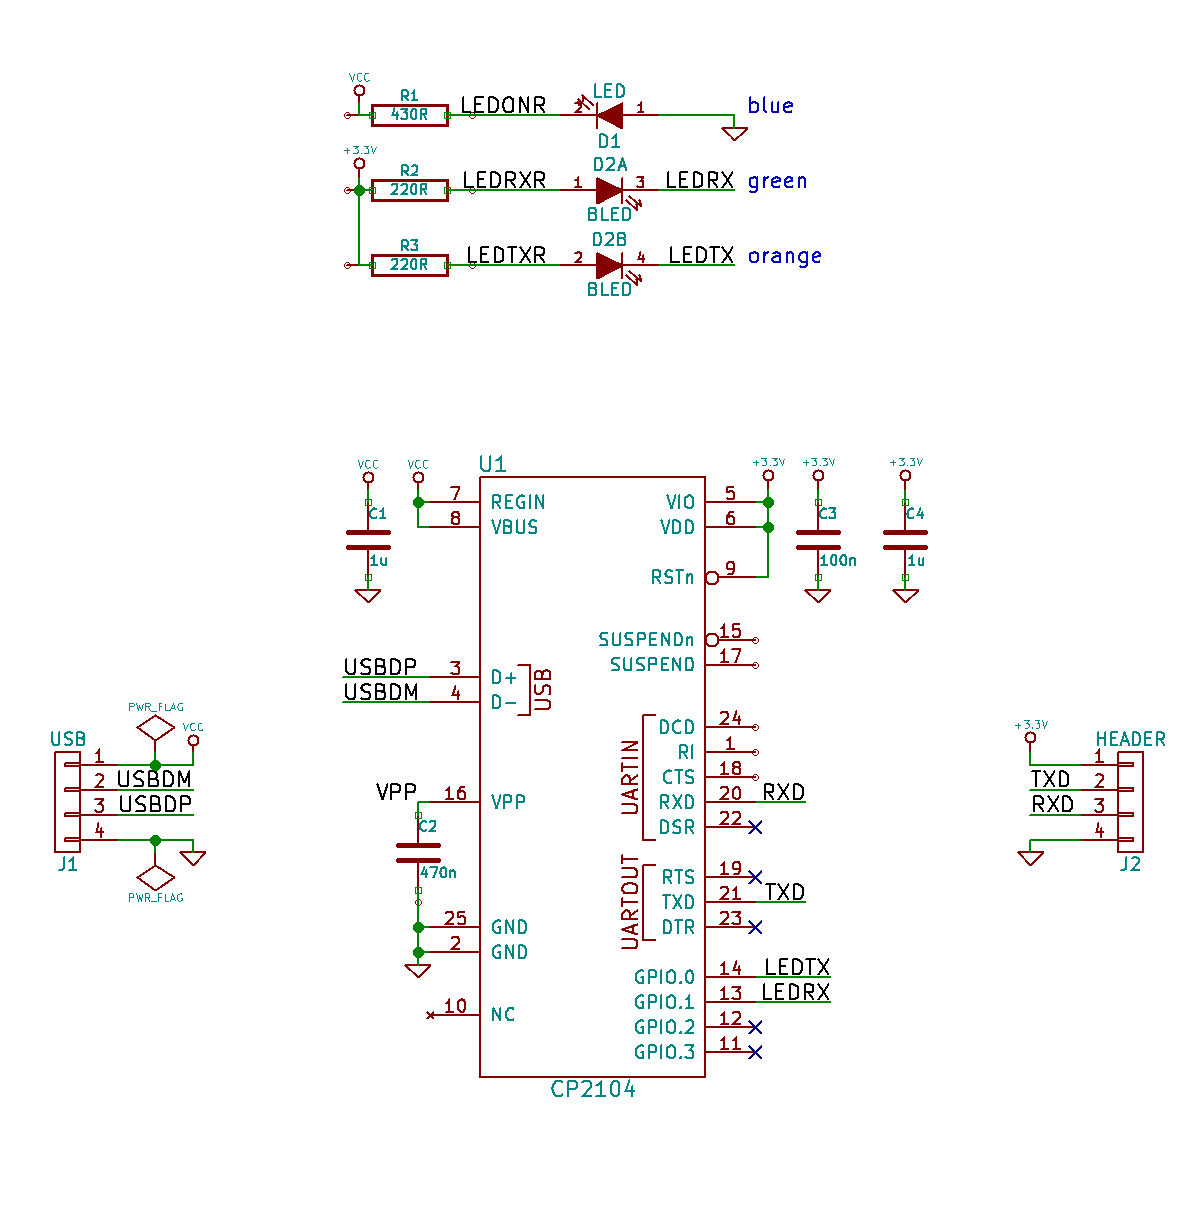
\includegraphics[width=.9\textwidth]{img/eesch-schem-final.png}
    \caption{Τελικό σχηματικό κύκλωμα της συσκευής}
    \label{fig:eesch-schem-final}
  \end{center}
\end{figure}

\begin{figure}
  \begin{center}
    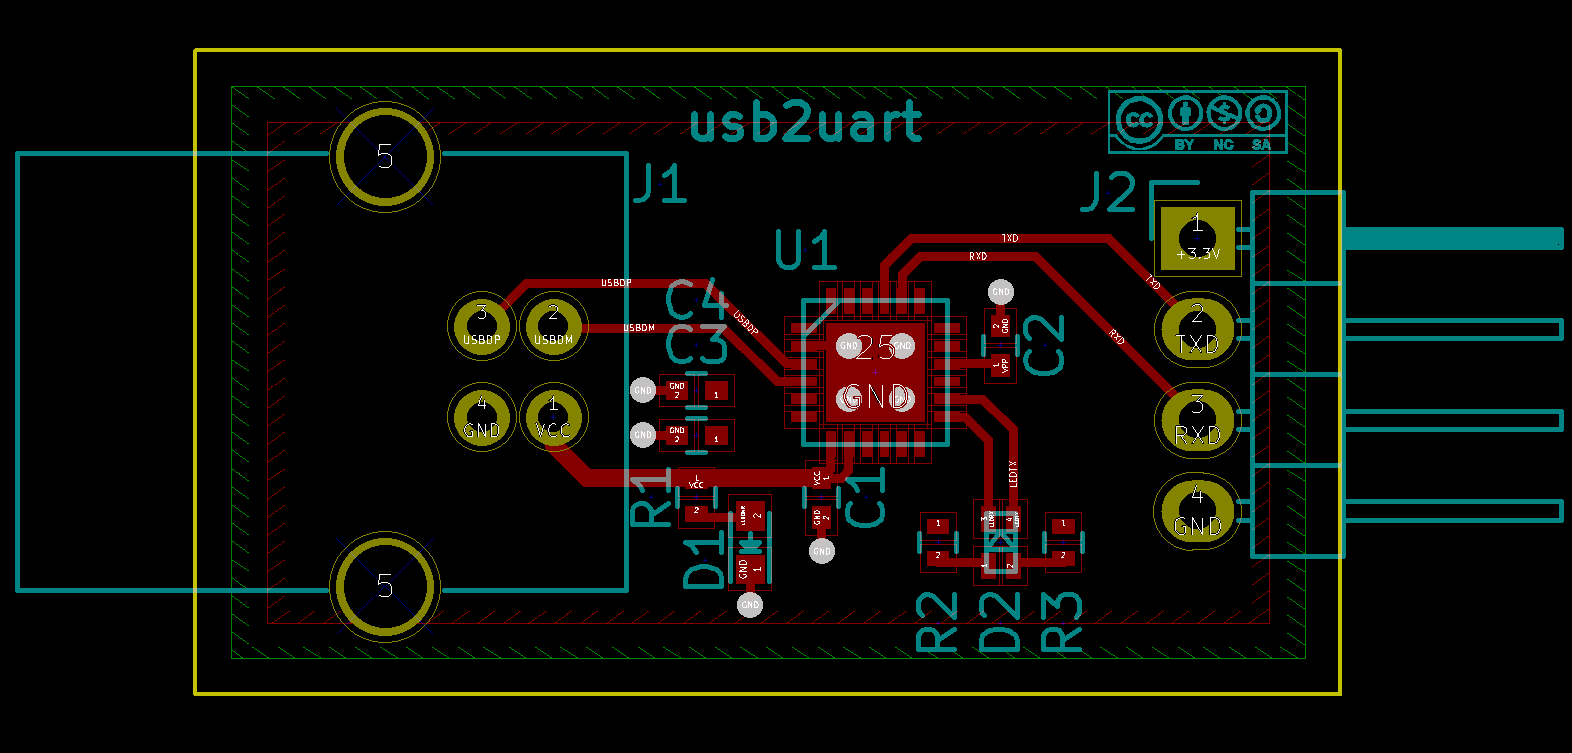
\includegraphics[width=.9\textwidth]{img/pcb-layout-final.png}
    \caption{Τελικό σχέδιο της πλακέτας της συσκευής}
    \label{fig:pcb-layout-final}
  \end{center}
\end{figure}

\subsection{Βασικές Έννοιες KiCad}

\subsubsection{Αρχεία KiCad}
Το \textenglish{KiCad} είναι μία ολοκληρωμένη σουίτα εφαρμογών σχεδίασης ηλεκτρονικών κυκλωμάτων \textenglish{EDA (Electronic Design Automation)}. Με το \textenglish{KiCad} είναι εφικτή η σχεδίαση σχηματικών και τυπωμένων ηλεκτρονικών κυκλωμάτων, χρησιμοποιώντας διαφορετικές εφαρμογές.

Τα σχηματικά κυκλώματα σχεδιάζονται στο \textenglish{KiCad} με την εφαρμογή \textenglish{EEschema}. Αποτελούνται από εξαρτήματα (για παράδειγμα ένας πυκνωτής ή ένα ολοκληρωμένο), συνδέσεις μεταξύ τους, και άλλα στοιχεία. Τα σχηματικά κυκλώματα είναι οργανωμένα σε σχηματικά φύλλα. Κάθε σχηματικό φύλλο αποτελεί και ένα αρχείο .sch στον υπολογιστή του χρήστη. Επίσης, η λίστα δικτύων κάθε κυκλώματος αποτελεί ένα αρχείο .net στον υπολογιστή του χρήστη.

Τα εξαρτήματα των σχηματικών μπορεί να ανήκουν σε μία βιβλιοθήκη του \textenglish{KiCad} ή μπορεί να τα έχει σχεδιάσει από το μηδέν ο χρήστης χρησιμοποιώντας τη σχετική εφαρμογή του \textenglish{KiCad} που ονομάζεται Επεξεργαστής Βιβλιοθήκης Εξαρτημάτων. Κάθε βιβλιοθήκη με εξαρτήματα αποτελεί και ένα αρχείο .lib στον υπολογιστή του χρήστη.

Τα τυπωμένα κυκλώματα σχεδιάζονται στο \textenglish{KiCad} με την εφαρμογή Pcbnew. Αποτελούνται από πλακέτες που περιέχουν αποτυπώματα εξαρτημάτων, συνδέσεις μεταξύ τους μέσω δρόμων, από τρύπες, via, κ.α.
Κάθε πλακέτα αποτελεί και ένα αρχείο .kicad\_pcb στον υπολογιστή του χρήστη. 

Τα τυπωμένα κυκλώματα απεικονίζονται και σε άλλα αρχεία που μπορεί να παράξει ο χρήστης με το \textenglish{KiCad}, και κυρίως αρχεία που χρησιμοποιούνται στην κατασκευή της πλακέτας. Τέτοια αρχεία είναι τα αρχεία gerber (.gtl, .gbl, .gtp, .gto, .gbs, .gts, .gbr, .gm1, κα), τα αρχεία διάτρησης (.drl), και τα αρχεία τοποθέτησης (.pos).

Τα αποτυπώματα εξαρτημάτων μπορεί να ανήκουν σε μία βιβλιοθήκη του \textenglish{KiCad} ή μπορεί να τα έχει σχεδιάσει από το μηδέν ο χρήστης χρησιμοποιώντας το σχετικό εργαλείο του \textenglish{KiCad}. Κάθε αποτύπωμα αποτελεί και ένα αρχείο .kicad\_mod στον υπολογιστή του χρήστη. Μία βιβλιοθήκη αποτυπωμάτων είναι ένας φάκελος αρχείων στον υπολογιστή του χρήστη, με επέκταση .pretty, ο οποίος φάκελος περιέχει αρχεία .kicad\_mod (ένα αρχείο .kicad\_mod για κάθε αποτύπωμα).

Τα αποτυπώματα μπορεί να έχουν τρισδιάστατη απεικόνιση ώστε ο χρήστης να μπορεί να απεικονίσει τρισδιάστατα το κύκλωμά του και να γνωρίζει πως θα είναι, πριν το κατασκευάσει. Το \textenglish{KiCad} προσφέρει τρισδιάστατες απεικονίσεις (3Δ σχήματα) για κάποια τυπικά εξαρτήματα, αλλά ο χρήστης να σχεδιάσει και τα δικά του 3Δ σχήματα από το μηδέν, με κάποιο πρόγραμμα τρισδιάστατης σχεδίασης. Κάθε τρισδιάστατη απεικόνιση αποτελεί και ένα αρχείο .wrl στον υπολογιστή του χρήστη. 

Κάθε εξάρτημα αντιστοιχεί και σε ένα αποτύπωμα (συνήθως πολλά εξαρτήματα έχουν το ίδιο αποτύπωμα). Αυτή η αντιστοίχηση αποτυπώματος-εξαρτήματος γίνεται από το εργαλείο \textenglish{Cvpcb}.

Το σύνολο του κυκλώματος (σχηματικό, πλακέτα) οργανώνεται από το \textenglish{KiCad} σε έργα. Κάθε έργο αποτελεί και ένα αρχείο .pro στον υπολογιστή του χρήστη. 

Τέλος, βοηθητικά, ο χρήστης συνίσταται να διατηρεί μαζί με τα αρχεία του κυκλώματος και όλα τα εγχειρίδια (ή τα φύλλα δεδομένων) των εξαρτημάτων που χρησιμοποιεί ώστε να μπορεί να αναφέρεται σε αυτά ως προς τις συνδέσεις που απαιτούν, τις έδρες που χρησιμοποιούν κα. Συνήθως κάθε εγχειρίδιο είναι συνήθως ένα αρχείο .pdf.

Όλα τα παραπάνω αρχεία (εξαρτήματα, αποτυπώματα, κυκλώματα, έργα, κοκ) καλό είναι να τα διατηρούμε στον ίδιο φάκελο αρχείων του υπολογιστή μας, για λόγους οργάνωσης.  

\subsubsection{Πλέγμα}
Mία πολύ χρήσιμη λειτουργία για τη σχεδίαση σε όλες τις εφαρμογές του \textenglish{KiCad} είναι ο ορισμός και η αλλαγή του πλέγματος το οποίο υπάρχει νοητά πάνω στην οθόνη μας μας και ορίζει τα σημεία όπου μπορεί να τοποθετηθεί ο δείκτης του ποντικιού. Πλέγμα 1mm σημαίνει ότι ο δείκτης του ποντικιού μπορεί να τοποθετηθεί σε διαστήματα του ενός mm αλλά όχι ενδιάμεσα. Το πλέγμα είναι βοηθητική, οπτική πληροφορία και δεν επηρεάζει με κανένα τρόπο τη λειτουργία του κυκλώματος. Για να αλλάξει το πλέγμα, κάνουμε δεξί κλικ σε κενό χώρο της κεντρικής οθόνης της εφαρμογής και επιλέγουμε Επιλογή Πλέγματος. Επίσης, μπορούμε να επιλέξουμε αν θα εμφανίζεται ή όχι μόνιμα το πλέγμα στην οθόνη μας, κάνοντας κλικ στο αντίστοιχο κουμπί στην αριστερή μπάρα λειτουργιών.

\subsubsection{Επιλογή λειτουργιών}
Όπως και στις περισσότερες εφαρμογές, έτσι και στο \textenglish{KiCad} και όλες τις εφαρμογές του, οι περισσότερες λειτουργίες μπορούν να εκτελεστούν με δύο τρόπους: είτε επιλέγοντας κάτι στο μενού είτε κάνοντας κλικ στο σχετικό κουμπί μίας μπάρας είτε κάνοντας δεξί κλικ και επιλέγοντας από το μενού του εμφανίζεται.

\newpage
\section{Δημιουργία έργου}
Εκτελέστε το πρόγραμμα \textenglish{KiCad}. Δείτε το κεφάλαιο \ref{sec:prereq} για την έκδοση του \textenglish{KiCad} που πρέπει να εκτελέσετε.

Θα εμφανιστεί η κεντρική οθόνη του προγράμματος \textenglish{KiCad} (σχήμα \ref{fig:kicad-main-window}). 

Αυτή αποτελείται από τα παρακάτω
\begin{itemize}
    \item γραμμή μενού και μπάρα βασικών λειτουργιών στο πάνω μέρος της οθόνης
    \item μπάρα για εκκίνηση βοηθητικών εφαρμογών στο πάνω δεξιά μέρος της οθόνης
    \item χώρο για εμφάνιση μηνυμάτων
    \item λίστα με τα αρχεία του έργου στο αριστερό μέρος της οθόνης
\end{itemize}

Από το μενού στο πάνω μέρος της οθόνης επιλέγουμε \textit{Αρχείο $\rightarrow$ Νέο Έργο $\rightarrow$ Νέο Έργο}. Δίνουμε στο νέο έργο (και το σχετικό αρχείο) ένα όνομα, προτείνεται το usb2uart, και το αποθηκεύουμε. Θα δημιουργηθούν τρία αρχεία στον υπολογιστή σας, τα usb2uart.pro, usb2uart.sch και usb2uart.kicad\_pcb για το έργο, το σχηματικό, και την πλακέτα αντίστοιχα.

Προτείνεται να δημιουργηθεί το έργο σε έναν φάκελο του υπολογιστή σας ο οποίος θα είναι αφιερωμένος στο συγκεκριμένο έργο και θα περιέχει όλα τα αρχεία του έργου, και μόνο αυτά.

\begin{figure}
  \begin{center}
    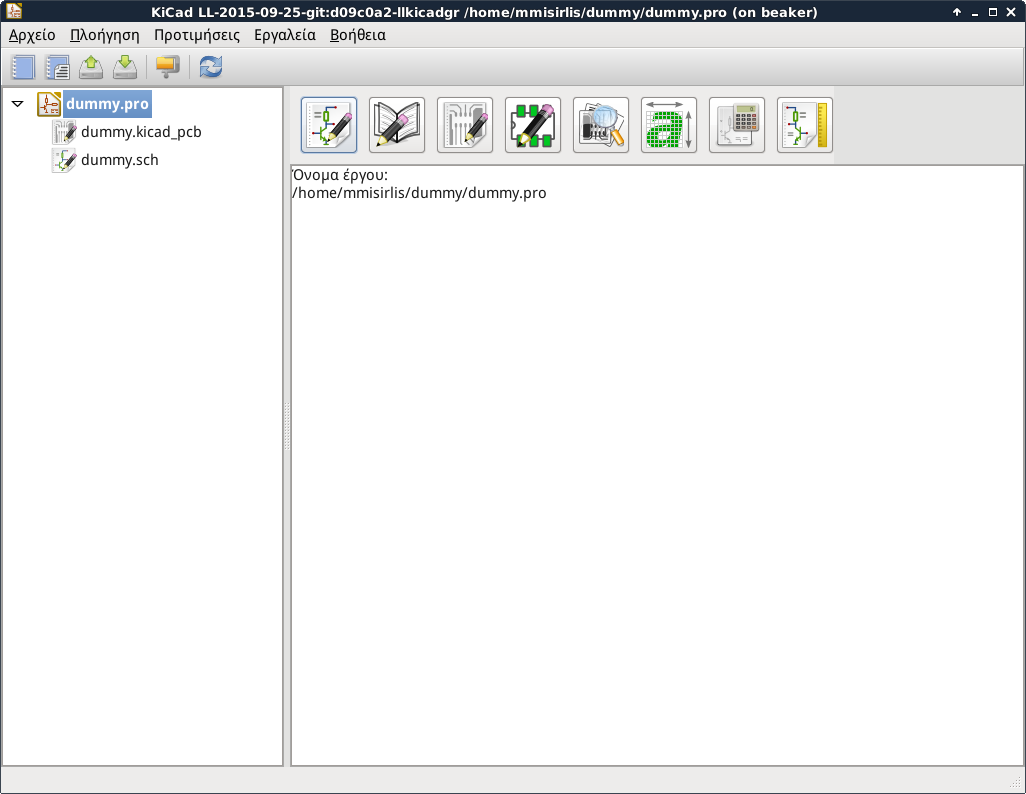
\includegraphics[width=.9\textwidth]{img/kicad-main-window.png}
    \caption{Κεντρική οθόνη του προγράμματος KiCad}
    \label{fig:kicad-main-window}
  \end{center}
\end{figure}

\newpage
\section{Σχεδίαση Σχηματικού Κυκλώματος}

\subsection{Δημιουργία σχηματικού}

\subsubsection{\textenglish{Εφαρμογή EEschema} }
Από το μενού στο πάνω μέρος της κεντρικής οθόνης του \textenglish{KiCad} επιλέγουμε \textit{Εργαλεία $\rightarrow$ Εκτέλεση \textenglish{EEschema}}, για να εκτελεστεί η εφαρμογή \textenglish{EEschema} με την οποία σχεδιάζουμε το σχηματικό κύκλωμα. 

Θα εμφανιστεί στην οθόνη σας η κεντρική οθόνη της εφαρμογής \textenglish{EEschema} (σχήμα \ref{fig:eesch-main-window}). Αυτή αποτελείται από τα παρακάτω
\begin{itemize}
    \item ένα φύλλο σχηματικού κυκλώματος στο κέντρο της οθόνης, όπου θα σχεδιάσουμε το κύκλωμα
    \item γραμμή μενού στο πάνω μέρος της οθόνης, με όλες σχεδόν τις δυνατές λειτουργίες
    \item μπάρα βασικών λειτουργιών στο πάνω μέρος της οθόνης
    \item μπάρα με γενικές λειτουργίες στο αριστερό μέρος της οθόνης, όπως για εμφάνιση ή όχι του πλέγματος, χρήση mm ή ιντσών, κα
    \item μπάρα με συγκεκριμένες λειτουργίες σχεδίασης στο δεξί μέρος της οθόνης, όπως σχεδίαση δρόμων, τοποθέτηση εξαρτημάτων, σχεδίαση γραφικών, κα
    \item μπάρα κατάστασης στο κάτω μέρος της οθόνης με πληροφορίες συντεταγμένων, ενεργού εξαρτήματος, κα
\end{itemize}

\begin{figure}
  \begin{center}
    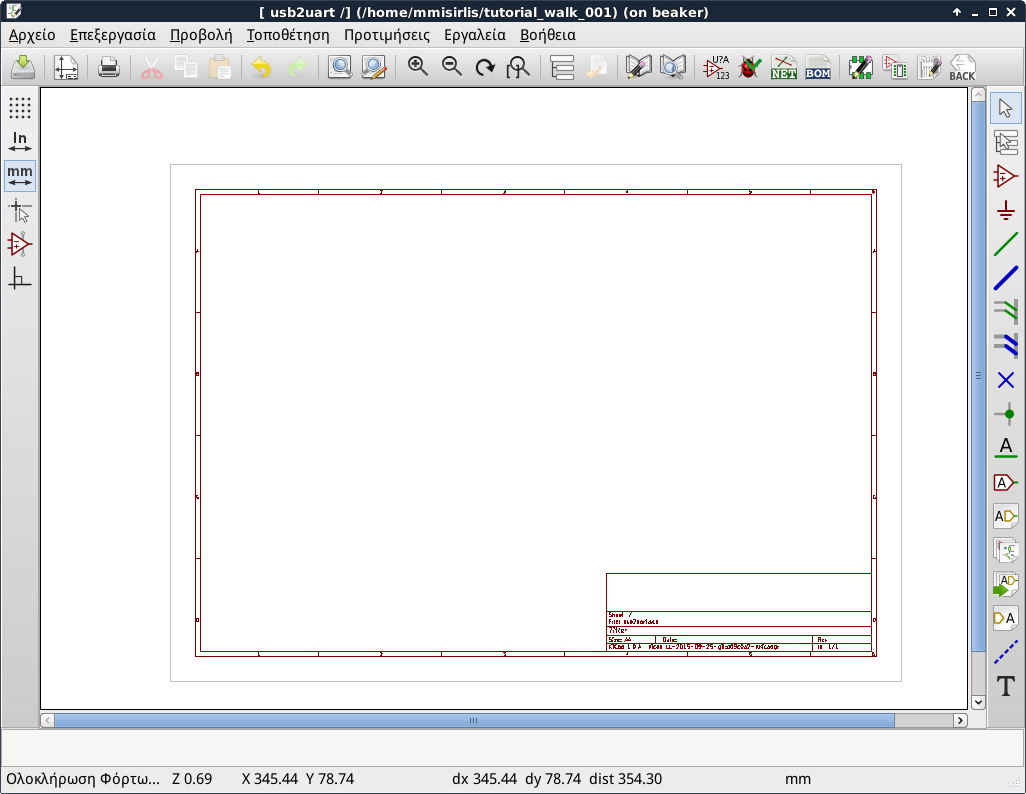
\includegraphics[width=.9\textwidth]{img/eesch-main-window.png}
    \caption{Κεντρική οθόνη της εφαρμογής \textenglish{EEschema}}
    \label{fig:eesch-main-window}
  \end{center}
\end{figure}

Το \textenglish{EEschema} μπορεί να σχεδιάσει κυκλώματα που αποτελούνται από πολλά σχηματικά φύλλα. Σε αυτό το tutorial το κύκλωμά μας αποτελείται από ένα και μοναδικό φύλλο.

\subsubsection{Ρυθμίσεις σελίδας}
Αρχικά θα ορίσουμε τις ρυθμίσεις σελίδας. Από το μενού στο πάνω μέρος της οθόνης του \textenglish{EEschema} επιλέξτε \textit{Αρχείο $\rightarrow$ Ρυθμίσεις Σελίδας}. Στο παράθυρο που εμφανίζεται (σχήμα \ref{fig:eesch-dial-pagesett}), ορίστε τις ρυθμίσεις της σελίδας σας, όπως μέγεθος χαρτιού, ημερομηνία έκδοσης, τίτλος κυκλώματος, και πατήστε ΟΚ. Αυτές οι ρυθμίσεις δεν έχουν κάποια ηλεκτρική ή λειτουργική σημασία για το κύκλωμα, είναι όμως χρήσιμες πληροφορίες για την οργάνωση των κυκλωμάτων σας. Προτείνεται να ορίσετε μόνο την ημερομηνία έκδοσης, την αναθεώρηση και τον τίτλο.

\begin{figure}
  \begin{center}
    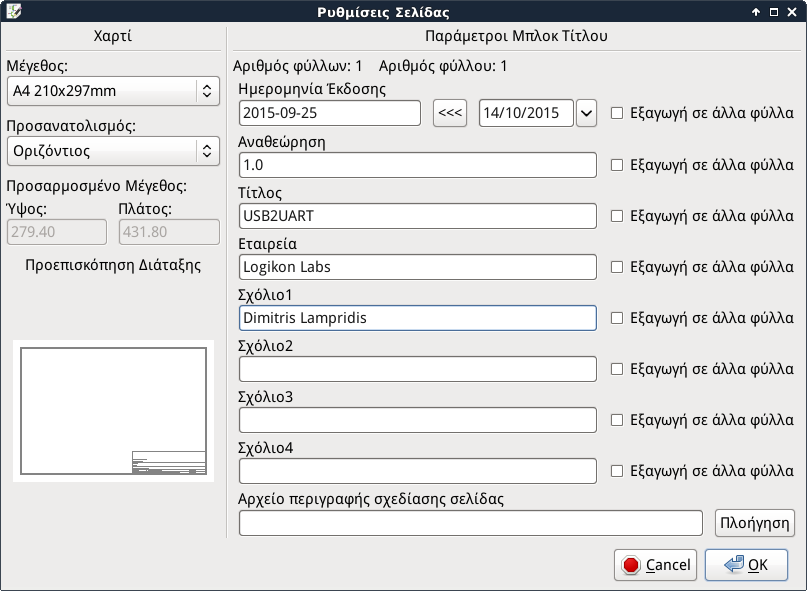
\includegraphics[width=.5\textwidth]{img/eesch-dial-pagesett.png}
    \caption{Ρυθμίσεις Σελίδας \textenglish{EEschema}}
    \label{fig:eesch-dial-pagesett}
  \end{center}
\end{figure}

\subsubsection{Σχεδίαση γραφικών}

Στη συνέχεια θα σχεδιάσουμε κάποιες βοηθητικές γραμμές στο σχηματικό μας.

Από το μενού στο πάνω μέρος της οθόνης του \textenglish{EEschema} επιλέξτε \textit{Τοποθέτηση $\rightarrow$ Γραφικό Πολυγραμμής}.

Με αυτό το εργαλείο μπορείτε να σχεδιάσετε γραμμές στο φύλλο σας. Αυτές οι γραμμές γραφικών δεν έχουν κάποια ηλεκτρική ή λειτουργική σημασία για το κύκλωμα, είναι απλή ζωγραφική, είναι όμως χρήσιμες για την οργάνωση των κυκλωμάτων σας.

Σχεδιάστε στο φύλλο μία κατακόρυφη γραμμή που χωρίζει το φύλλο σε δύο τμήματα (σχήμα \ref{fig:eesch-main-lines}). Το δεξί τμήμα πρέπει να είναι περίπου το ένα τρίτο του συνολικού φύλλου. Αυτό το δεξί τμήμα θα το χρησιμοποιήσουμε ως χώρο για να γράφουμε  βοηθητικές πληροφορίες (όπως η τρέχουσα έκδοση του κυκλώματος), και για να εναποθέτουμε προσωρινά τα εξαρτήματα πριν τα τοποθετήσουμε στην οριστική τους θέση στο αριστερό τμήμα της σελίδας.

\begin{figure}
  \begin{center}
    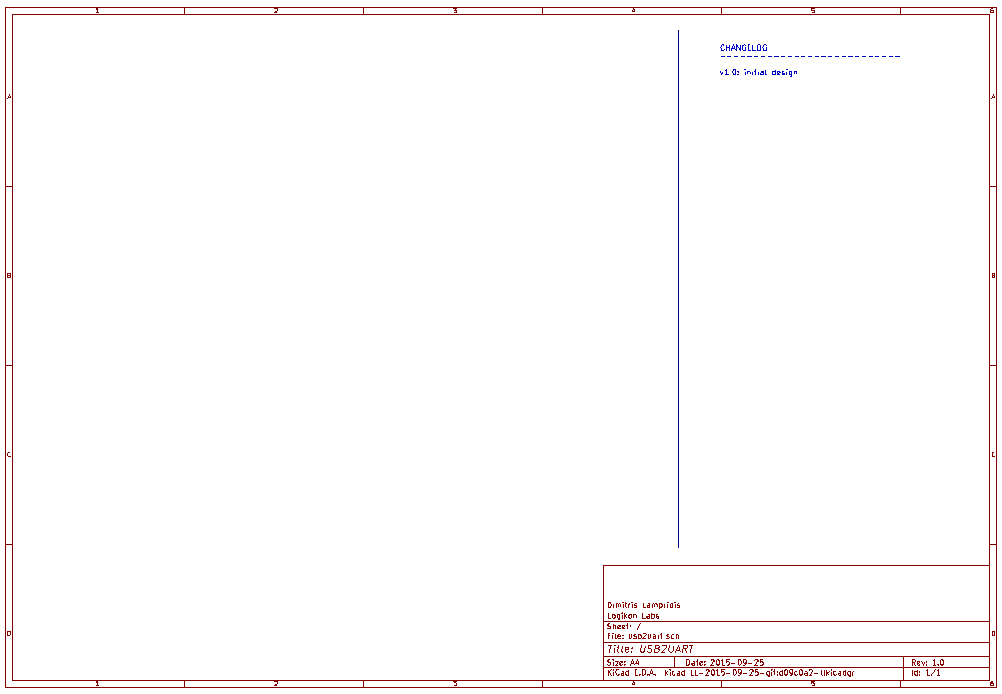
\includegraphics[width=.9\textwidth]{img/eesch-main-lines.png}
    \caption{Σχηματικό φύλλο χωρισμένο στα δύο}
    \label{fig:eesch-main-lines}
  \end{center}
\end{figure}

\subsubsection{Βιβλιοθήκες εξαρτημάτων}

Η εφαρμογή \textenglish{EEschema} περιλαμβάνει πολλά εξαρτήματα, τα οποία μπορείτε να χρησιμοποιήσετε στα κυκλώματά σας. Τα εξαρτήματα αυτά είναι οργανωμένα σε βιβλιοθήκες. Το \textenglish{EEschema} περιλαμβάνει αρχικά περίπου 30 βιβλιοθήκες οι οποίες περιλαμβάνονται εξαρχής σε κάθε νέο έργο που δημιουργείται. Για λόγους απλότητας του έργου μας, εμείς θα αφαιρέσουμε τις βιβλιοθήκες εξαρτημάτων που δεν έχουν εξαρτήματα χρήσιμα για το συγκεκριμένο κύκλωμα που σχεδιάζουμε.

Από το μενού στο πάνω μέρος της οθόνης του \textenglish{EEschema} επιλέξτε \textit{Προτιμήσεις $\rightarrow$ Βιβλιοθήκες Εξαρτημάτων}. Θα εμφανιστεί ένα παράθυρο με τις βιβλιοθήκες του έργου. Σε αυτό το παράθυρο επιλέξτε όλες τις βιβλιοθήκες (μία προς μία ή όλες μαζί) εκτός από τις βιβλιοθήκες power, device και conn και κάντε κλικ στο Αφαίρεση. Θα πρέπει στο παράθυρο να φαίνονται μόνο οι τρεις βιβλιοθήκες power, device και conn (σχήμα \ref{fig:eesch-dial-libr}). 

Κάντε κλικ στο ΟΚ για να επανέλθετε στην κεντρική οθόνη.

Από το μενού στο πάνω μέρος της οθόνης του \textenglish{EEschema} επιλέξτε \textit{Αρχείο $\rightarrow$ Αποθήκευση Σχηματικού Έργου}.

\begin{figure}
  \begin{center}
    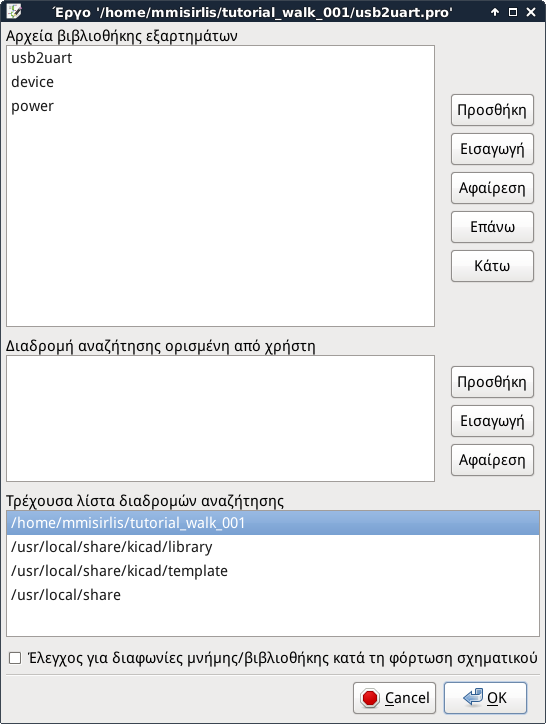
\includegraphics[width=.5\textwidth]{img/eesch-dial-libr.png}
    \caption{Παράθυρο με τις βιβλιοθήκες του έργου}
    \label{fig:eesch-dial-libr}
  \end{center}
\end{figure}

%Σε αυτό το σημείο αντιστοιχούν τα αρχεία από το αρχείο kicad\_tut00.zip.

\subsection{Προσθήκη εξαρτημάτων}

\subsubsection{Προσθήκη βασικών εξαρτημάτων}

Εφόσον έχουμε δημιουργήσει και ρυθμίσει το φύλλο μας, πρέπει να προσθέσουμε τα εξαρτήματα που θα αποτελέσουν το κύκλωμά μας. Πρέπει να βρισκόμαστε στην κεντρική οθόνη της εφαρμογής \textenglish{EEschema}.

Από το μενού στο πάνω μέρος της οθόνης του \textenglish{EEschema} επιλέξτε \textit{Τοποθέτηση $\rightarrow$ Εξάρτημα} και κάντε κλικ στο δεξί τμήμα του φύλλου σας. Θα εμφανιστεί ένα παράθυρο επιλογής εξαρτήματος (σχήμα \ref{fig:eesch-dial-addcomp}).

\begin{figure}
  \begin{center}
    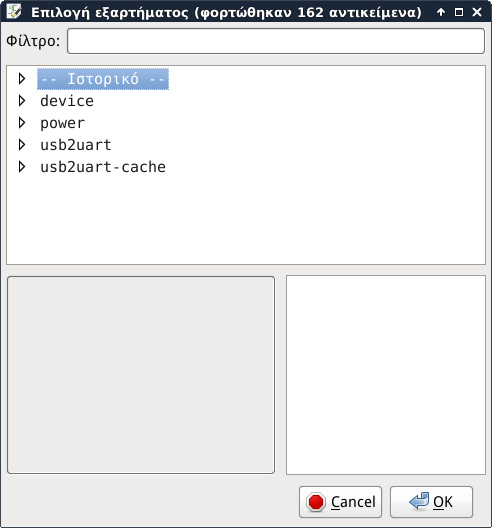
\includegraphics[width=.5\textwidth]{img/eesch-dial-addcomp.png}
    \caption{Παράθυρο επιλογής εξαρτήματος}
    \label{fig:eesch-dial-addcomp}
  \end{center}
\end{figure}

Στο παράθυρο επιλογής εξαρτήματος επιλέξτε το εξάρτημα με όνομα C (ένας πυκνωτής) από τη βιβλιοθήκη device, πατήστε ΟΚ (θα επανέλθετε το φύλλο σχηματικού) και κάντε κλικ στο δεξί τμήμα του φύλλου σας ώστε να τοποθετηθεί στο φύλλο το εξάρτημα που επιλέξατε. 

Αφού τοποθετήσετε το εξάρτημα με όνομα C στο φύλλο, ακολουθήστε την ίδια διαδικασία ώστε να τοποθετήσετε στο φύλλο σας (στο δεξί τμήμα) όλα τα παρακάτω εξαρτήματα. 

\begin{itemize}
    \item R, από τη βιβλιοθήκη device
    \item LED, από τη βιβλιοθήκη device
    \item VCC, από τη βιβλιοθήκη power
    \item +3.3V, από τη βιβλιοθήκη power
    \item GND, από τη βιβλιοθήκη power
    \item CONN\_01X04, από τη βιβλιοθήκη conn
\end{itemize}

Με την ολοκλήρωση αυτών των τοποθετήσεων, έχουμε στο φύλλο μας 7 εξαρτήματα, τοποθετημένα όλα τακτοποιημένα στο δεξί τμήμα του φύλλου (σχήμα \ref{fig:eesch-circ-placedccomp}).

\begin{figure}
  \begin{center}
    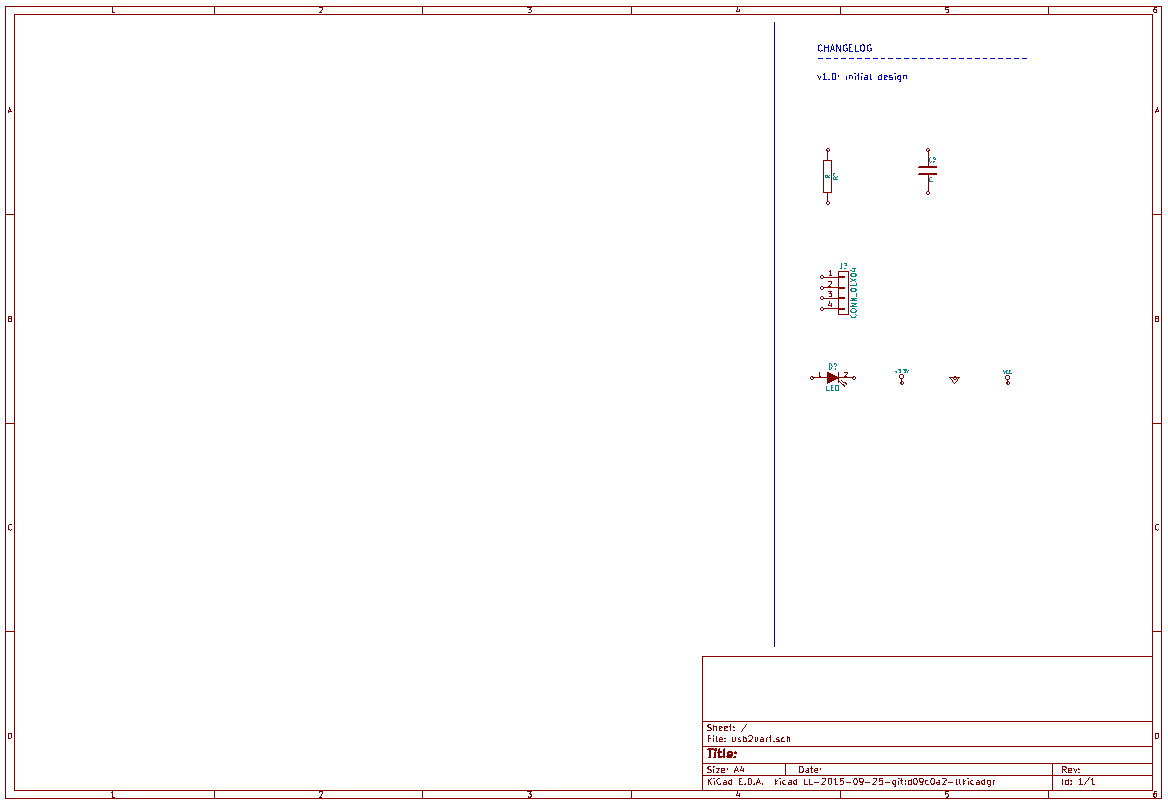
\includegraphics[width=.9\textwidth]{img/eesch-circ-placedccomp.png}
    \caption{Φύλλο σχηματικού με τοποθετημένα 7 εξαρτήματα}
    \label{fig:eesch-circ-placedccomp}
  \end{center}
\end{figure}

\subsubsection{Ιδιότητες εξαρτημάτων}

Για λόγους ευκολίας ανάγνωση του κυκλώματος, θα χρειαστεί να αλλάξουμε το πρόθεμα της ονομασίας αναφοράς του CONN\_01X04 από P σε J. Για να το κάνουμε αυτό πρέπει να κάνουμε δεξί κλικ πάνω στο εξάρτημα CONN\_01X04, και από το μενού που εμφανίζεται να επιλέξουμε \textit{Επεξεργασία Εξαρτήματος $\rightarrow$ Επεξεργασία}. Αυτό θα μας εμφανίσει το παράθυρο Ιδιότητες Εξαρτήματος (σχήμα \ref{fig:eesch-dial-compprop}), όπου πρέπει να ορίσουμε την Τιμή Πεδίου της Ονομασίας Αναφοράς να είναι J? και όχι P?.

\begin{figure}
  \begin{center}
    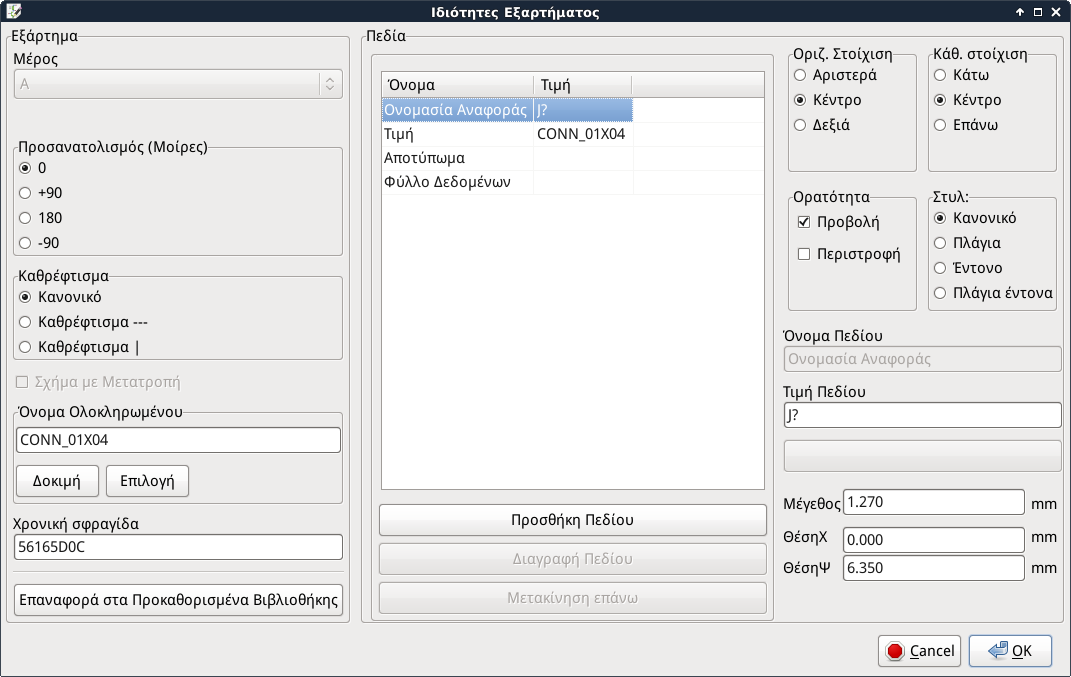
\includegraphics[width=.5\textwidth]{img/eesch-dial-compprop.png}
    \caption{Παράθυρο Ιδιότητες Εξαρτήματος}
    \label{fig:eesch-dial-compprop}
  \end{center}
\end{figure}

\subsubsection{Αντίγραφα εξαρτημάτων}

Στη συνέχεια θα χρειαστεί να τοποθετήσουμε στο κύκλωμά μας και άλλα εξαρτήματα C, R και CONN\_01X04. Για να το κάνουμε αυτό, αντί να κάνουμε πάλι τοποθέτηση και να τα επιλέγουμε από τις βιβλιοθήκες, μπορούμε να κάνουμε αντιγραφή των εξαρτημάτων που ήδη έχουμε στο φύλλο μας. 

Για να αντιγράψουμε (δηλαδή να φτιάξουμε ακόμα ένα αντίγραφο) ενός εξαρτήματος πρέπει να κάνουμε δεξί κλικ πάνω στο εξάρτημα, από το μενού που εμφανίζεται να επιλέξουμε \textit{Αντιγραφή Εξαρτήματος}, και μετά να κάνουμε κλικ πάνω στο φύλλο εκεί όπου θέλουμε να φτιαχτεί το αντίγραφο του εξαρτήματος. 

Με αυτό τον τρόπο πρέπει να φτιάξουμε τα παρακάτω εξαρτήματα.

\begin{itemize}
    \item 3 αντίγραφα του C, ώστε να έχουμε συνολικά 4 C στο φύλλο
    \item 2 αντίγραφα του R, ώστε να έχουμε συνολικά 3 R στο φύλλο
    \item 1 αντίγραφο του CONN\_01X04, ώστε να έχουμε συνολικά 2 CONN\_01X04 στο φύλλο
\end{itemize}

Με την ολοκλήρωση αυτών των τοποθετήσεων έχουμε στο φύλλο μας 13 εξαρτήματα (σχήμα \ref{fig:eesch-circ-placedccompcop}), τοποθετημένα όλα τακτοποιημένα στο δεξί τμήμα του φύλλου.

\begin{figure}
  \begin{center}
    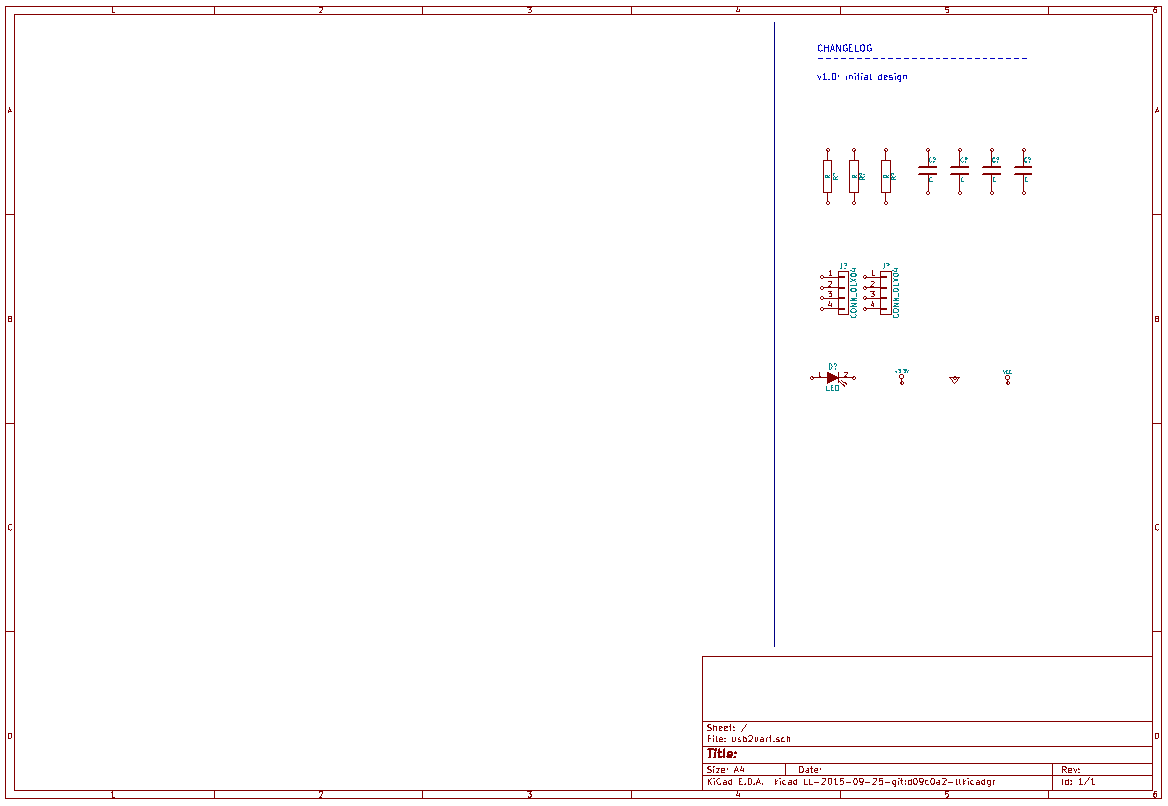
\includegraphics[width=.9\textwidth]{img/eesch-circ-placedccompcop.png}
    \caption{Φύλλο σχηματικού με τοποθετημένα 13 εξαρτήματα}
    \label{fig:eesch-circ-placedccompcop}
  \end{center}
\end{figure}

%Σε αυτό το σημείο αντιστοιχούν τα αρχεία από το αρχείο kicad\_tut01.zip.

\subsection{Δημιουργία εξαρτημάτων}
Το \textenglish{EEschema} μας δίνει τη δυνατότητα να επεξεργαστούμε ένα υπάρχον εξάρτημα ή και να δημιουργήσουμε ένα εξάρτημα από το μηδέν.

\subsubsection{Επεξεργαστής Βιβλιοθήκης Εξαρτημάτων}

Εμείς σε αυτή τη φάση θέλουμε να εντάξουμε στο σχηματικό κύκλωμα το ολοκληρωμένο CP2104. Το \textenglish{KiCad} όμως δεν έχει στις βιβλιοθήκες του εξάρτημα που να αντιστοιχεί στο ολοκληρωμένο CP2104, οπότε θα το δημιουργήσουμε.

Από το μενού στο πάνω μέρος της οθόνης του \textenglish{EEschema} επιλέξτε \textit{Εργαλεία $\rightarrow$ Επεξεργαστής Βιβλιοθήκης}.

Θα εμφανιστεί στην οθόνη σας η κεντρική οθόνη του Επεξεργαστή Βιβλιοθήκης Εξαρτημάτων (σχήμα \ref{fig:libed-main-window}). Αυτή αποτελείται από τα παρακάτω
\begin{itemize}
    \item έναν κενό χώρο στο κέντρο της οθόνης, όπου θα σχεδιάσουμε το εξάρτημα
    \item γραμμή μενού στο πάνω μέρος της οθόνης, με όλες σχεδόν τις δυνατές λειτουργίες
    \item μπάρα βασικών λειτουργιών στο πάνω μέρος της οθόνης
    \item μπάρα με γενικές λειτουργίες στο αριστερό μέρος της οθόνης
    \item μπάρα με συγκεκριμένες λειτουργίες σχεδίασης στο δεξί μέρος της οθόνης, όπως τοποθέτηση ακροδεκτών, γραφικών, κα
    \item μπάρα κατάστασης στο κάτω μέρος της οθόνης με πληροφορίες συντεταγμένων, ενεργού εξαρτήματος, κα
\end{itemize}

Στον κενό χώρο στο κέντρο της οθόνης θα σχεδιάσουμε το σώμα του εξαρτήματος, θα προσθέσουμε ακροδέκτες, θα γράψουμε το όνομά του, κλπ. Όλα αυτά τα στοιχεία αφού τα προσθέσουμε στο σώμα του εξαρτήματος, μπορούμε να τα επιλέγουμε με δεξί κλικ του ποντικιού και να τα επεξεργαζόμαστε- κυρίως να τα μετακινούμε και να τα περιστρέφουμε.

\begin{figure}
  \begin{center}
    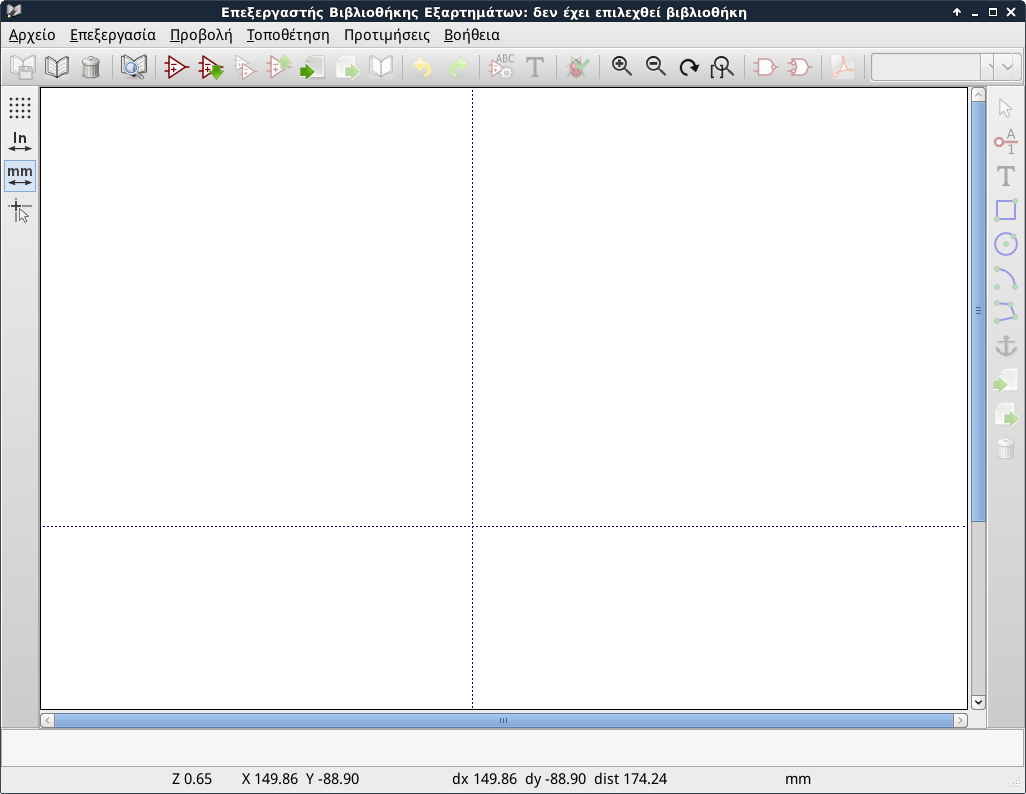
\includegraphics[width=.9\textwidth]{img/libed-main-window.png}
    \caption{Kεντρική σελίδα - Επεξεργαστής Βιβλιοθήκης Εξαρτημάτων}
    \label{fig:libed-main-window}
  \end{center}
\end{figure}

\subsubsection{Δημιουργία νέου εξαρτήματος}

Αρχικά θα δημιουργήσουμε ένα νέο εξάρτημα.

Κάντε κλικ στο εικονίδιο \textit{Δημιουργία νέου εξαρτήματος} στην πάνω μπάρα 
\includegraphics[scale=.5]{img/libed-ico-newcomp.png}. 

Θα εμφανιστεί το παράθυρο Ιδιότητες Εξαρτήματος (σχήμα \ref{fig:libed-dial-newcompprop}). Στο παράθυρο αυτό, στο Όνομα εξαρτήματος γράψτε το όνομα CP2104, αφήστε όλες τις υπόλοιπες επιλογές στις προκαθορισμένες ρυθμίσεις, και επιλέξτε ΟΚ.

\begin{figure}
  \begin{center}
    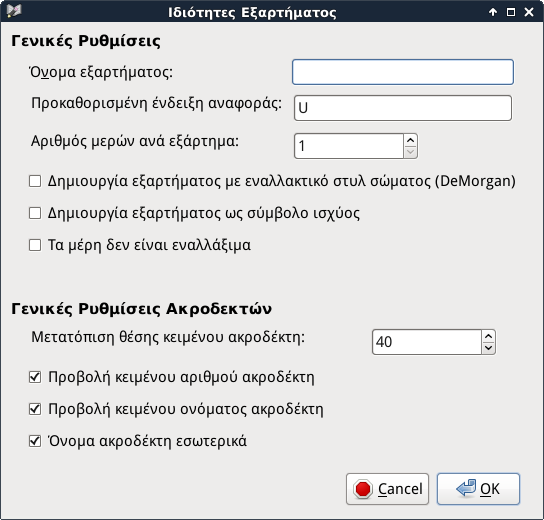
\includegraphics[width=.5\textwidth]{img/libed-dial-newcompprop.png}
    \caption{Παράθυρο Ιδιότητες Εξαρτήματος για νέο εξάρτημα}
    \label{fig:libed-dial-newcompprop}
  \end{center}
\end{figure}

Πλέον έχουμε δημιουργήσει ένα νέο εξάρτημα, χωρίς κανέναν ακροδέκτη. 

\subsubsection{Δημιουργία νέας βιβλιοθήκης εξαρτημάτων}

Πρέπει να δημιουργήσουμε μία νέα βιβλιοθήκη, να αποθηκεύσουμε το νέο εξάρτημα σε αυτήν, και να εντάξουμε τη βιβλιοθήκη στο έργο μας.

Από την μπάρα στο πάνω μέρος της οθόνης επιλέξτε Αποθήκευση τρέχοντος εξαρτήματος σε νέα βιβλιοθήκη 
\includegraphics[scale=.5]{img/libed-ico-savnewlib.png}.

Αυτό θα εμφανίσει ένα παράθυρο όπου θα πρέπει να δώσετε το όνομα της νέας βιβλιοθήκης που θέλετε να δημιουργήσετε ώστε να μπει σε αυτή το νέο εξάρτημα. Το όνομα της βιβλιοθήκης θα είναι και το όνομα του αρχείου στον υπολογιστή σας, το οποίο θα περιέχει τη βιβλιοθήκη. 

Δώστε στη βιβλιοθήκη το όνομα \textenglish{usb2uart.lib} και αποθηκεύστε την στον υπολογιστή σας, στον ίδιο φάκελο με το υπόλοιπο έργο.

Θα εμφανιστεί ένα μήνυμα που θα λέει ότι η βιβλιοθήκη πρέπει να δηλωθεί στο \textenglish{EEschema} για να χρησιμοποιηθεί. Πατήστε ΟΚ.

Κλείστε τον Επεξεργαστή Βιβλιοθήκης Εξαρτημάτων, εκτελέστε το \textenglish{EEschema} (αν δεν τρέχει ήδη) και από το μενού στο πάνω μέρος της οθόνης του \textenglish{EEschema} επιλέξτε \textit{Προτιμήσεις $\rightarrow$ Βιβλιοθήκες Εξαρτημάτων}. Θα εμφανιστεί ένα παράθυρο με τις βιβλιοθήκες του έργου. 

Σε αυτό το παράθυρο πατήστε Προσθήκη, βρείτε στο σύστημα αρχείων του υπολογιστή σας το αρχείο της βιβλιοθήκης που δημιουργήσατε προηγουμένως, και ανοίξτε το. Η βιβλιοθήκη usb2uart θα πρέπει να έχει προστεθεί στις βιβλιοθήκες του έργου σας (σχήμα \ref{fig:libed-dial-libs}). Πατήστε ΟΚ στο παράθυρο με τις βιβλιοθήκες του έργου.

\begin{figure}
  \begin{center}
    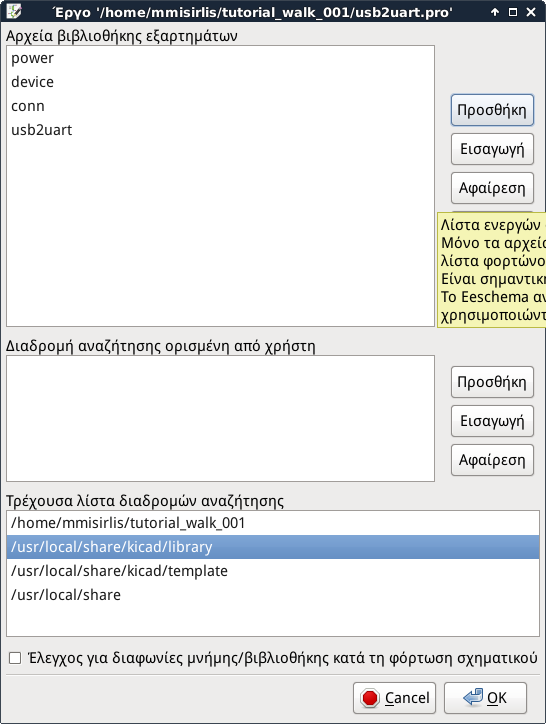
\includegraphics[width=.5\textwidth]{img/libed-dial-libs.png}
    \caption{Παράθυρο με τις βιβλιοθήκες του έργου (έχει προστεθεί η usb2uart)}
    \label{fig:libed-dial-libs}
  \end{center}
\end{figure}

Από το μενού στο πάνω μέρος της οθόνης του \textenglish{EEschema} επιλέξτε \textit{Αρχείο $\rightarrow$ Αποθήκευση Σχηματικού Έργου}.

\subsubsection{Φόρτωση εξαρτήματος}
Τώρα πρέπει να φορτώσουμε το νέο εξάρτημα, από τη βιβλιοθήκη όπου το αποθηκεύσαμε, ώστε να το επεξεργαστούμε.

Από το μενού στο πάνω μέρος της οθόνης του \textenglish{EEschema} επιλέξτε \textit{Εργαλεία $\rightarrow$ Επεξεργαστής Βιβλιοθήκης} για να συνεχίσετε να δουλεύετε στον Επεξεργαστή Βιβλιοθήκης.

Κάντε κλικ στο εικονίδιο \textit{Επιλογή βιβλιοθήκης εργασίας} 
\includegraphics[scale=.5]{img/libed-ico-selnewlib.png} στην πάνω μπάρα, και στο παράθυρο που εμφανίζεται (σχήμα \ref{fig:libed-dial-libsel}) επιλέξτε τη βιβλιοθήκη usb2uart, και πατήστε ΟΚ, ώστε να επιστρέψετε στην κεντρική οθόνη του Επεξεργαστή Βιβλιοθήκης. 

Στον τίτλο του παραθύρου πρέπει να φαίνεται το όνομα της βιβλιοθήκης που επιλέξατε.

\begin{figure}
  \begin{center}
    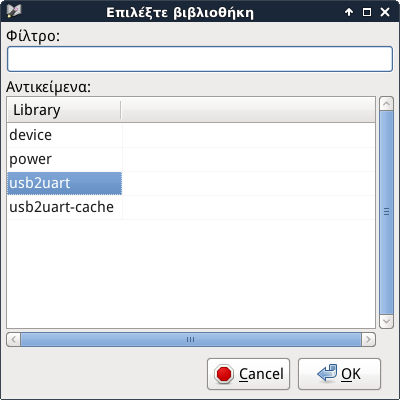
\includegraphics[width=.5\textwidth]{img/libed-dial-libsel.png}
    \caption{Παράθυρο επιλογής βιβλιοθήκης εργασίας}
    \label{fig:libed-dial-libsel}
  \end{center}
\end{figure}

Τώρα πρέπει, στην κεντρική οθόνη του Επεξεργαστή Βιβλιοθήκης, να φορτώσουμε το εξάρτημα το οποίο θέλουμε να επεξεργαστούμε. 

Κάντε κλικ στο εικονίδιο \textit{Φόρτωση εξαρτήματος για επεξεργασία από την τρέχουσα βιβλιοθήκη} 
\includegraphics[scale=.5]{img/libed-ico-loadcomp.png}. Στο παράθυρο επιλογής εξαρτήματος που θα εμφανιστεί επιλέξτε το εξάρτημα με όνομα CP2104 από τη βιβλιοθήκη usb2uart, και πατήστε ΟΚ. Θα επανέλθετε στην κεντρική οθόνη του Επεξεργαστή Βιβλιοθήκης και θα έχει φορτωθεί στην οθόνη το εξάρτημα CP2104 (το οποίο σε αυτή τη φάση είναι απλά ένα όνομα).

\subsubsection{Ορισμός ιδιοτήτων εξαρτήματος}

Στη συνέχεια θα ορίσουμε κάποιες από τις γενικές ιδιότητες του εξαρτήματος. 

Κάντε κλικ στο εικονίδιο \textit{Επεξεργασία ιδιοτήτων εξαρτήματος} 
\includegraphics[scale=.5]{img/libed-ico-compprop.png} 
για να εμφανιστεί το παράθυρο Ιδιοτήτων για το εξάρτημα (σχήμα \ref{fig:libed-dial-compprop}). 

\begin{figure}
  \begin{center}
    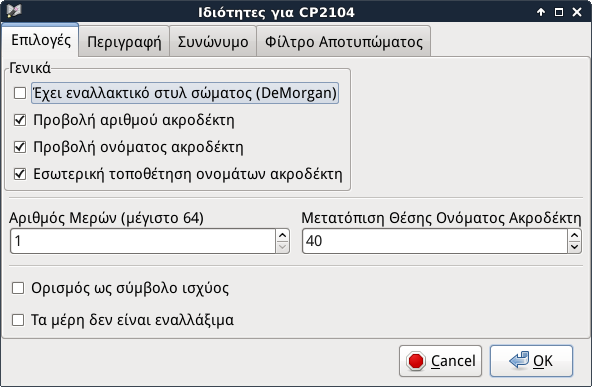
\includegraphics[width=.5\textwidth]{img/libed-dial-compprop.png}
    \caption{Παράθυρο Ιδιοτήτων για το εξάρτημα CP2104}
    \label{fig:libed-dial-compprop}
  \end{center}
\end{figure}

Σε αυτό το παράθυρο συμπληρώστε τα παρακάτω πεδία και μετά πατήστε ΟΚ για να επιστρέψετε στην κεντρική οθόνη του Επεξεργαστή Βιβλιοθήκης.

\begin{itemize}
    \item Περιγραφή: CP2104 Μετατροπέας USB-σε-UART
    \item Φίλτρο αποτυπώματος: QFN
    \item (προαιρετικά) όνομα του αρχείου τεκμηρίωσης ή του εγχειρίδιου για το εξάρτημα, αν το έχετε
\end{itemize}

\subsubsection{Σχεδίαση σώματος εξαρτήματος}
Τώρα πρέπει να σχεδιάσουμε αρχικά το σώμα του εξαρτήματος. Βρισκόμαστε στην κεντρική οθόνη του Επεξεργαστή Βιβλιοθήκης.

Από το μενού στο πάνω μέρος της οθόνης επιλέξετε \textit{Τοποθέτηση $\rightarrow$ Ορθογώνιο} και σχεδιάστε στην οθόνη ένα κατακόρυφο ορθογώνιο όπως φαίνεται στη σχετική εικόνα (σχήμα \ref{fig:libed-circ-body}). Για να σχεδιάσετε, κάντε κλικ εκεί που θέλετε να είναι η πάνω αριστερή γωνία και μετά ένα ακόμα κλικ εκεί που θέλετε να είναι η κάτω δεξιά γωνία του σχεδίου.

Στο εξάρτημα πρέπει να εμφανίζονται το όνομά του (CP2104) και η ονομασία αναφοράς (U?). Κάντε δεξί κλικ επάνω στο όνομα, επιλέξτε μετακίνηση, και τοποθετήστε το όνομα κάτω από το σώμα του εξαρτήματος. Επίσης κάντε δεξί κλικ επάνω στην ονομασία αναφοράς, επιλέξτε μετακίνηση, και τοποθετήστε την πάνω από το σώμα του εξαρτήματος (σχήμα \ref{fig:libed-circ-body}). 

\begin{figure}
  \begin{center}
    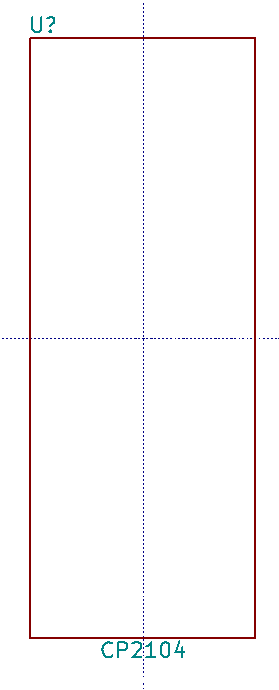
\includegraphics[width=.2\textwidth]{img/libed-circ-body.png}
    \caption{Ορθογώνιο σώμα εξαρτήματος, με τοποθετημένα όνομα και αναφορά}
    \label{fig:libed-circ-body}
  \end{center}
\end{figure}

Να σημειωθεί ότι έως τώρα έχουμε ορίσει μόνο βοηθητικά στοιχεία του εξαρτήματος: το όνομά του, τι φίλτρο αποτυπώματος θα έχει, πως θα εμφανίζεται στο σχηματικό, κα. Τίποτα από αυτά δεν έχει ηλεκτρική ή λειτουργική σημασία για το εξάρτημα.

\subsubsection{Προσθήκη ακροδεκτών εξαρτήματος}

Τώρα πρέπει να προσθέσουμε τους ακροδέκτες που θα αποτελούν το εξάρτημά μας. Το πόσους και τι είδους ακροδέκτες πρέπει να προσθέσουμε θα το γνωρίζουμε από το εγχειρίδιο του ολοκληρωμένου. Αυτό μπορείτε να το βρείτε στην ιστοσελίδα του κατασκευαστή του ολοκληρωμένου. 

Κατά τη συγγραφή αυτού του οδηγού εκμάθησης το εγχειρίδιο του CP2104 (έκδοση/Rev. 1.1) βρισκόταν στον παρακάτω σύνδεσμο:\\
\href{https://www.silabs.com/Support\%20Documents/TechnicalDocs/cp2104.pdf}{https://www.silabs.com/Support\%20Documents/TechnicalDocs/cp2104.pdf}. 

Αν δεν είναι διαθέσιμο σε αυτό τον σύνδεσμο επισκεφθείτε τη σελίδα του κατασκευαστή και αναζητήστε εκεί το εγχειρίδιο του CP2104: \\
\href{https://www.silabs.com/}{https://www.silabs.com/}

Με βάση το εγχειρίδιο του CP2104, πρέπει να ορίσουμε 25 ακροδέκτες: τους 24 τυπικούς ακροδέκτες, και επιπλέον θα έχουμε ως ακροδέκτη και την θερμική έδρα GND του CP2104. Οπότε συνολικά θα έχουμε 25 ακροδέκτες για το CP2104.

Σε αυτό το tutorial θα ορίσουμε 2 ακροδέκτες μόνο, και οι υπόλοιποι πρέπει να προστεθούν από εσάς, κατά τον ίδιο τρόπο όπως και οι 2 πρώτοι, ορίζοντας πάντα τις σωστές ιδιότητες για κάθε ακροδέκτη, με βάση το εγχειρίδιο. Εναλλακτικά μπορείτε να πάρετε έτοιμο το εξάρτημα, με σχεδιασμένους όλους τους ακροδέκτες, από τα αρχεία του tutorial.

\paragraph{Προσθήκη ακροδέκτη Vio}

Αρχικά ας προσθέσουμε τον ακροδέκτη Vio, ο οποίος σύμφωνα με το εγχειρίδιο έχει το όνομα Vio, του έχει αποδοθεί ο αριθμός 5, και η λειτουργία του είναι είσοδος ισχύος τροφοδοσίας.

Από το μενού στο πάνω μέρος της οθόνης επιλέξετε \textit{Τοποθέτηση $\rightarrow$ Ακροδέκτης} και κάντε κλικ στην κεντρική οθόνη για να εμφανιστεί το παράθυρο Ιδιότητες Ακροδέκτη (σχήμα \ref{fig:libed-dial-viocompprop}).

\begin{figure}
  \begin{center}
    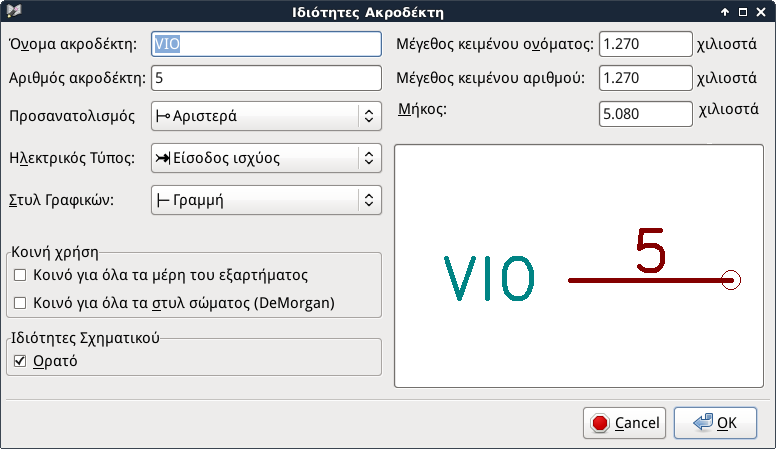
\includegraphics[width=.5\textwidth]{img/libed-dial-viocompprop.png}
    \caption{Παράθυρο Ιδιότητες Ακροδέκτη για τον Vio του CP2104}
    \label{fig:libed-dial-viocompprop}
  \end{center}
\end{figure}

Σε αυτό το παράθυρο πρέπει να ορίσουμε τις παρακάτω σημαντικές ιδιότητες για τον ακροδέκτη.

\begin{itemize}
    \item Όνομα ακροδέκτη: Vio
    \item Αριθμός ακροδέκτη: 5
    \item Προσανατολισμός: Αριστερά
    \item Ηλεκτρικός Τύπος: Είσοδος ισχύος
\end{itemize}

Αφού ορίσουμε τα παραπάνω , επιλέγουμε ΟΚ και μετά πρέπει να τοποθετήσουμε τον ακροδέκτη στο σώμα του εξαρτήματος. Προτείνεται να τοποθετηθεί στο πάνω δεξιά μέρος του σώματος (σχήμα \ref{fig:libed-circ-vioplaced}).

\begin{figure}
  \begin{center}
    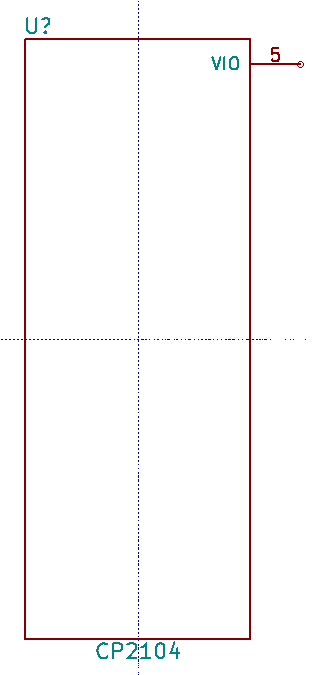
\includegraphics[width=.2\textwidth]{img/libed-circ-vioplaced.png}
    \caption{Σώμα εξαρτήματος, με τοποθετημένο έναν ακροδέκτη}
    \label{fig:libed-circ-vioplaced}
  \end{center}
\end{figure}

Να σημειωθεί ότι δεν έχει ηλεκτρική σημασία σε ποιο σημείο του σώματος θα τοποθετήσουμε τον ακροδέκτη (πάνω αριστερά, στη μέση κλπ) ή τι προσανατολισμό θα του δώσουμε. Η θέση και ο προσανατολισμός απλά μας βοηθούν στην απεικόνιση του σχηματικού. Συνήθως τους ακροδέκτες που έχουν συναφή λειτουργία τους σχεδιάζουμε κοντά τον έναν στον άλλο.

Αυτά που έχουν ηλεκτρική σημασία είναι το όνομα, ο αριθμός, και ο τύπος του ακροδέκτη, καθώς λαμβάνονται υπόψιν κατά τον Έλεγχο Ηλεκτρικών Κανόνων που θα κάνουμε με το \textenglish{KiCad} αργότερα.

\paragraph{Προσθήκη ακροδέκτη D+}

Στη συνέχεια προσθέσετε τον ακροδέκτη D+, ο οποίος σύμφωνα με το εγχειρίδιο έχει το όνομα D+, του έχει αποδοθεί ο αριθμός 3, και η λειτουργία του είναι είσοδος/έξοδος δεδομένων.

Όπως και πριν, από το μενού στο πάνω μέρος της οθόνης επιλέξετε \textit{Τοποθέτηση $\rightarrow$ Ακροδέκτης} και κάντε κλικ στην κεντρική οθόνη για να εμφανιστεί το παράθυρο Ιδιότητες Ακροδέκτη.

Σε αυτό το παράθυρο πρέπει να ορίσουμε τις παρακάτω σημαντικές ιδιότητες για τον ακροδέκτη, και μετά να τον τοποθετήσουμε στο σώμα του εξαρτήματος. Προτείνεται να τοποθετηθεί στο κεντρικό, αριστερό μέρος του σώματος \ref{fig:libed-circ-twopinslaced}.

\begin{itemize}
    \item Όνομα ακροδέκτη: D+
    \item Αριθμός ακροδέκτη: 3
    \item Προσανατολισμός: Δεξιά
    \item Ηλεκτρικός Τύπος: Αμφίδρομο
\end{itemize}

\begin{figure}
  \begin{center}
    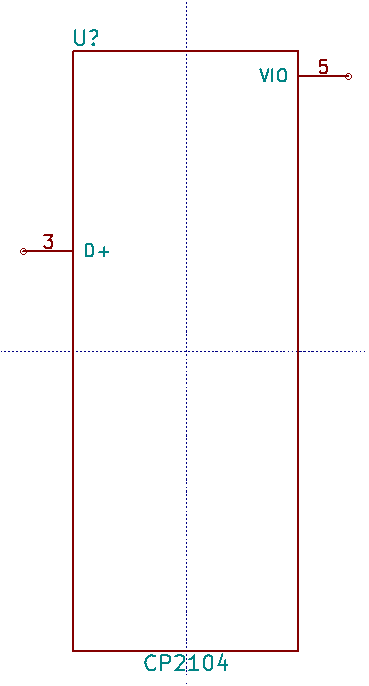
\includegraphics[width=.2\textwidth]{img/libed-circ-twopinslaced.png}
    \caption{Σώμα εξαρτήματος, με τοποθετημένους δύο ακροδέκτες}
    \label{fig:libed-circ-twopinslaced}
  \end{center}
\end{figure}

Συνεχίζοντας κατά τον ίδιο τρόπο, τοποθετήστε και τους υπόλοιπους 23 ακροδέκτες του εξαρτήματος, ώστε να καταλήξετε τελικά σε ένα εξάρτημα με 25 ακροδέκτες (σχήμα \ref{fig:libed-circ-allpinslaced}), όπως ορίζει το εγχειρίδιό του.

\begin{figure}
  \begin{center}
    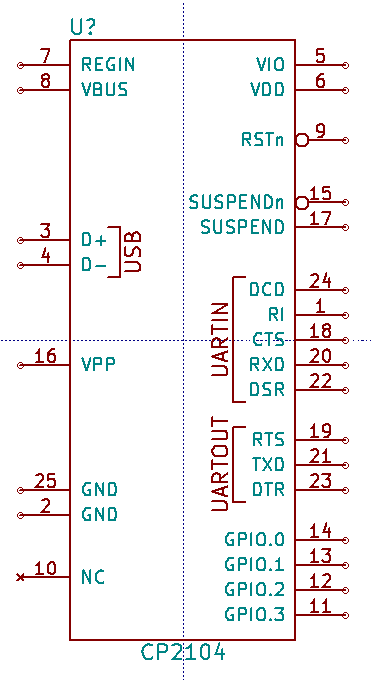
\includegraphics[width=.35\textwidth]{img/libed-circ-allpinslaced.png}
    \caption{Σώμα εξαρτήματος, με τοποθετημένους όλους τους ακροδέκτες}
    \label{fig:libed-circ-allpinslaced}
  \end{center}
\end{figure}

\subsubsection{Προσθήκη κειμένων και γραφικών}

Στο εξάρτημα, εκτός από το σχεδιασμό του περιγράμματος και την τοποθέτηση των ακροδεκτών, μπορούμε να τοποθετήσουμε και άλλες οπτικές πληροφορίες, όπως κείμενο και επιπλέον γραμμές γραφικών που να προσφέρουν βοηθητικές πληροφορίες. Αυτές οι πληροφορίες φαίνονται και στο σχήμα \ref{fig:libed-circ-allpinslaced}.

Για να προσθέσουμε κείμενο, επιλέγουμε από τη δεξιά μπάρα το το εικονίδιο \textit{Προσθήκη κειμένου στο σώμα εξαρτήματος} 
\includegraphics[scale=.5]{img/libed-ico-text.png}
, κάνουμε κλικ στο σώμα του εξαρτήματος, και στο παράθυρο Ιδιότητες Κειμένου Βιβλιοθήκης \label{fig:libed-dial-text} που εμφανίζεται γράφουμε ό,τι κείμενο θέλουμε, επιλέγουμε αν θα εμφανίζεται κάθετα, τι στοίχιση θα έχει, κοκ.

\begin{figure}
  \begin{center}
    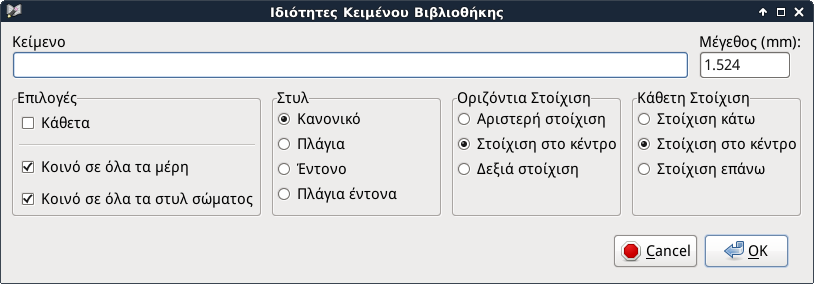
\includegraphics[width=.5\textwidth]{img/libed-dial-text.png}
    \caption{Παράθυρο Ιδιότητες Κειμένου Βιβλιοθήκης}
    \label{fig:libed-dial-text}
  \end{center}
\end{figure}

Για παράδειγμα, στο CP2104 μπορούμε να βάλουμε κατακόρυφα δίπλα στους ακροδέκτες D+ και D- τη λέξη USB, το οποίο θα μας βοηθάει να θυμόμαστε ότι αυτή είναι η λειτουργία τους.

Επίσης, μπορούμε να βάλουμε κατακόρυφα δίπλα στους ακροδέκτες RTX, TXD, DTR τη λέξη UARTOUT, το οποίο θα μας βοηθάει να θυμόμαστε ότι αυτή είναι η λειτουργία τους.

Ομοίως και για τους ακροδέκτες DCD, RI, CTS, RXD, DSR τη λέξη UARTΙΝ.

Αφού έχουμε ορίσει όλους τους ακροδέκτες και έχουμε οριστικοποιήσει τη μορφή του εξαρτήματος, θα πρέπει να αποθηκεύσουμε το εξάρτημα στη βιβλιοθήκη. Αποθηκεύστε την εργασία σας επιλέγοντας από το μενού στο πάνω μέρος της οθόνης \textit{Αρχείο $\rightarrow$ Αποθήκευση της τρέχουσας βιβλιοθήκης}. Θα εμφανιστούν δύο παράθυρα που θα ζητούν την επιβεβαίωση της αποθήκευσης. Επιλέξτε καταφατικά και στα δύο.

Πλέον έχουμε ολοκληρώσει τη δημιουργία του εξαρτήματος και το έχουμε αποθηκεύσει στη βιβλιοθήκη μας.

%Σε αυτό το σημείο αντιστοιχούν τα αρχεία από το αρχείο kicad\_tut02.zip.

\subsection{Εξαρτημάτα με πολλά μέρη}

Σε αυτό το κεφάλαιο θα φορτώσουμε ένα εξάρτημα (ένα LED) από μία εσωτερική βιβλιοθήκη του \textenglish{KiCad}, θα το επεξεργαστούμε κάνοντάς το να αποτελείται από πολλά μέρη, και θα το αποθηκεύσουμε, αλλαγμένο, σε μία δική μας βιβλιοθήκη.

Όταν ένα εξάρτημα αποτελείται από πολλά μέρη στο \textenglish{KiCad}, αυτό σημαίνει ότι το εξάρτημα είναι ένα φυσικό αντικείμενο (πχ ένα ολοκληρωμένο) το οποίο όμως αποτελείται εσωτερικά από πολλά ίδια μέρη. Στην περίπτωσή μας, εμείς θέλουμε ένα εξάρτημα το οποίο αποτελείται από δύο LED.

Δεν υπάρχει εξάρτημα το οποίο αποτελείται από δύο LED στις γνωστές βιβλιοθήκες του \textenglish{KiCad}. Θα πρέπει να το σχεδιάσουμε εμείς.

Θα μπορούσαμε να δημιουργήσουμε από το μηδέν ένα νέο τέτοιο εξάρτημα, στον Επεξεργαστή Βιβλιοθήκης Εξαρτημάτων. 

Είναι όμως καλύτερα να χρησιμοποιήσουμε το υπάρχον εξάρτημα LED, και να σχεδιάσουμε ένα νέο εξάρτημα το οποίο θα αποτελείται από δύο LED.

\subsubsection{Φόρτωση εξαρτήματος}
Θεωρούμε ότι είμαστε στην αρχική οθόνη του \textenglish{KiCad}. 

Από το μενού στο πάνω μέρος της οθόνης επιλέξτε \textit{Εργαλεία $\rightarrow$ Εκτέλεση Επεξεργαστή Βιβλιοθήκης}, ώστε να φορτωθεί η κεντρική οθόνη του Επεξεργαστή Βιβλιοθήκης Εξαρτημάτων.

Από την πάνω μπάρα, επιλέξτε το κουμπί Επιλογή βιβλιοθήκης εργασίας και στο παράθυρο που θα εμφανιστεί κάντε κλικ πάνω στη βιβλιοθήκη device και πατήστε ΟΚ για να φορτωθεί η βιβλιοθήκη και να επιστρέψετε στην κεντρική οθόνη του Επεξεργαστή Βιβλιοθήκης Εξαρτημάτων.

Από την κεντρική οθόνη του Επεξεργαστή Βιβλιοθήκης Εξαρτημάτων κάντε κλικ στο εικονίδιο \textit{Φόρτωση εξαρτήματος για επεξεργασία από την τρέχουσα βιβλιοθήκη} 
\includegraphics[scale=.5]{img/libed-ico-loadcomp.png}
. Το παράθυρο που θα εμφανιστεί εμφανίζει όλα τα εξαρτήματα της βιβλιοθήκης LED. Βρείτε στη λίστα το εξάρτημα LED, επιλέξτε το, και πατήστε ΟΚ για να φορτωθεί στην κεντρική οθόνη του Επεξεργαστή Βιβλιοθήκης Εξαρτημάτων (σχήμα \ref{fig:libed-wind-led}).

\begin{figure}
  \begin{center}
    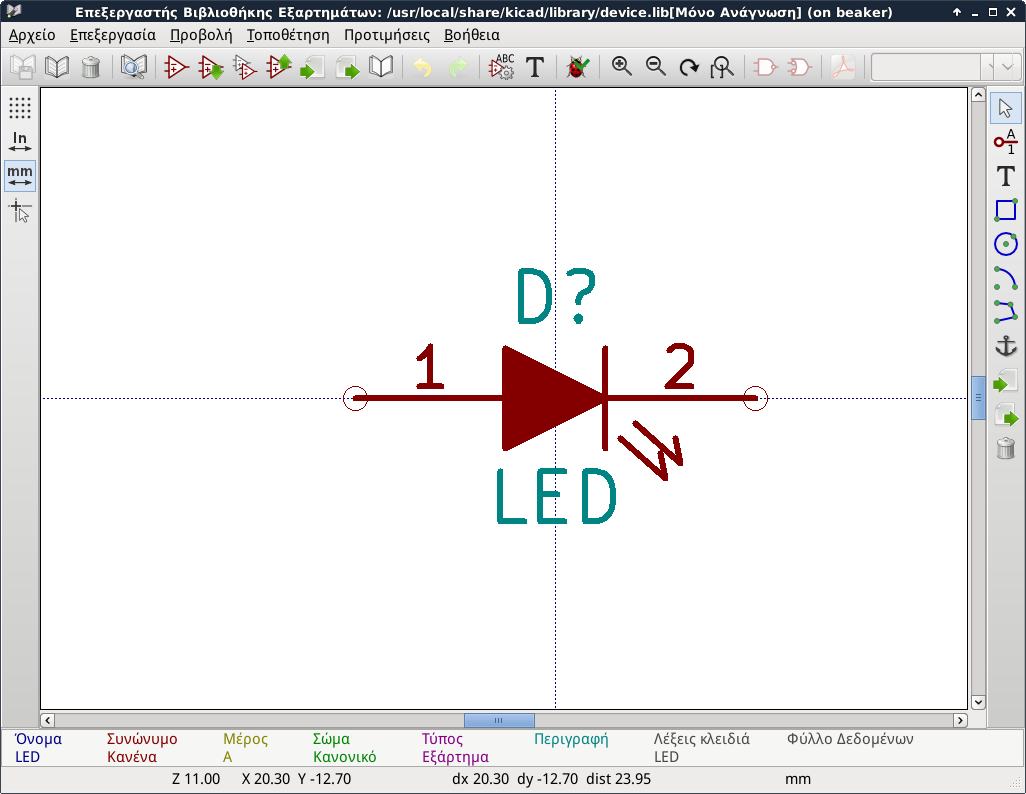
\includegraphics[width=.9\textwidth]{img/libed-wind-led.png}
    \caption{Κεντρική οθόνη του Επεξεργαστή Βιβλιοθήκης Εξαρτημάτων με φορτωμένο το εξάρτημα LED}
    \label{fig:libed-wind-led}
  \end{center}
\end{figure}

Τώρα, αφού έχουμε φορτώσει το εξάρτημα, θα φτιάξουμε ένα αντίγραφό του, και το αντίγραφο θα το αλλάξουμε ώστε να καλύπτει τις ανάγκες μας.

\subsubsection{Δημιουργία αντίγραφου εξαρτήματος}

Από την κεντρική οθόνη του Επεξεργαστή Βιβλιοθήκης Εξαρτημάτων κάντε κλικ στο εικονίδιο \textit{Δημιουργία νέου εξαρτήματος από το τρέχον} 
\includegraphics[scale=.5]{img/libed-ico-copycomp.png}
. Θα εμφανιστεί το παράθυρο Όνομα Εξαρτήματος (σχήμα \ref{fig:libed-dial-compname}). Ονομάστε το νέο εξάρτημα bLED και πατήστε ΟΚ.

\begin{figure}
  \begin{center}
    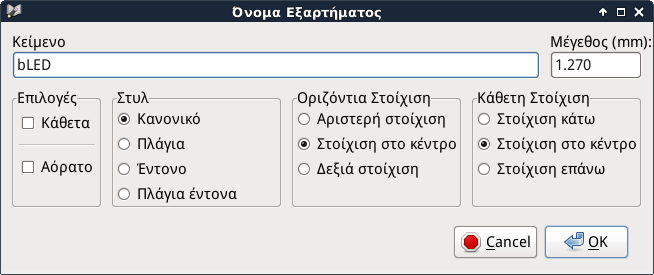
\includegraphics[width=.5\textwidth]{img/libed-dial-compname.png}
    \caption{Παράθυρο Όνομα Εξαρτήματος}
    \label{fig:libed-dial-compname}
  \end{center}
\end{figure}

Πλέον έχουμε δημιουργήσει ένα νέο εξάρτημα, το οποίο καλό είναι να αποθηκεύσουμε. Αλλά βρισκόμαστε στη βιβλιοθήκη device, η οποία επειδή είναι εσωτερική βιβλιοθήκη του \textenglish{KiCad} δεν μπορούμε να γράψουμε σε αυτήν. Αυτό φαίνεται και από τον τίτλο του παραθύρου όπου εμφανίζεται το κείμενο Μόνο Ανάγνωση.

Πρέπει να αποθηκεύσουμε το εξάρτημά μας σε άλλη βιβλιοθήκη.

Από την πάνω μπάρα, επιλέξτε το κουμπί Επιλογή βιβλιοθήκης εργασίας 
\includegraphics[scale=.5]{img/libed-ico-selnewlib.png}
και στο παράθυρο που θα εμφανιστεί κάντε κλικ πάνω στη βιβλιοθήκη usb2uart και πατήστε ΟΚ για να φορτωθεί η βιβλιοθήκη και να επιστρέψετε στην κεντρική οθόνη του Επεξεργαστή Βιβλιοθήκης Εξαρτημάτων.

Αποθηκεύστε την εργασία σας επιλέγοντας από το μενού στο πάνω μέρος της οθόνης \textit{Αρχείο $\rightarrow$ Αποθήκευση της τρέχουσας βιβλιοθήκης}. Θα εμφανιστούν δύο παράθυρα που θα ζητούν την επιβεβαίωση αυτή της αποθήκευσης. Επιλέξτε καταφατικά και στα δύο.

Πλέον έχουμε αποθηκεύσει στη δική μας βιβλιοθήκη το εξάρτημα που φτιάξαμε.

\subsubsection{Αλλαγή ιδιοτήτων εξαρτήματος}
Κάντε κλικ στο εικονίδιο \textit{Επεξεργασία ιδιοτήτων εξαρτήματος} 
\includegraphics[scale=.5]{img/libed-ico-compprop.png} 
για να εμφανιστεί το παράθυρο Ιδιοτήτων για το εξάρτημα (σχήμα \ref{fig:libed-dial-bledprop}). 

\begin{figure}
  \begin{center}
    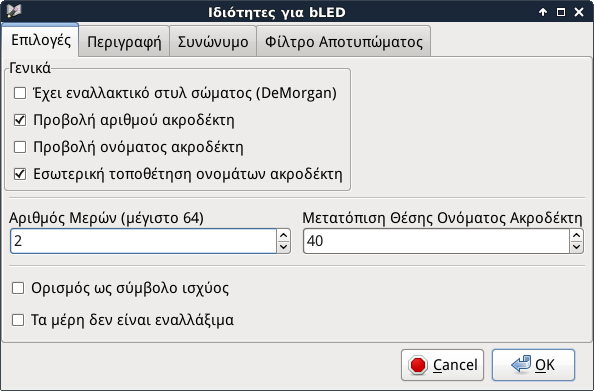
\includegraphics[width=.5\textwidth]{img/libed-dial-bledprop.png}
    \caption{Παράθυρο Ιδιοτήτων Εξαρτήματος bLED}
    \label{fig:libed-dial-bledprop}
  \end{center}
\end{figure}

Αλλάξτε τον αριθμό των μερών από 1 σε 2, και πατήστε ΟΚ για να επιστρέψετε στην κεντρική οθόνη του Επεξεργαστή Βιβλιοθήκης Εξαρτημάτων.

Πλέον το εξάρτημά μας αποτελείται από δύο μέρη. Το ποιο μέρος του εξαρτήματος (μέρος Α ή μέρος Β) επεξεργάζεστε ανά πάσα στιγμή φαίνεται στο πάνω δεξιά μέρος της κεντρικής οθόνης του Επεξεργαστή Βιβλιοθήκης Εξαρτημάτων (σχήμα \ref{fig:libed-ui-unit}).

\begin{figure}
  \begin{center}
    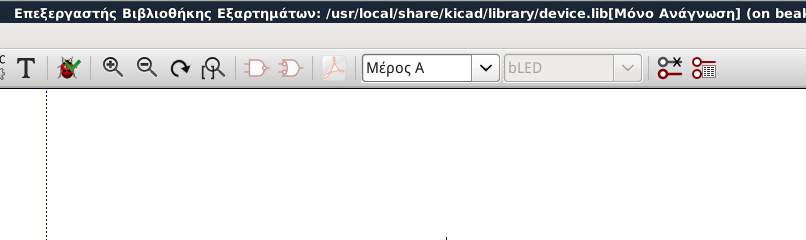
\includegraphics[width=.5\textwidth]{img/libed-ui-unit.png}
    \caption{Ένδειξη μέρους εξαρτήματος}
    \label{fig:libed-ui-unit}
  \end{center}
\end{figure}

Αφού πλέον το εξάρτημα bLED αποτελείται από δύο μέρη, πρέπει να αριθμήσουμε τους ακροδέκτες του μέρους Α ως 1 και 3 και τους ακροδέκτες του μέρους Β ως 2 και 4.

Για να το κάνουμε αυτό, επιλέγουμε στην Ένδειξη μέρους εξαρτήματος το μέρος A, και φροντίζουμε οι δύο ακροδέκτες να έχουν αριθμό 1 (άνοδος διόδου) και 3 (κάθοδος) (σχήμα \ref{fig:libed-circ-bleda}). Μπορούμε να αλλάξουμε τον αριθμό ενός ακροδέκτη κάνοντας δεξί κλικ επάνω στον ακροδέκτη και επιλέγοντας Επεξεργασία Ακροδέκτη.

Παρομοίως, επιλέγουμε στην Ένδειξη μέρους εξαρτήματος το Μέρος B, και φροντίζουμε οι δύο ακροδέκτες να έχουν αριθμό 2 (άνοδος) και 4 (κάθοδος) (σχήμα \ref{fig:libed-circ-bledb}). 

\begin{figure}
  \begin{center}
    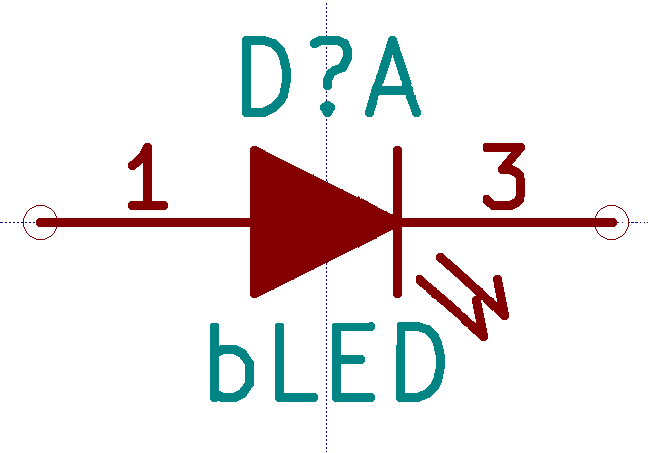
\includegraphics[width=.35\textwidth]{img/libed-circ-bleda.png}
    \caption{Εξάρτημα bLED - Μέρος Α}
    \label{fig:libed-circ-bleda}
  \end{center}
\end{figure}

\begin{figure}
  \begin{center}
    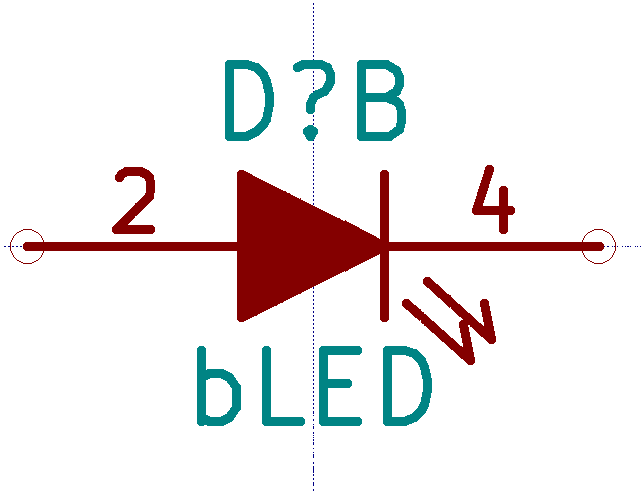
\includegraphics[width=.35\textwidth]{img/libed-circ-bledb.png}
    \caption{Εξάρτημα bLED - Μέρος Β}
    \label{fig:libed-circ-bledb}
  \end{center}
\end{figure}

Αφού έχετε ορίσει τους αριθμούς των ακροδεκτών, δεν μένει παρά να αποθηκεύσουμε το εξάρτημα.

Αποθηκεύστε την εργασία σας επιλέγοντας από το μενού στο πάνω μέρος της οθόνης \textit{Αρχείο $\rightarrow$ Αποθήκευση της τρέχουσας βιβλιοθήκης}. Θα εμφανιστούν δύο παράθυρα που θα ζητούν την επιβεβαίωση αυτή της αποθήκευσης. Επιλέξτε καταφατικά και στα δύο.

Kλείστε τον Επεξεργαστή Βιβλιοθήκης Εξαρτημάτων ώστε να επιστρέψετε στην αρχική οθόνη του \textenglish{KiCad}.

%Σε αυτό το σημείο αντιστοιχούν τα αρχεία από το αρχείο kicad\_tut03.zip.

\subsection{Σχεδίαση κυκλώματος}
Εφόσον έχουμε ετοιμάσει όλα τα εξαρτήματα που θα χρειαστούμε, πρέπει να σχεδιάσουμε το σχηματικό κύκλωμα. 

Βεβαιωθείτε ότι είστε στην αρχική οθόνη του \textenglish{KiCad} και έχετε φορτώσει το έργο usb2uart.

Από το μενού στο πάνω μέρος της οθόνης επιλέγουμε \textit{Εργαλεία $\rightarrow$ Εκτέλεση \textenglish{EEschema}}, για να εκτελεστεί η εφαρμογή \textenglish{EEschema} με την οποία σχεδιάζουμε το σχηματικό κύκλωμα. 

\subsubsection{Προσθήκη εξαρτημάτων}

Πρέπει να βρίσκεστε στην αρχική οθόνη της εφαρμογής \textenglish{EEschema}, και να είναι φορτωμένο το φύλλο του σχηματικού κυκλώματος του έργου usb2uart (σχήμα \ref{fig:eesch-circ-noic}).

\begin{figure}
  \begin{center}
    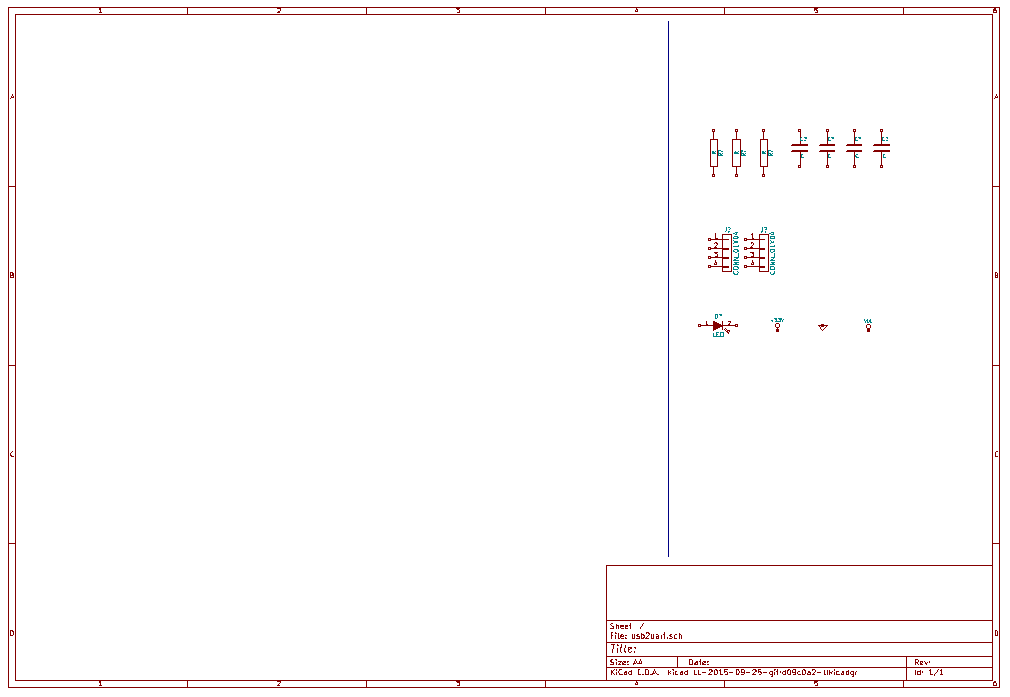
\includegraphics[width=.9\textwidth]{img/eesch-circ-noic.png}
    \caption{Το σχηματικό κύκλωμα του έργου usb2uart, έως τώρα}
    \label{fig:eesch-circ-noic}
  \end{center}
\end{figure}

Αρχικά πρέπει να προσθέσουμε στο κύκλωμα τα εξαρτήματα CP2104 και bLED. 

Όπως κάναμε και σε προηγούμενα κεφάλαια, επιλέξτε από το μενού \textit{Τοποθέτηση $\rightarrow$ Εξάρτημα}, επιλέξτε το CP2104 από τη βιβλιοθήκη usb2uart, και τοποθετήστε το στο κύκλωμα. Στη συνέχεια κάντε το ίδιο για να τοποθετήσετε το εξάρτημα bLED (και τα δύο μέρη), από την ίδια βιβλιοθήκη. Το εξάρτημα bLED αποτελείται από δύο μέρη, οπότε πρέπει να προσθέσετε πρώτα το Μέρος Α και μετά το μέρος Β.

Να σημειωθεί ότι αντί να προσθέσουμε δύο φορές το bLED (μία το Μέρος Α, και μία το Μέρος Β), θα μπορούσαμε να το προσθέσουμε μία φορά, μετά να κάναμε αντιγραφή του (δεξί κλικ στο εξάρτημα \textit{$\rightarrow$ Αντιγραφή Εξαρτήματος}), και μετά να αλλάζαμε στις ιδιότητες του αντίγραφου το Μέρος. Το αποτέλεσμα θα ήταν το ίδιο.

Πλέον πρέπει να έχουμε φορτώσει στο φύλλο όλα τα εξαρτήματα που χρειαζόμαστε για το κύκλωμά μας (σχήμα \ref{fig:eesch-circ-allcomp}).

\begin{figure}
  \begin{center}
    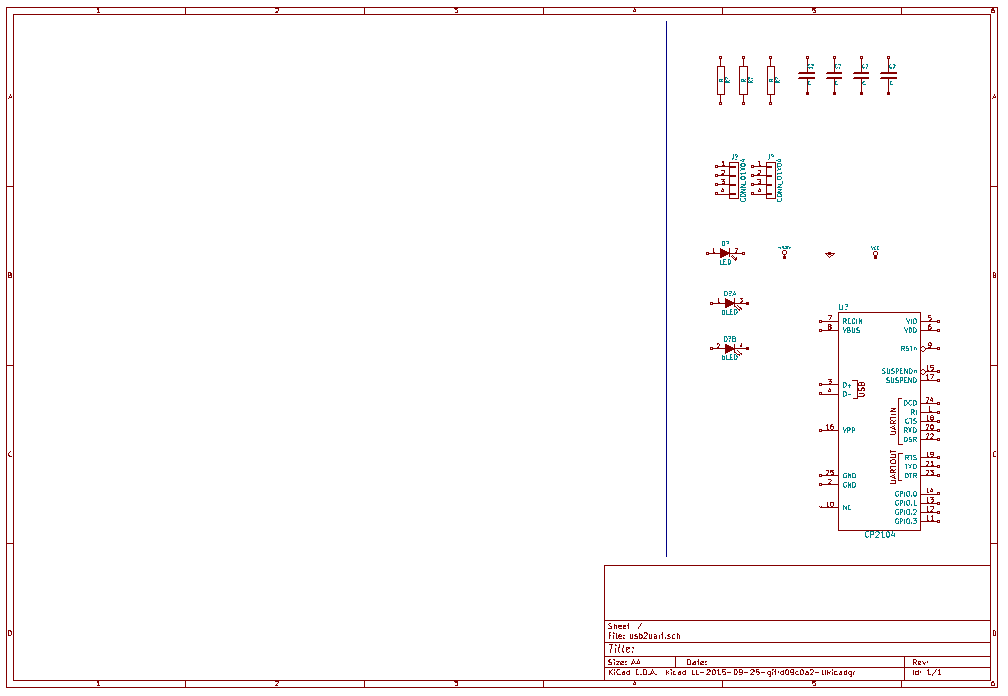
\includegraphics[width=.9\textwidth]{img/eesch-circ-allcomp.png}
    \caption{Φύλλο σχηματικού κυκλώματος έργου usb2uart με όλα τα εξαρτήματα που χρειαζόμαστε}
    \label{fig:eesch-circ-allcomp}
  \end{center}
\end{figure}

%Σε αυτό το σημείο αντιστοιχούν τα αρχεία από το αρχείο kicad\_tut04.zip.

\subsubsection{Βασικές λειτουργίες}

Πλέον αφού έχουμε όλα τα απαραίτητα εξαρτήματα στο φύλλο μας, πρέπει να τα τοποθετήσουμε στο φύλλο με τρόπο που να μας βοηθάει στην κατανόηση του κυκλώματος, και (κυρίως) να κάνουμε όλες τις συνδέσεις μεταξύ τους.

Κάποιες βασικές λειτουργίες για τη σχεδίαση του κυκλώματος είναι οι παρακάτω.

\paragraph{Μετακίνηση εξαρτήματος}
Μετατοπίζουμε το εξάρτημα όπου θέλουμε πάνω στο φύλλο του κυκλώματος. Η θέση αυτή δεν έχει κάποια ηλεκτρική σημασία, βοηθάει όμως στην καλύτερη οργάνωση του κυκλώματος. Για παράδειγμα το μοναδικό ολοκληρωμένο ενός κυκλώματος καλό θα ήταν να είναι στο μέσο του φύλλου ώστε να υπάρχει χώρος να τοποθετηθούν και άλλα εξαρτήματα γύρω του.

Για να μετακινήσουμε ένα εξάρτημα κάνουμε κλικ επάνω του, από το μενού που εμφανίζεται επιλέγουμε Μετακίνηση Εξαρτήματος, και μετά το τοποθετούμε όπου θέλουμε στο φύλλο. 

Εναλλακτικά μπορούμε να πάμε τον δείκτη του ποντικιού επάνω από το εξάρτημα (χωρίς να κάνουμε κλικ) και να πατήσουμε το πλήκτρο m.

\paragraph{Περιστροφή εξαρτήματος}
Περιστρέφουμε το εξάρτημα πάνω στο φύλλο του κυκλώματος. Η θέση περιστροφής δεν έχει κάποια ηλεκτρική σημασία, βοηθάει όμως στην καλύτερη οργάνωση του κυκλώματος. Για παράδειγμα μία αντίσταση μπορεί να προτιμάμε να εμφανίζεται οριζόντια για να διαβάζεται πιο εύκολα το όνομά της.

Για να περιστρέψουμε ένα εξάρτημα κάνουμε δεξί κλικ επάνω του, και από το μενού που εμφανίζεται επιλέγουμε \textit{Προσανατολισμός Εξαρτήματος $\rightarrow$ Περιστροφή Αριστερόστροφα (ή Περιστροφή Δεξιόστροφα)}. 

Εναλλακτικά μπορούμε να πάμε τον δείκτη του ποντικιού επάνω από το εξάρτημα (χωρίς να κάνουμε κλικ) και να πατήσουμε το πλήκτρο r.

\paragraph{Τοποθέτηση σύρματος}
Είναι από τις πιο σημαντικές λειτουργίες, καθώς με αυτή συνδέουμε αγώγιμα τα εξαρτήματα μεταξύ ενώνοντάς τα με σύρμα (σχήμα \ref{fig:eesch-circ-twoconn} και σχήμα \ref{fig:eesch-circ-twonotconn}).

Για να ενώσουμε αγώγιμα δύο σημεία του κυκλώματος (πχ τα άκρα δύο αντιστάσεων) από το μενού στο πάνω μέρος της οθόνης επιλέγουμε \textit{Τοποθέτηση $\rightarrow$ Σύρμα}, μετά κάνουμε αριστερό κλικ με το ποντίκι πάνω στο κύκλωμα μία φορά για να ξεκινήσει το σύρμα, μετά κάνουμε κλικ όσες φορές θέλουμε για να ορίσουμε τη διαδρομή, και όταν έχουμε τοποθετήσει όσο σύρμα θέλουμε κάνουμε δεξί κλικ και επιλέγουμε Τέλος Σύρματος. 

Εναλλακτικά μπορούμε να επιλέξουμε το κουμπί Τοποθέτηση σύρματος 
\includegraphics[scale=.5]{img/eesch-ico-wire.png} στη δεξιά μπάρα, και μετά να πατήσουμε το πλήκτρο w για να αρχίσουμε να τοποθετούμε σύρμα και το πλήκτρο k για ορίσουμε το τέλος του σύρματος.

\begin{figure}
  \begin{center}
    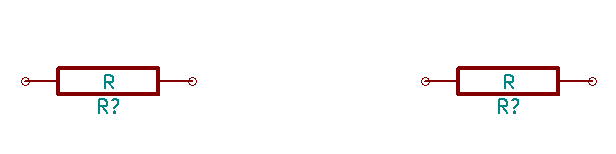
\includegraphics[width=.35\textwidth]{img/eesch-circ-twonotconn.png}
    \caption{Δυο εξαρτήματα (αντιστάσεις) χωρίς σύρμα να ενώνει τα άκρα τους}
    \label{fig:eesch-circ-twonotconn}
  \end{center}
\end{figure}

\begin{figure}
  \begin{center}
    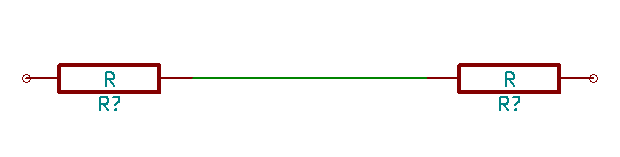
\includegraphics[width=.35\textwidth]{img/eesch-circ-twoconn.png}
    \caption{Δυο εξαρτήματα (αντιστάσεις) με σύρμα να ενώνει τα άκρα τους}
    \label{fig:eesch-circ-twoconn}
  \end{center}
\end{figure}
   
\begin{figure}
  \begin{center}
    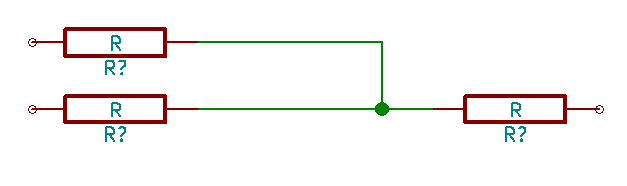
\includegraphics[width=.35\textwidth]{img/eesch-circ-threeconn.png}
    \caption{Δύο σύρματα συνδεδεμένα με τον ίδιο ακροδέκτη, με κόμβο}
    \label{fig:eesch-circ-threeconn}
  \end{center}
\end{figure}

Αξίζει να σημειωθεί ότι όταν συνδέουμε ένα σύρμα με ένα άλλο σύρμα, το \textenglish{KiCad} εμφανίζει ένα σύμβολο κόμβου 
\includegraphics[scale=.5]{img/eesch-ico-junc.png}
. Όταν θέλουμε να συνδέσουμε δύο σύρματα σε έναν ακροδέκτη (σχήμα \ref{fig:eesch-circ-threeconn}), συνήθως συνδέουμε το ένα σύρμα στον ακροδέκτη και το δεύτερο σύρμα το συνδέουμε πάνω πάνω στο πρώτο σύρμα, δημιουργώντας έναν κόμβο (σχήμα \ref{fig:eesch-circ-twowireconn}). Αν δεν δημιουργηθεί κόμβος, τα σύρματα διασταυρώνονται αλλά δεν έχουν αγώγιμη επαφή (σχήμα \ref{fig:eesch-circ-twowirenoconn}).

\begin{figure}
  \begin{center}
    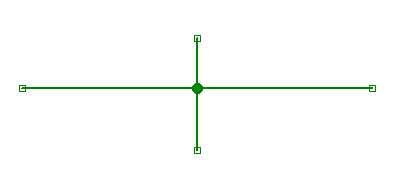
\includegraphics[width=.35\textwidth]{img/eesch-circ-twowireconn.png}
    \caption{Δύο σύρματα που έχουν αγώγιμη επαφή (κόμβο)}
    \label{fig:eesch-circ-twowireconn}
  \end{center}
\end{figure}

\begin{figure}
  \begin{center}
    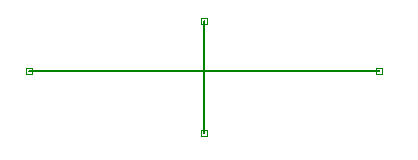
\includegraphics[width=.35\textwidth]{img/eesch-circ-twowirenoconn.png}
    \caption{Δύο σύρματα που δεν έχουν αγώγιμη επαφή (κόμβο)}
    \label{fig:eesch-circ-twowirenoconn}
  \end{center}
\end{figure}

Συνηθίζεται τα σύρματα να έχουν μόνο κατακόρυφη και οριζόντια φορά (να μην τοποθετούνται διαγώνια δύρματα), διότι έτσι παράγονται πιο ευανάγνωστα κυκλώματα.

\paragraph{Τοποθέτηση ετικέτας}
Μία ετικέτα είναι ένα αντικείμενο του κυκλώματος που συμβολίζει έναν κόμβο, ένα σημείο σύνδεσης. Αν σχεδιάσουμε πχ ένα σύρμα από το εξάρτημα Α προς μία ετικέτα Χ και μετά ένα σύρμα από το εξάρτημα Β προς τη ίδια ετικέτα Χ, τότε τα δύο εξαρτήματα θα είναι συνδεδεμένα μεταξύ τους. Η συνδεσμολογία όπου δύο εξαρτήματα είναι συνδεδεμένα μεταξύ τους απευθείας (σχήμα \ref{fig:eesch-circ-twoconnnolbl}) είναι απόλυτα ισοδύναμη με τη συνδεσμολογία όπου δύο εξαρτήματα είναι συνδεδεμένα μεταξύ τους μέσω ετικέτας (σχήμα \ref{fig:eesch-circ-twoconnlbl}).

\begin{figure}
  \begin{center}
    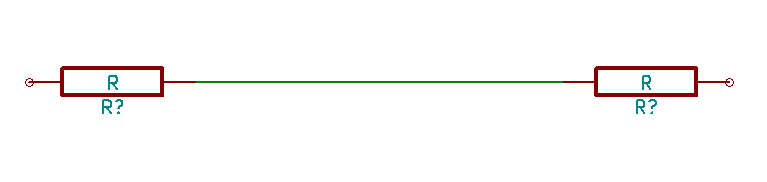
\includegraphics[width=.35\textwidth]{img/eesch-circ-twoconnnolbl.png}
    \caption{Δύο εξαρτήματα, συνδεδεμένα μεταξύ τους απευθείας}
    \label{fig:eesch-circ-twoconnlbl}
  \end{center}
\end{figure}

\begin{figure}
  \begin{center}
    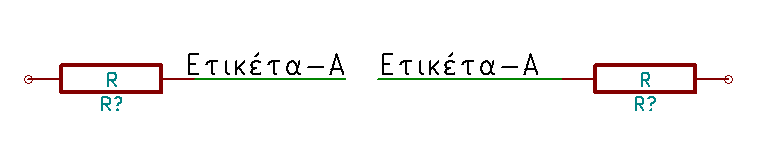
\includegraphics[width=.35\textwidth]{img/eesch-circ-twoconnlbl.png}
    \caption{Δύο εξαρτήματα, συνδεδεμένα μεταξύ τους μέσω ετικέτας}
    \label{fig:eesch-circ-twoconnnolbl}
  \end{center}
\end{figure}

Για να τοποθετήσουμε μία ετικέτα, από το μενού στο πάνω μέρος της οθόνης επιλέγουμε \textit{Τοποθέτηση $\rightarrow$ Ετικέτα}, μετά κάνουμε κλικ με το ποντίκι πάνω στο κύκλωμα, στο παράθυρο που εμφανίζεται δίνουμε ένα όνομα στην ετικέτα και πατάμε ΟΚ για να τοποθετήσουμε την ετικέτα πάνω στο κύκλωμα. 

Στη συνέχεια πρέπει να μετακινήσουμε την ετικέτα ώστε το κουτάκι που υπάρχει κάτω αριστερά από το όνομά της να συμπέσει με το κουτάκι που υπάρχει στο τέλος ενός ασύνδετου σύρματος (σχήμα \ref{fig:eesch-circ-lblok}). Εφόσον αυτά τα δύο κουτάκια είναι στο ίδιο σημείο (συμπίπτουν), τότε δεν εμφανίζονται στην οθόνη και πλέον το σύρμα έχει αυτή την ετικέτα, και θεωρείται συνδεδεμένο με όλα τα άλλα σύρματα που έχουν ετικέτα με το ίδιο όνομα. Λέμε ότι όλα αυτά τα σύρματα ανήκουν στο ίδιο δίκτυο. 

Αν τα δύο κουτάκια (του σύρματος και της ετικέτας) δεν συμπίπτουν, τότε φαίνονται και τα δύο στην οθόνη και αυτό σημαίνει ότι η ετικέτα δεν έχει τοποθετηθεί σωστά (σχήμα \ref{fig:eesch-circ-lblnotok}).

\begin{figure}
  \begin{center}
    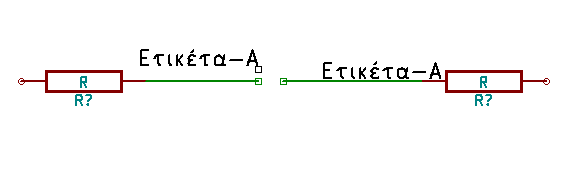
\includegraphics[width=.35\textwidth]{img/eesch-circ-lblnotok.png}
    \caption{Λάθος τοποθετημένες ετικέτες}
    \label{fig:eesch-circ-lblnotok}
  \end{center}
\end{figure}

\begin{figure}
  \begin{center}
    \includegraphics[width=.35\textwidth]{img/eesch-circ-lblok.png}
    \caption{Σωστά τοποθετημένες ετικέτες}
    \label{fig:eesch-circ-lblok}
  \end{center}
\end{figure}

\paragraph{Διαγραφή αντικειμένου}
Για να διαγράψουμε ένα αντικείμενο από το φύλλο μας (πχ ένα κομμάτι σύρματος που αποφασίσαμε να τοποθετήσουμε διαφορετικά), κάνουμε δεξί κλικ επάνω του και από το μενού που εμφανίζεται επιλέγουμε Διαγραφή.

Εναλλακτικά μπορούμε να πάμε τον δείκτη του ποντικιού επάνω από το εξάρτημα (χωρίς να κάνουμε κλικ) και να πατήσουμε το πλήκτρο Delete στο πληκτρολόγιο.

Έχοντας κατανοήσει τις παραπάνω λειτουργίες, μπορούμε να σχεδιάσουμε το κύκλωμά μας.

\subsubsection{Σχεδίαση κυκλώματος}

Για ευκολία στη σχεδίαση συνδέσεων μετακινήστε το CP2104 ώστε να είναι στο κέντρο της σελίδας.

Στη συνέχεια, μετακινήστε το VCC πάνω αριστερά από το CP2104 και συνδέστε με σύρμα τους ακροδέκτες 7 και 8 του CP2104 με το εξάρτημα VCC. Για να το κάνετε, συνδέσετε με σύρμα τον ακροδέκτη 7 με το εξάρτημα VCC και στη συνέχεια τοποθετήστε ένα σύρμα από τον  ακροδέκτη 7 προς οποιοδήποτε σημείο του προηγούμενου σύρματος (σχήμα \ref{fig:eesch-circ-78vcc}).

\begin{figure}
  \begin{center}
    \includegraphics[width=.35\textwidth]{img/eesch-circ-78vcc.png}
    \caption{Σύνδεση ακροδεκτών 7 και 8 του CP2104 με το εξάρτημα VCC}
    \label{fig:eesch-circ-78vcc}
  \end{center}
\end{figure}

Στη συνέχεια, συνδέστε με σύρμα τους ακροδέκτες 5,6 και 9 του CP2104 με το 3.3V.

Στη συνέχεια, συνδέστε με σύρμα τους ακροδέκτες 2 και 25 του CP2104 με το GND.

Για να κάνετε τα παραπάνω, ίσως χρειαστεί να μετακινήσετε τα VCC, 3.3V και GND σε πιο βολικές θέσεις στο φύλλο. Για παράδειγμα, το VCC καλό θα ήταν να τοποθετηθεί πάνω αριστερά από το CP2104 (σχήμα \ref{fig:eesch-circ-initpwrconn}).

\begin{figure}
  \begin{center}
    \includegraphics[width=.35\textwidth]{img/eesch-circ-initpwrconn.png}
    \caption{Το κύκλωμα με τις αρχικές συνδέσεις των VCC, 3.3V και GND}
    \label{fig:eesch-circ-initpwrconn}
  \end{center}
\end{figure}

Στη συνέχεια, αλλάξτε τις τιμές στους τέσσερις πυκνωτές ώστε οι τέσσερις πυκνωτές να έχουν τιμές 1u, 1u, 100n και 470n, και όχι απλά C. Οι τιμές αυτές δεν έχουν κάποια λειτουργική σημασία στο κύκλωμα, αλλά βοηθούν στην οργάνωση των εξαρτημάτων. Για να αλλάξετε τις τιμές κάντε δεξί κλικ πάνω στον πυκνωτή και επιλέξετε \textit{Επεξεργασία Εξαρτήματος $\rightarrow$ Τιμή}.

Στη συνέχεια, συνδέστε τους πυκνωτές 1u και 100n ως bypass στο 3.3V, δηλαδή ανάμεσα στο 3.3v και στο GND. 

Για να το κάνετε αυτό και το κύκλωμα να παραμείνει ευανάγνωστο μπορείτε να προσθέσετε επιπλέον εξαρτήματα GND. Όλα τα εξαρτήματα GND που θα προσθέσετε συμβολίζουν το ίδιο σημείο, τον ίδιο κόμβο στο κύκλωμά σας, τον κόμβο της γείωσης. Ομοίως και για το +3.3V: μπορείτε να προσθέσετε επιπλέον εξαρτήματα +3.3V ώστε να είναι πιο ευανάγνωστο το κύκλωμα, και όλα τα εξαρτήματα +3.3V που θα προσθέσετε συμβολίζουν το ίδιο σημείο, τον ίδιο κόμβο στο κύκλωμά σας.

Οπότε, για τον πυκνωτή 1u προσθέστε ένα εξάρτημα GND στο φύλλο (επιλέγοντας στο μενού \textit{Τοποθέτηση $\rightarrow$ Εξάρτημα}) λίγο πιο δεξιά από το 3.3V, και μετά τοποθετήστε σύρμα που να συνδέει το 3.3V με το 1u και μετά σύρμα που να συνδέει το 1u με το (νέο) GND. Ομοίως θα κάνετε και για το 100n.

Στη συνέχεια, συνδέστε με τον ίδιο τρόπο όπως παραπάνω τον πυκνωτή 1u ως bypass στο VCC, δηλαδή συνδέστε τον ανάμεσα στο VCC και σε ένα GND.

Στη συνέχεια, συνδέστε τον πυκνωτή 470n ανάμεσα στους ακροδέκτες 16 και 2 του CP2104.

Στη συνέχεια, αλλάξτε τις τιμές στα δύο εξαρτήματα CONN\_01X04 ώστε το ένα να λέγεται USB, και το άλλο Header. Τοποθετήστε το USB αριστερά του CP2104 και το Header δεξιά του CP2104 (σχήμα \ref{fig:eesch-circ-allpwr}).

\begin{figure}
  \begin{center}
    \includegraphics[width=.9\textwidth]{img/eesch-circ-allpwr.png}
    \caption{Το κύκλωμα με τις πλήρεις συνδέσεις των VCC, 3.3V, GND και απλά τοποθετημένα τα USB, Header}
    \label{fig:eesch-circ-allpwr}
  \end{center}
\end{figure}

Στη συνέχεια, θα πρέπει να συνδέσουμε όλους τους ακροδέκτες των USB και Header. Αν συνδέαμε απευθείας μεταξύ τους όλους του ακροδέκτες το κύκλωμα δεν θα ήταν ιδιαίτερα ευανάγνωστο και οργανωμένο διότι θα υπήρχαν πολλά διασταυρούμενα (αλλά μη συνδεδεμένα) σύρματα. Για να λύσουμε αυτό το πρόβλημα, θα χρησιμοποιήσουμε ετικέτες.

Με δεδομένο το εργαλείο της ετικέτας, θα τοποθετήσουμε σύρματα ώστε να συνδέσουμε όπως θέλουμε τους ακροδέκτες των USB και Header.

Τοποθετήστε σύρμα από τον ακροδέκτη 1 του USB έως ένα VCC.

Τοποθετήστε σύρμα από τον ακροδέκτη 4 του USB έως ένα GND.

Τοποθετήστε σύρμα από τον ακροδέκτη 1 του HEADER έως ένα 3.3V.

Τοποθετήστε σύρμα από τον ακροδέκτη 4 του HEADER έως ένα GND.

Τοποθετήστε σύρμα από τον ακροδέκτη 2 του USB έως το D- του CP2104, χρησιμοποιώντας ετικέτα με όνομα USBDM.

Τοποθετήστε σύρμα από τον ακροδέκτη 3 του USB έως το D+ του CP2104, χρησιμοποιώντας ετικέτα με όνομα USBDP.

Τοποθετήστε σύρμα από τον ακροδέκτη 2 του HEADER έως το TXD του CP2104, χρησιμοποιώντας ετικέτα με όνομα TXD.

Τοποθετήστε σύρμα από τον ακροδέκτη 3 του HEADER έως το RXD του CP2104, χρησιμοποιώντας ετικέτα με όνομα RXD.

Πλέον το κύκλωμά μας έχει και όλες τις συνδέσεις των USB και Header (σχήμα \ref{fig:eesch-circ-allpwrheaders}).

\begin{figure}
  \begin{center}
    \includegraphics[width=.9\textwidth]{img/eesch-circ-allpwrheaders.png}
    \caption{Το κύκλωμα με τις πλήρεις συνδέσεις των VCC, 3.3V, GND και συνδεδεμένα τα USB, Header}
    \label{fig:eesch-circ-allpwrheaders}
  \end{center}
\end{figure}

Τώρα πρέπει να συνδέσουμε τα LED. 

Μετακινήστε τα LED (το ένα μονό και το ένα που αποτελείται από δύο μέρη) και τις τρεις αντιστάσεις στην περιοχή πάνω από το CP2104.

Στη συνέχεια, αλλάξτε τις τιμές στις τρεις αντιστάσεις του κυκλώματος ώστε να έχουν τις τιμές 220R, 220R και 430R.

Στη συνέχεια, τοποθετήστε σύρμα που να συνδέει ένα VCC με τον ένα ακροδέκτη της 430R, και τον άλλο ακροδέκτη της 430R με την κάθοδο του μονού LED και μετά την άνοδο του μονού LED με ένα GND.

Στη συνέχεια, τοποθετήστε σύρμα που να συνδέει ένα 3.3V με τον ένα ακροδέκτη της 220R, και τον άλλο ακροδέκτη της 220R με την άνοδο του bLED (Μέρος Α) και την κάθοδο του bLED (Μέρος Α), μέσω ετικέτας LEDRX, με τον ακροδέκτη 13 του CP2104.

Στη συνέχεια, τοποθετήστε σύρμα που να συνδέει ένα 3.3V με τον ένα ακροδέκτη της δεύτερης 220R, και τον άλλο ακροδέκτη της δεύτερης 220R με την άνοδο του bLED (Μέρος Β) και την κάθοδο του bLED (Μέρος Β), μέσω ετικέτας LEDΤX, με τον ακροδέκτη 14 του CP2104.

Στη συνέχεια, προσθέστε κείμενο δίπλα στα LED ώστε να είναι σαφές τι χρώμα είναι το κάθε ένα (μονό LED = μπλε, A = πράσινο, B = πορτοκαλί). Για να προσθέσουμε κείμενο, επιλέγουμε από τη δεξιά μπάρα το το εικονίδιο \textit{Τοποθέτηση κειμένου} \includegraphics[scale=.5]{img/eesch-ico-text.png}, κάνουμε κλικ στο φύλλο, και στο παράθυρο που εμφανίζεται γράφουμε ό,τι κείμενο θέλουμε, επιλέγουμε αν θα εμφανίζεται κάθετα, τι στοίχιση θα έχει, κοκ.

Πλέον έχουμε ολοκληρώσει τη συνδεσμολογία των LED (σχήμα \label{fig:eesch-circ-ledonly}).

\begin{figure}
  \begin{center}
    \includegraphics[width=.9\textwidth]{img/eesch-circ-ledonly.png}
    \caption{Συνδεσμολογία LED (δεν φαίνονται οι αντίστοιχες ετικέτες LEDTX, LEDRX του CP2104)}
    \label{fig:eesch-circ-ledonly}
  \end{center}
\end{figure}

Τέλος, για λόγους καλύτερης οργάνωσης, πρέπει να προσθέσουμε ετικέτες και στα υπόλοιπα δίκτυα του κυκλώματός μας, και συγκεκριμένα στο VPP (ετικέτα VPP), και στα σύρματα ανάμεσα στις αντιστάσεις και τα LED (ετικέτες LEDONR, LEDRXR και LEDTXR).

Πλέον έχουμε σχεδιάσει πλήρως το κύκλωμα. Για λόγους καλύτερης οργάνωσης, και ηλεκτρολογικού ελέγχου του κυκλώματος, χρειαζόμαστε ακόμα δύο βήματα.

Καταρχάς πρέπει σε όλους τους ακροδέκτες που δεν έχουν κάτι συνδεδεμένο επάνω τους (όπως πχ οι ακροδέκτες 15 και 17 του CP2104) να τοποθετήσουμε ένα σύμβολο Μη Σύνδεσης. Αυτό θα βοηθήσει στο να δηλώσουμε στο \textenglish{KiCad} ότι ο συγκεκριμένος ακροδέκτης θέλουμε όντως να μην συνδέεται πουθενά και δεν έχουμε απλά ξεχάσει να τον συνδέσουμε. Για να τοποθετήσουμε σύμβολο Μη Σύνδεσης, επιλέγουμε από το μενού στο πάνω μέρος της οθόνης \textit{Τοποθέτηση $\rightarrow$ Σήμανση Μη Σύνδεσης} και κάνουμε κλικ στο σημείο όπου θέλουμε να το τοποθετήσουμε. Πρέπει να τοποθετήσουμε μία Σήμανση Μη Σύνδεσης σε κάθε ακροδέκτη του CP2104 που δεν συνδέεται με κάτι άλλο.

Κατά δεύτερον, πρέπει στα δίκτυα VCC και GND να συνδέσουμε μέσω σύρματος από ένα εξάρτημα PWR\_FLAG (από τη βιβλιοθήκη power). Με αυτό τον τρόπο το \textenglish{KiCad}, όταν κάνει ηλεκτρολογικό έλεγχο, θα καταλάβει ότι τα δύο δίκτυα αυτά είναι δίκτυα ισχύος, και ότι υπάρχει ισχύς στο κύκλωμά μας.

Πλέον έχουμε ολοκληρώσει πλήρως το σχηματικό κύκλωμα (σχήμα \ref{fig:eesch-schem-final2}).

\begin{figure}
  \begin{center}
    \includegraphics[width=.9\textwidth]{img/eesch-schem-final.png}
    \caption{Πλήρως σχεδιασμένο κύκλωμα}
    \label{fig:eesch-schem-final2}
  \end{center}
\end{figure}

\subsubsection{Ονοματοδοσία κυκλώματος}
Αφού έχουμε ολοκληρώσει τον σχεδιασμό του κυκλώματος, πρέπει να δώσουμε ονομασίες αναφοράς σε όλα τα εξαρτήματα, ώστε οι αντιστάσεις να έχουν ονομασία αναφοράς R1, R2, R3 κοκ. Να σημειωθεί ότι η ονομασία αναφοράς είναι διαφορετική έννοια από την τιμή (πχ 220R). 

Ονομασίες αναφοράς μπορούμε να δώσουμε μόνοι μας, κάνοντας επεξεργασία σε κάθε ένα εξάρτημα ή μπορούμε να πούμε στο \textenglish{KiCad} να δώσει αυτόματα ονομασίες αναφοράς σε όλα τα εξαρτήματα. Για να το το κάνουμε αυτό, επιλέγουμε από το μενού στο πάνω μέρος της οθόνης \textit{Εργαλεία $\rightarrow$ Ονοματοδοσία σχηματικού}, στο παράθυρο που εμφανίζεται δεν αλλάζουμε καμία ρύθμιση και κάνουμε κλικ στο Ονοματοδοσία.

\begin{figure}
  \begin{center}
    \includegraphics[width=.5\textwidth]{img/eesch-dial-annot.png}
    \caption{Παράθυρο Ονοματοδοσίας}
    \label{fig:eesch-dial-annot}
  \end{center}
\end{figure}

Όταν ολοκληρωθεί η διαδικασία, όλα τα εξαρτήματα θα έχουν συγκεκριμένες, αριθμημένες ονομασίες αναφοράς (και όχι ερωτηματικά).


\subsubsection{Έλεγχος Ηλεκτρικών Κανόνων}
Αφού ολοκληρωθεί η ονοματοδοσία, πρέπει να κάνουμε Έλεγχο Ηλεκτρικών Κανόνων στο κύκλωμα, ώστε το \textenglish{KiCad} να αναλύσει το κύκλωμα και να μας ενημερώσει για πιθανά προβλήματα όπως πχ αν έχουμε ξεχάσει να συνδέσουμε ένα δίκτυο ή αν ένας ακροδέκτης εξαρτήματος έχει χαρακτηρισμό Είσοδος αλλά είναι συνδεδεμένος με έναν ακροδέκτη που έχει επίσης χαρακτηρισμό Είσοδος.

Για να κάνουμε Έλεγχο Ηλεκτρικών Κανόνων, επιλέγουμε από το μενού στο πάνω μέρος της οθόνης \textit{Εργαλεία $\rightarrow$ Ελεγκτής Ηλεκτρικών Κανόνων} και στο παράθυρο που εμφανίζεται δεν αλλάζουμε καμία ρύθμιση και κάνουμε κλικ στο Εκτέλεση. 

Αν έχετε χρησιμοποιήσει τα αρχεία του tutorial, ο Ελεγκτής Ηλεκτρικών Κανόνων πρέπει να σας βγάλει μία προειδοποίηση: ότι ο ακροδέκτης 9 (χαρακτηρισμένος ως αμφίδρομος στο εξάρτημα) του CP2104 είναι συνδεδεμένος με τον ακροδέκτη 6 (χαρακτηρισμένος ως έξοδος) του CP2104. Αυτό φαίνεται στο \textenglish{KiCad} να είναι λάθος διότι ένας ακροδέκτης έξοδος πρέπει να είναι συνδεδεμένος με έναν ακροδέκτη είσοδο και όχι έναν αμφίδρομο. Στη συγκεκριμένη περίπτωση πρόκειται για απλό θέμα χαρακτηρισμού του ακροδέκτη 9 και μπορούμε να αγνοήσουμε την προειδοποίηση. Οπότε απλά κλείστε το παράθυρο του Ελεγκτή.
Εναλλακτικά, μπορούμε να επεξεργαστούμε το εξάρτημα CP2104 με το σχετικό εργαλείο και να αλλάξουμε τον χαρακτηρισμό του ακροδέκτη 9 σε είσοδο.

\subsubsection{Εκτύπωση σχηματικού σε pdf}
Τέλος, αφού έχουμε ολοκληρώσει το κύκλωμά μας, καλό είναι να το κρατήσουμε και σε ένα αρχείο pdf, ώστε να είναι εύκολη η αναφορά σε αυτό χωρίς να ανοίγουμε το \textenglish{KiCad}. Για να το κάνουμε αυτό, επιλέγουμε από το μενού στο πάνω μέρος της οθόνης \textit{Αρχείο $\rightarrow$ Σχεδιογράφηση $\rightarrow$ Σχεδιογράφηση} και στο παράθυρο που εμφανίζεται επιλέγουμε Μορφή PDF, και πατάμε το κουμπί Σχεδιογράφηση Τρέχουσας Σελίδας (σχήμα \ref{fig:eesch-dial-plot}). 

\begin{figure}
  \begin{center}
    \includegraphics[width=.5\textwidth]{img/eesch-dial-plot.png}
    \caption{Παράθυρο Σχεδιογράφησης}
    \label{fig:eesch-dial-plot}
  \end{center}
\end{figure}

Πλέον το κύκλωμα υπάρχει και σε μορφή pdf, στο φάκελο όπου έχουμε και όλα τα άλλα αρχεία του έργου μας. 

\subsubsection{Δημιουργία προτύπων πεδίων για εξαρτήματα}
Έχοντας υπόψιν το ότι για αυτό το σχηματικό θα σχεδιαστεί πλακέτα η οποία θα κατασκευαστεί, θα ήταν καλό για κάθε εξάρτημα που χρησιμοποιούμε, να ξέρουμε ποιο πραγματικό εξάρτημα/υλικό θέλουμε να τοποθετηθεί στην πλακέτα. 

Για παράδειγμα, υπάρχει στο σχηματικό μία αντίσταση R1 η οποία θέλουμε να είναι 430 Ohm. Υπάρχουν όμως πολλές εταιρείες που κατασκευάζουν αντιστάσεις 430 Ohm και μάλιστα κάθε εταιρεία έχει πολλά μοντέλα για αντιστάσεις 430 Ohm. Εμείς πρέπει να κάνουμε έρευνα αγοράς και να καταλήξουμε ότι πχ θέλουμε να χρησιμοποιήσουμε την αντίσταση με κωδικό ERJ-2GEJ431X από τον κατασκευαστή Panasonic. Καλό θα ήταν αυτό να το καταγράφαμε κάπως στο σχηματικό. 

Για να το κάνουμε αυτό, θα δημιουργήσουμε νέα πεδία που θα ονομάζονται MFG (για τον κατασκευαστή) και MFG Code (για τον κωδικό εξαρτήματος) και θα ορίσουμε στο KiCad αυτά τα πεδία να υπάρχουν σε όλα τα εξαρτήματα. Οπότε θα μπορούμε σε κάθε εξάρτημα να καταγράφουμε και ποιο πραγματικό υλικό θέλουμε να χρησιμοποιηθεί κατά την κατασκευή της πλακέτας.

Για να δημιουργήσουμε νέα πεδία, επιλέγουμε από το μενού στο πάνω μέρος της οθόνης \textit{Προτιμήσεις $\rightarrow$ Επιλογές Επεξεργαστή Σχηματικού} και στο παράθυρο που εμφανίζεται, στην καρτέλα Πρότυπα Ονομάτων Πεδίων προσθέτουμε δύο πεδία. Ένα με όνομα MFG και ένα με όνομα MCF code.

Πλέον όλα τα εξαρτήματα, στις ιδιότητές τους, εκτός από Ονομασία Αναφοράς κλπ θα έχουν και πεδία όπου μπορείτε να καταχωρήσετε κατασκευαστή και κωδικό εξαρτήματος. 

Συνίσταται να πάρετε τις πληροφορίες αυτές (κατασκευαστή και κωδικό εξαρτήματος για όλα τα εξαρτήματα) από τα αρχεία του tutorial, καθώς η έρευνα αγοράς για υλικά και η εμπορική τους σύγκριση είναι μία επίπονη διαδικασία που ξεφεύγει από τα πλαίσια του tutorial. 

\begin{figure}
  \begin{center}
    \includegraphics[width=.35\textwidth]{img/eesch-dial-templ.png}
    \caption{Παράθυρο Επιλογές Επεξεργαστή Σχηματικού}
    \label{fig:eesch-dial-templ}
  \end{center}
\end{figure}

%Σε αυτό το σημείο αντιστοιχούν τα αρχεία από το αρχείο kicad\_tut05.zip.

\subsubsection{Δημιουργία Λίστας Υλικών και Λίστας Δικτύων}
Αφού έχουμε ολοκληρώσει το σχηματικό κύκλωμα, θα χρειαστεί να κρατήσουμε κάποια από τα δεδομένα του, τα οποία θα μας χρειαστούν κατά τη σχεδίαση της πλακέτας. Αυτά τα δεδομένα είναι η λίστα υλικών και η λίστα δικτύων.

Για να κρατήσουμε λίστα με όλα τα υλικά και εξαρτήματα του κυκλώματος, από το μενού επιλέγουμε \textit{Εργαλεία $\rightarrow$ Δημιουργία Λίστας Υλικών}, στο παράθυρο που εμφανίζεται επιλέγουμε Δημιουργία, και τέλος επιλέγουμε Κλείσιμο. Πλέον έχει δημιουργηθεί ένα αρχείο usb2uart.xml, στο φάκελο όπου έχουμε και όλα τα άλλα αρχεία του έργου μας. Αυτό το αρχείο είναι η λίστα υλικών (Bill Of Materials - BOM) του κυκλώματός μας, σε μορφή xml. Αυτή η μορφή μπορεί να προσαρμοστεί προγραμματιστικά σε όποια άλλη μορφή χρειαστεί. To KiCad προσφέρει κάποια πρόσθετα τα οποία μπορούν να μετατρέψουν αυτό το .xml σε κάποια πιο διαδεδομένη μορφή (όπως .csv), αλλά η χρήση τους ξεφεύγει από τα πλαίσια αυτού του tutorial.

Για να κρατήσουμε λίστα με όλα τα δίκτυα του κυκλώματος (Λίστα Δικτύων), από το μενού επιλέγουμε \textit{Εργαλεία $\rightarrow$ Δημιουργία Αρχείου Λίστας Δικτύων}, στο παράθυρο που εμφανίζεται επιλέγουμε Δημιουργία, και τέλος αποθηκεύουμε το αρχείο με όνομα usb2uart.net στο φάκελο που θέλουμε. Συνίσταται να αποθηκευτεί μαζί με όλα τα άλλα αρχεία του έργου.

%Σε αυτό το σημείο αντιστοιχούν τα αρχεία από το αρχείο kicad\_tut06.zip.

\newpage
\section{Δημιουργία Πλακέτας (PCB)}
Αφού ολοκληρώσαμε το σχηματικό κύκλωμα το επόμενο βήμα είναι να σχεδιάσουμε την πλακέτα (PCB) του κυκλώματος. Αυτό γίνεται με την εφαρμογή Pcbnew.

\subsection{Pcbnew}
Από την κεντρική οθόνη του \textenglish{KiCad} εκτελέστε την εφαρμογή Pcbnew, με την οποία θα σχεδιάσουμε την πλακέτα.

\begin{figure}
  \begin{center}
    \includegraphics[width=.9\textwidth]{img/pcb-wind-main.png}
    \caption{Κεντρική οθόνη του Pcbnew}
    \label{fig:pcb-wind-main}
  \end{center}
\end{figure}

H κεντρική οθόνη του Pcbnew αποτελείται από τα παρακάτω
\begin{itemize}
    \item ένας κενός χώρος για σχεδίαση της πλακέτας στο κέντρο της οθόνης
    \item γραμμή μενού στο πάνω μέρος της οθόνης, με όλες σχεδόν τις δυνατές λειτουργίες
    \item μπάρα βασικών λειτουργιών στο πάνω μέρος της οθόνης
    \item μπάρα με γενικές λειτουργίες στο αριστερό μέρος της οθόνης, όπως εμφάνιση περιγραμμάτων ή πλήρους σχεδιασμού, εμφάνιση ή όχι του πλέγματος, εμφάνιση ή όχι της φωλιάς συνδέσεων, κα
    \item μπάρες με συγκεκριμένες λειτουργίες σχεδίασης στο δεξί μέρος της οθόνης, όπως τοποθέτηση δρόμων, ζωνών, γραφικών σχεδίων, κα
    \item λίστα όλα τα επίπεδα της πλακέτας στο δεξί μέρος της οθόνης, όπου επιλέγουμε ποιο επίπεδο είναι ενεργό, δηλαδή σε ποιο επίπεδο σχεδιάζουμε
    \item μπάρα κατάστασης στο κάτω μέρος της οθόνης με πληροφορίες συντεταγμένων, ενεργού εξαρτήματος, κα
\end{itemize}

Καθόλη τη διάρκεια του σχεδιασμού της πλακέτας, φροντίστε να μην είναι επιλεγμένη η εμφάνιση πολικών συντεταγμένων, από την μπάρα στο αριστερό μέρος της οθόνης \includegraphics[scale=.5]{img/pcb-ico-coord.png}.


\subsection{Ρυθμίσεις σελίδας}
Αρχικά πρέπει να ορίσουμε τις ιδιότητες της σελίδας μας, από το μενού \textit{Αρχείο $\rightarrow$ Ρυθμίσεις σελίδας} (σχήμα \ref{fig:pcb-dial-pageset}). Σε αυτό το παράθυρο, ορίστε τις ρυθμίσεις της σελίδας σας, όπως μέγεθος χαρτιού, ημερομηνία έκδοσης, τίτλος κυκλώματος, και πατήστε ΟΚ. Αυτές οι ρυθμίσεις δεν έχουν κάποια ηλεκτρική ή λειτουργική σημασία για το κύκλωμα, είναι όμως χρήσιμες πληροφορίες για την οργάνωση των κυκλωμάτων σας.

\begin{figure}
  \begin{center}
    \includegraphics[width=.5\textwidth]{img/pcb-dial-pageset.png}
    \caption{Ρυθμίσεις Σελίδας Pcbnew}
    \label{fig:pcb-dial-pageset}
  \end{center}
\end{figure}

\subsection{Ορισμός επιπέδων}
Στη συνέχεια θα πρέπει να ορίσουμε τα επίπεδα από τα οποία θα αποτελείται η πλακέτα μας. Έχουμε πάρει την απόφαση ότι το κύκλωμα που θα σχεδιάσουμε θέλουμε να έχει δύο επίπεδα, και θα τοποθετηθούν εξαρτήματα μόνο στο ένα επίπεδο, το μπροστινό επίπεδο. 

Από το μενού επιλέξτε \textit{Κανόνες Σχεδίασης $\rightarrow$ Ρύθμιση Επιπέδων} (σχήμα \ref{fig:pcb-dial-layers}). Στο παράθυρο που θα εμφανιστεί επιλέξτε από πάνω αριστερά την προκαθορισμένη ομαδοποίηση "Δύο επίπεδα, εξαρτήματα μόνο Μπροστά" και φροντίστε να είναι επιλεγμένα μόνο τα παρακάτω επίπεδα
\begin{itemize}
    \item F.Paste, διότι θα έχουμε εξαρτήματα SMD στην μπροστινή πλευρά
    \item F.SilkS, διότι θα έχουμε σχέδια και κείμενα στην μπροστινή πλευρά
    \item F.Mask, διότι θα έχουμε εξαρτήματα στην μπροστινή πλευρά
    \item F.Cu, διότι θα έχουμε αγώγιμους δρόμους στην μπροστινή πλευρά
    \item B.Cu, διότι θα έχουμε αγώγιμους δρόμους στην πίσω πλευρά
    \item B.Mask, διότι θα έχουμε (μόνο διαμπερή) εξαρτήματα στην πίσω πλευρά
    \item Edge.Cuts, για να σχεδιάσουμε τα όρια της πλακέτας
    \item Dwgs.User για να μπορούμε να σχεδιάζουμε σημειώσεις, να γράφουμε μηχανικές διαστάσεις, κα
\end{itemize}

Αφού κάνετε τα παραπάνω, επιλέξτε ΟΚ και θα επανέλθετε στην κεντρική οθόνη του Pcbnew.

\begin{figure}
  \begin{center}
    \includegraphics[width=.9\textwidth]{img/pcb-dial-layers.png}
    \caption{Παράθυρο Ρύθμισης Επιπέδων}
    \label{fig:pcb-dial-layers}
  \end{center}
\end{figure}

Στο δεξί μέρος της κεντρικής οθόνης του Pcbnew υπάρχει λίστα με όλα τα επίπεδα της πλακέτας. Κάνοντας κλικ στο μικρό κουτάκι με το χρώμα αριστερά από το όνομα κάθε επιπέδου, μπορούμε να αλλάξουμε εάν θέλουμε το χρώμα που χρησιμοποιεί το \textenglish{KiCad} για να εμφανίσει κάθε επίπεδο. Συνήθως επιλέγουμε να εμφανίζεται κόκκινο το μπροστά επίπεδο χαλκού (F.Cu) και να εμφανίζεται πράσινο το πίσω επίπεδο χαλκού (B.Cu).

Επίσης σε αυτή τη λίστα φαίνεται ένα μικρό βέλος δίπλα στο επίπεδο το οποίο είναι τρέχων, το επίπεδο δηλαδή στο οποίο σχεδιάζουμε. Σε κάθε σημείο όπου σχεδιάζουμε ή τοποθετούμε κάτι στην πλακέτα μας, πρέπει να φροντίζουμε αυτό να γίνεται στο σωστό επίπεδο.

\subsection{Κανόνες σχεδίασης}
Αφού ορίσουμε τα επίπεδα, πρέπει να καθορίσουμε τους κανόνες σχεδίασης που θα διέπουν την πλακέτα μας. Αυτό περιλαμβάνει το ελάχιστο τυπικό διάκενο ανάμεσα σε δύο δρόμους, το τυπικό πλάτος δρόμου, την τυπική διάμετρο των τρυπών via, κα. Αυτές οι πληροφορίες οργανώνονται σε κλάσεις δικτύου. Μία κλάση δικτύου, δηλαδή, περιλαμβάνει πλάτος δρόμου, την διάμετρο των τρυπών via, κα. 

Από το μενού επιλέξτε \textit{Κανόνες Σχεδίασης $\rightarrow$ Κανόνες Σχεδίασης} (σχήμα \ref{fig:pcb-dial-desset}). 

Στο παράθυρο που θα εμφανιστεί ορίστε το Διάκενο στα 0,2mm το Πλάτος Δρόμου στα 0.25mm, τη Διάμετρο Via στα 0,7mm και τη Διάτρηση Via στα 0,4mm. Αφού ορίσετε αυτές τις διαστάσεις, πατήστε ΟΚ και θα επανέλθετε στην κεντρική οθόνη του Pcbnew.

\begin{figure}
  \begin{center}
    \includegraphics[width=.9\textwidth]{img/pcb-dial-desset.png}
    \caption{Παράθυρο Κανόνων Σχεδίασης}
    \label{fig:pcb-dial-desset}
  \end{center}
\end{figure}

Επίσης πρέπει να οριστούν κάποια βασικά μεγέθη για τις έδρες των αποτυπωμάτων. Από το μενού επιλέξτε \textit{Διαστάσεις $\rightarrow$ Διάκενο Μάσκας Εδρών} και στο παράθυρο που εμφανίζεται ορίστε τις παρακάτω ρυθμίσεις (σχήμα \ref{fig:pcb-dial-padclear}).

\begin{itemize}
    \item Διάκενο μάσκας συγκόλλησης +0,05mm
    \item Ελάχιστο πλάτος μάσκας συγκόλησης 0,25mm
    \item Διάκενο πάστας συγκόλησης -0,02mm
\end{itemize}

\begin{figure}
  \begin{center}
    \includegraphics[width=.5\textwidth]{img/pcb-dial-padclear.png}
    \caption{Παράθυρο Διάκενου Μάσκας Εδρών}
    \label{fig:pcb-dial-padclear}
  \end{center}
\end{figure}

Πλέον έχουμε ορίσει τα βασικά ηλεκτρικά χαρακτηριστικά της πλακέτας μας.
%Σε αυτό το σημείο αντιστοιχούν τα αρχεία από το αρχείο kicad\_tut07.zip.

\subsection{Ορισμός βιβλιοθηκών έργου}
Στη συνέχεια θα χρειαστεί να ορίσουμε τις βιβλιοθήκες αποτυπωμάτων που θα χρησιμοποιήσουμε. Αξίζει να σημειωθεί ότι ο τρόπος που προσθέτουμε βιβλιοθήκες αποτυπωμάτων είναι αρκετά διαφορετικός από τον τρόπο προσθήκης βιβλιοθήκης εξαρτημάτων. Επίσης τρόπος που προσθέτουμε βιβλιοθήκες αποτυπωμάτων στην τρέχουσα έκδοση του KiCad διαφέρει αρκετά από τις προηγούμενες εκδόσεις, καθώς πλέον χρησιμοποιείται και ένα αρχείο με όνομα fp-lib-table (κατάλογος βιβλιοθήκης), ενώ οι περισσότερες βιβλιοθήκες είναι σε διαδικτυακά αποθετήρια και δεν περιλαμβάνονται στη διανομή του KiCad.

Από το μενού επιλέξτε \textit{Προτιμήσεις $\rightarrow$ Διαχειριστής Βιβλιοθηκών Αποτυπωμάτων}. Σε αυτό το παράθυρο (σχήμα \ref{fig:pcb-dial-libs}), επιλέξτε Προσθήκη με Οδηγό (σχήμα \ref{fig:pcb-dial-libwiz}) και ακολουθήστε τα βήματα που προτείνει ο οδηγός ώστε προσθέσετε από το αποθετήριο https://github.com/KiCad τις παρακάτω βιβλιοθήκες στο έργο σας, και αυτές να αποθηκευτούν τοπικά στον υπολογιστή σας, μαζί με τα άλλα αρχεία του έργου σας. Για να ολοκληρωθεί αυτή η διαδικασία, ο υπολογιστής σας πρέπει να έχει ενεργή πρόσβαση στο διαδίκτυο (σχήματα \ref{fig:pcb-dial-libwiz}, \ref{fig:pcb-dial-libwiz2} και \ref{fig:pcb-dial-libwiz3})

\begin{itemize}
    \item LEDs.pretty
    \item Capacitors\_SMD.pretty
    \item Resistors\_SMD.pretty
    \item SMD\_Packages.pretty
    \item Pin\_Headers.pretty
    \item Connect.pretty
\end{itemize}

Οι βιβλιοθήκες πρέπει να προστεθούν μόνο στο τρέχον Έργο και όχι ως Καθολικές.

\begin{figure}
  \begin{center}
    \includegraphics[width=.9\textwidth]{img/pcb-dial-libs.png}
    \caption{Παράθυρο Διαχειριστή Βιβλιοθηκών Αποτυπωμάτων}
    \label{fig:pcb-dial-libs}
  \end{center}
\end{figure}

\begin{figure}
  \begin{center}
    \includegraphics[width=.9\textwidth]{img/pcb-dial-libwiz.png}
    \caption{Οδηγός Προσθήκης Βιβλιοθηκών Αποτυπωμάτων - Έναρξη}
    \label{fig:pcb-dial-libwiz}
  \end{center}
\end{figure}

\begin{figure}
  \begin{center}
    \includegraphics[width=.9\textwidth]{img/pcb-dial-libwiz2.png}
    \caption{Οδηγός Προσθήκης Βιβλιοθηκών Αποτυπωμάτων - Μέση}
    \label{fig:pcb-dial-libwiz2}
  \end{center}
\end{figure}

\begin{figure}
  \begin{center}
    \includegraphics[width=.9\textwidth]{img/pcb-dial-libwiz3.png}
    \caption{Οδηγός Προσθήκης Βιβλιοθηκών Αποτυπωμάτων - Τέλος}
    \label{fig:pcb-dial-libwiz3}
  \end{center}
\end{figure}

Από το μενού επιλέξτε \textit{Αρχείο $\rightarrow$ Αποθήκευση} για να αποθηκευτούν όλες οι αλλαγές που κάνατε.

%Σε αυτό το σημείο αντιστοιχούν τα αρχεία από το αρχείο kicad\_tut08.zip.

\subsection{Δημιουργία αποτυπώματος}
Η εφαρμογή Pcbnew χρησιμοποιεί αποτυπώματα για να αναπαριστά τα εξαρτήματα. Το αποτύπωμα ενός εξαρτήματος δείχνει πως ακριβώς θα τοποθετηθεί, ενωθεί και κολληθεί ένα εξάρτημα σε μία πλακέτα. Πληροφορίες για το πως είναι το αποτύπωμα κάθε εξαρτήματος μπορούν να βρεθούν στο εγχειρίδιο κάθε εξαρτήματος. 

Συνήθως το αποτύπωμα κάθε εξαρτήματος δεν είναι τελείως μοναδικό, αλλά ανήκει σε κάποια γενική κατηγορία. Για παράδειγμα το εξάρτημα CP2104 του κυκλώματός μας έχει αποτύπωμα τύπου qfn24.

Κάθε εξάρτημα (πυκνωτής, αντίσταση, ολοκληρωμένο, LED, κοκ) του κυκλώματός μας πρέπει να έχει ένα αποτύπωμα, το οποίο θα τοποθετήσουμε στην πλακέτα που σχεδιάζουμε.

\begin{figure}
  \begin{center}
    \includegraphics[width=.9\textwidth]{img/footed-main-wind.png}
    \caption{Κεντρική οθόνη του Επεξεργαστή Αποτυπωμάτων}
    \label{fig:footed-main-wind}
  \end{center}
\end{figure}

Το \textenglish{KiCad} έχει βιβλιοθήκες με αποτυπώματα για πολλά τυπικά εξαρτήματα. Αν κάποιο εξάρτημα που θέλουμε να χρησιμοποιήσουμε δεν έχει αποτύπωμα στις βιβλιοθήκες του \textenglish{KiCad}, μπορούμε να σχεδιάσουμε μόνοι μας το αποτύπωμα από το μηδέν, χρησιμοποιώντας το εργαλείο Επεξεργαστής Αποτυπώματος (σχήμα \ref{fig:footed-main-wind}).

Συγκεκριμένα για το κύκλωμα usb2uart που θέλουμε να σχεδιάσουμε, πρέπει να σχεδιάσουμε δύο αποτυπώματα με τον Επεξεργαστή Αποτυπώματος. Όλα τα υπόλοιπα, υπάρχουν στις βιβλιοθήκες που προσφέρει το KiCad.

Αυτά τα δύο αποτυπώματα είναι το αποτύπωμα για το εξάρτημα bLED (αποτύπωμα bLED\_0603) (\ref{fig:footed-circ-bled}) και για το εξάρτημα CP2104 (αποτύπωμα qfn24) (\ref{fig:footed-circ-cp}), καθώς τα αποτυπώματα αυτά δεν είναι στις βιβλιοθήκες του \textenglish{KiCad}. Εναλλακτικά, συνίσταται να πάρετε τα αποτυπώματα αυτά από τα αρχεία του tutorial, καθώς η δημιουργία αποτυπωμάτων από το μηδέν είναι μία επίπονη διαδικασία που ξεφεύγει από τα πλαίσια αυτού του οδηγού. 

Τα δύο αποτυπώματα αυτά βρίσκονται στα αρχεία του tutorial στον φάκελλο usb2uart.pretty (δύο αρχεία .kicad\_mod). Αυτός ο φάκελος πρέπει να προστεθεί στις βιβλιοθήκες του έργου σας (από το μενού επιλέξτε \textit{Προτιμήσεις $\rightarrow$ Διαχειριστής Βιβλιοθηκών Αποτυπωμάτων}, επιλέξτε Προσθήκη με Οδηγό (σχήμα \ref{fig:pcb-dial-libwiz}) και ακολουθήστε σχετικά τα βήματα).

\begin{figure}
  \begin{center}
    \includegraphics[width=.5\textwidth]{img/footed-circ-bled.png}
    \caption{Το αποτύπωμα του εξαρτήματος bLED}
    \label{fig:footed-circ-bled}
  \end{center}
\end{figure}

\begin{figure}
  \begin{center}
    \includegraphics[width=.5\textwidth]{img/footed-circ-cp}
    \caption{Το αποτύπωμα του εξαρτήματος CP2104}
    \label{fig:footed-circ-cp}
  \end{center}
\end{figure}

%Σε αυτό το σημείο αντιστοιχούν τα αρχεία από το αρχείο kicad\_tut09.zip.

\begin{comment}
4.2 Δημιουργία αποτυπώματος
---------------------------
* start library editor
* create new module (bLED\_0603)
* create new library and save current module
* quit lirary editor
* add usb2uart.mod library
* start library editor
* select active library
* load bLED\_0603
* move labels out of the way
* insert pad
* edit pad
  - type=smd
  - shape=rect
  - sx=0.7, sy=0.4 (mm)
  - posx= -0.65, posy= -0.35
* insert and edit coordinates for 3 more pads
* select 0.2mm grid, add a 1.6x0.8mm box
* replace labels
* view 3d
* edit module properties, assign 3d from walter
* view 3d
  - uncheck render 3d
* make sure of selected library


* create new module (qfn24)
* select 1mm grid, make 1x1mm box 
* select 0.5mm grid, make pin1 mark
* select 0.25mm grid
* insert pad, click at -2, -1.25
* edit pad
  - type=smd
  - shape=rect
  - sx=0.7, sy=0.25 (mm)
  - posx= -2, posy= -1.25
* set silkscreen to transparent
* insert 5 more with 0.5mm pitch
* insert pad 7 at -1.25, 2
* edit pad 7, orientation 90
* and so on, until pad 24
* click at 0,0 insert pad 25
* edit pad 25
  - sx=sy=2.75
  - uncheck F.Paste
* uncheck show pads in fill mode
* insert pad outside/away of footprint
* edit pad
  - type=smd
  - shape=rect
  - posx=posy=-0.65mm
  - sx=sy=1.1mm
  - no copper layer, only F.Paste
* insert 3 more around the X and Y axis
* restore silkscreen and pad view
* edit module properties
  - mask clear 0.06mm
  - paste clear lim $\rightarrow$ zero (e.g. -0.00001)
  - assign 3d from walter
* view 3d
  - uncheck render 3d
* edit module properties
  - rotate 3d on Z by 90
* view 3d
  - uncheck render 3d
* close editor and pcbnew

-= TAG tutorial09 =-
\end{comment}

\subsection{Αντιστοίχηση αποτυπωμάτων}
Σε αυτό το σημείο θεωρούμε ότι έχετε όλα τα απαραίτητα αποτυπώματα για το κύκλωμα, αποθηκευμένα στις βιβλιοθήκες του έργου.

Αρχικά θα χρειαστεί να ορίσουμε ποια αποτυπώματα αντιστοιχούν σε ποια εξαρτήματα στο κύκλωμά μας. 

Για να το κάνουμε αυτό, επιστρέφουμε λίγο πίσω και εκτελούμε το πρόγραμμα Eeschema, και από το μενού επιλέγουμε \textit{Εργαλεία $\rightarrow$ Αντιστοίχηση Αποτυπωμάτων με Εξαρτήματα}. Αυτό θα εκτελέσει τη βοηθητική εφαρμογή \textenglish{Cvpcb} η οποία κάνει ακριβώς αυτή τη δουλειά. Αυτό σημαίνει ότι φορτώνει τη Λίστα Δικτύων του κυκλώματος (την οποία παράξαμε στο τέλος της σχεδίασης του σχηματικού), και μας επιτρέπει να ορίσουμε για κάθε εξάρτημα στη λίστα και ένα αρχείο αποτυπώματος (σχήμα \ref{ref:cvpcb-wind-main}).

Η κεντρική οθόνη του \textenglish{Cvpcb} έχει αριστερά τις βιβλιοθήκες αποτυπωμάτων του έργου, δεξιά τα αποτυπώματα από τις βιβλιοθήκες και στη μέση της οθόνης μία λίστα με όλα τα εξαρτήματα του κυκλώματος. Για να αντιστοιχίσουμε ένα εξάρτημα με ένα αποτύπωμα, επιλέγουμε το εξάρτημα στη μέση της οθόνης (πχ τον πυκνωτή 1u) και μετά κάνουμε δεξί κλικ στο αποτύπωμα που θέλουμε να του αντιστοιχίσουμε από τη λίστα στη δεξιά πλευρά της οθόνης.

\begin{figure}
  \begin{center}
    \includegraphics[width=.9\textwidth]{img/cvpcb-wind-main.png}
    \caption{Βοηθητική εφαρμογή \textenglish{Cvpcb}, με αντιστοιχισμένα όλα τα εξαρτήματα σε αποτυπώματα}
    \label{fig:cvpcb-wind-main}
  \end{center}
\end{figure}
%  μεγαλύτερη ανάλυση του τρόπου αντιστοίχισης

Για το κύκλωμά μας, πρέπει να κάνουμε τις παρακάτω αντιστοιχίσεις (σχήμα \ref{ref:cvpcb-wind-main}).

\begin{itemize}
    \item δύο πυκνωτές 1u: αποτύπωμα C\_0402 από βιβλιοθήκη Capacitors\_SMD 
    \item πυκνωτής 470n: αποτύπωμα C\_0402 από βιβλιοθήκη Capacitors\_SMD
    \item LED: αποτύπωμα LED-0603 από βιβλιοθήκη LEDs
    \item BLED: αποτύπωμα bled\_0603 από βιβλιοθήκη usb2uart (αποτύπωμα που δημιουργήσαμε εμείς)
    \item USB: αποτύπωμα USB\_B από βιβλιοθήκη Connect
    \item HEADER: αποτύπωμα Pin\_Header\_Angled\_1x04 από βιβλιοθήκη Pin\_Headers
    \item αντίσταση 430R: αποτύπωμα R\_0402 από βιβλιοθήκη Resistors\_SMD 
    \item δύο αντιστάσεις 220R: αποτύπωμα R\_0402 από βιβλιοθήκη Resistors\_SMD 
    \item ολοκληρωμένο CP2104: αποτύπωμα qfn24 από βιβλιοθήκη usb2uart (αποτύπωμα που δημιουργήσαμε εμείς)
\end{itemize}

Αφού ολοκληρώσετε την αντιστοίχηση, επιλέξτε από το μενού \textit{Αρχείο $\rightarrow$ Αποθήκευση} ώστε να αποθηκευτεί η αντιστοίχηση στα αρχεία του έργου. Κλείστε το \textenglish{Cvpcb}, ώστε να επιτρέψετε στο Eeschema, και στο Eeschema  επιλέξτε \textit{Αρχείο $\rightarrow$ Αποθήκευση Σχηματικού Έργου}. Πλέον η πληροφορία του ποιο αποτύπωμα αντιστοιχεί σε ποιο εξάρτημα, έχει αποθηκευτεί σε σχετικό πεδίο στις ιδιότητες κάθε εξαρτήματος του σχηματικού έργου. 

Κλείστε το \textenglish{Eeschema}.
%Με αυτό τον τρόπο, θα μπορούμε να φορτώσουμε αυτό το αρχείο στο Pcbnew και θα γνωρίζει πλέον το Pcbnew ποια είναι τα εξαρτήματα του κυκλώματος. 

%Σε αυτό το σημείο αντιστοιχούν τα αρχεία από το αρχείο kicad\_tut10.zip.

\subsection{Εισαγωγή αποτυπωμάτων}
Από την κεντρική οθόνη του \textenglish{KiCad} εκτελέστε την εφαρμογή Pcbnew. 

Από το δεξί μέρος της κεντρικής οθόνης του Pcbnew, επιλέξτε το επίπεδο F.cu ως τρέχον επίπεδο, από τη λίστα στο δεξί μέρος της οθόνης.

Στη συνέχεια επιλέξτε στο μενού \textit{Εργαλεία $\rightarrow$ Λίστα Δικτύων}, στο παράθυρο που εμφανίζεται επιλέξτε Ανάγνωση τρέχουσας λίστας δικτύων και τέλος επιλέξτε Κλείσιμο.

\subsubsection{Προσωρινή τοποθέτηση των αποτυπωμάτων}
Πλέον στην πλακέτα μας έχουν εισαχθεί τα αποτυπώματα από όλα τα εξαρτήματα του κυκλώματος. 

Τα αποτυπώματα έχουν τοποθετηθεί προσωρινά όλα στο ίδιο σημείο της πλακέτας. Για καλύτερη οργάνωση, θα πρέπει να μετακινήσετε ένα προς ένα τα εξαρτήματα ώστε να τα τοποθετήσετε (και πάλι προσωρινά) το ένα δίπλα στο άλλο για να έχετε καλύτερη εικόνα του κυκλώματος. 

Για να μετακινήσετε ένα αποτύπωμα ακολουθείτε την ίδια διαδικασία όπως και για ένα εξάρτημα. Αυτό σημαίνει ότι μπορείτε να κάνετε δεξί κλικ στο αποτύπωμα και να επιλέξετε μετακίνηση ή να πάτε τον δείκτη του ποντικιού πάνω από το αποτύπωμα (χωρίς να κάνετε κλικ) και να πατήσετε το πλήκτρο m ή να ορίσετε τις ακριβείς συντεταγμένες του (Χ,Ψ) στις παράθυρο Ιδιότητες Εξαρτήματος. 

Εναλλακτικά, αντί να μετακινήσετε όλα τα εξαρτήματα ένα προς ένα μόνοι σας, μπορείτε να πείτε στο Pcbnew να τα διατάξει αυτόματα στην άκρη της σελίδας σας. Για να το κάνετε αυτό, κάντε κλικ στην επάνω μπάρα στο κουμπί Λειτουργία αποτυπώματος \includegraphics[scale=.5]{img/pcb-ico-footmod.png} ώστε το κουμπί να είναι πατημένο και στη συνέχεια κάντε κλικ επάνω σε κενό σημείο του κυκλώματος και επιλέξτε \textit{Καθολικό Άπλωμα και Τοποθέτηση $\rightarrow$ Άπλωμα Όλων των Αποτυπωμάτων}, επιλέγοντας καταφατικά αν η εφαρμογή σας ζητήσει να επιβεβαιώσετε τη λειτουργία. 

Πλέον όλα τα αποτυπώματα είναι τακτοποιημένα στην άκρη της σελίδας, παρατατεταγμένα το ένα δίπλα στο άλλο, και έτοιμα να τα τοποθετήσετε ένα προς ένα στις τελικές τους θέσεις (σχήμα \ref{fig:pcb-circ-allspread}). Να σημειωθεί ότι η ακριβής θέση των αποτυπωμάτων σε αυτή τη φάση δεν έχει ιδιαίτερη σημασία, και το αυτόματο άπλωμα των αποτυπωμάτων μπορεί να έχει διαφορετικά αποτελέσματα σε διαφορετικούς υπολογιστές.

\begin{figure}
  \begin{center}
    \includegraphics[width=.9\textwidth]{img/pcb-circ-allspread.png}
    \caption{Άπλωμα Όλων των Αποτυπωμάτων (χωρίς εμφάνιση φωλιάς)}
    \label{fig:pcb-circ-allspread}
  \end{center}
\end{figure}

\begin{figure}
  \begin{center}
    \includegraphics[width=.9\textwidth]{img/pcb-circ-allspreadrat.png}
    \caption{Άπλωμα Όλων των Αποτυπωμάτων (με εμφάνιση φωλιάς)}
    \label{fig:pcb-circ-allspreadrat}
  \end{center}
\end{figure}

\subsubsection{Φωλιά Συνδέσεων}
Θα παρατηρήσετε ότι κάθε αποτύπωμα έχει λεπτές λευκές γραμμές που ενώνουν κάθε μία έδρα/ακροδέκτη του με την έδρα/ακροδέκτη που πρέπει, σύμφωνα με το σχηματικό κύκλωμα. Για παράδειγμα υπάρχει μία λεπτή λευκή γραμμή που ενώνει τη μία άκρη του R2 με τη μία άκρη του LED. 

Το σύνολο αυτών των λευκών γραμμών λέγεται Φωλιά Συνδέσεων. Ένας από τους ουσιαστικούς στόχους της σχεδίασης της πλακέτας είναι να αντικαταστήσουμε κάθε μία από από τις γραμμές της φωλιάς με μία πραγματική σύνδεση πάνω στην πλακέτα μας, έναν αγώγιμο δρόμο. 

Μπορούμε να επιλέξουμε την εμφάνιση ή όχι της φωλιάς, κάνοντας κλικ στο κουμπί Απόκρυψη/Εμφάνιση φωλιάς συνδέσεων πλακέτας στην αριστερή μπάρα εργαλείων.

%Σε αυτό το σημείο αντιστοιχούν τα αρχεία από το αρχείο kicad\_tut11.zip.

\subsubsection{Οριστική τοποθέτηση αποτυπωμάτων}

Σε αυτό το σημείο θα μετακινήσουμε τα αποτυπώματα στις τελικές θέσεις τους στην πλακέτα μας. 

Σημειώστε ότι στο κάτω μέρος της κεντρικής οθόνης του Pcbnew εμφανίζονται πολλές χρήσιμες πληροφορίες για το κύκλωμα, και για το αντικείμενο που έχετε επιλέξει. Βασική πληροφορία είναι οι συντεταγμένες Χ και Ψ της θέσης του δείκτη του ποντικιού.

Μπορούμε να ορίσουμε τις συντεταγμένες όπου θα τοποθετηθεί ένα αποτύπωμα, στις ιδιότητές του κάνοντας δεξί κλικ επάνω του και επιλέγοντας \textit{Αποτύπωμα (στοιχεία αποτυπώματος) $\rightarrow$ Επεξεργασία Παραμέτρων}. Εναλλακτικά, τοποθετείτε τον δείκτη του ποντικιού πάνω από το αποτύπωμα (χωρίς να κάνετε κλικ) και πατάτε το πλήκτρο e.

Στο Παράθυρο Ιδιότητες Αποτυπώματος που εμφανίζεται, στο κάτω αριστερά μέρος του, μπορείτε να ορίσετε την ακριβή θέση του αποτυπώματος με βάση συντεταγμένες (σχήμα \ref{fig:pcb-dial-footprop}).

\begin{figure}
  \begin{center}
    \includegraphics[width=.9\textwidth]{img/pcb-dial-footprop.png}
    \caption{Παράθυρο με Ιδιότητες Αποτυπώματος}
    \label{fig:pcb-dial-footprop}
  \end{center}
\end{figure}

%* hide ratsnest
%* make names invisible, toggle hidden text and anchor visibility

Στη συνέχεια ορίστε το πλέγμα στα 1mm, και βεβαιωθείτε ότι είναι επιλεγμένες οι μονάδες mm (και όχι ίντσες) στην αριστερή μπάρα λειτουργιών, για ευκολότερη τοποθέτηση των αποτυπωμάτων.

Αρχικά, μετακινήστε το ολοκληρωμένο CP2104 στις συντεταγμένες (148, 105), και κλειδώστε το σε αυτή τη θέση για να μην μετακινηθεί κατά λάθος. Για να κλειδώσετε ένα εξάρτημα σε μία θέση, κάντε δεξί κλικ επάνω του και από το μενού που εμφανίζεται επιλέξτε Κλείδωμα Αποτυπώματος. Εναλλακτικά μπορείτε να πάτε τον δείκτη του ποντικιού πάνω από το αποτύπωμα (χωρίς να κάνετε κλικ) και να πατήσετε το πλήκτρο l για να το κλειδώσετε.

Στη συνέχεια μετακινήστε το USB στις συντεταγμένες (133,105), περιστρέψτε το κατά 180 μοίρες, και κλειδώστε το. Την περιστροφή ενός αποτυπώματος μπορούμε να την ορίσουμε, στις ιδιότητές του κάνοντας δεξί κλικ επάνω του και επιλέγοντας \textit{Αποτύπωμα (στοιχεία αποτυπώματος) $\rightarrow$ Επεξεργασία Παραμέτρων}. Εναλλακτικά μπορείτε να πάτε τον δείκτη του ποντικιού πάνω από το αποτύπωμα (χωρίς να κάνετε κλικ) και να πατήσετε το πλήκτρο r για να το περιστρέψετε όσες φορές χρειάζεται. 

Στη συνέχεια μετακινήστε το HEADER στις συντεταγμένες (157,101.25) και κλειδώστε το.

Στη συνέχεια ορίστε το πλέγμα στα 0,25mm.

Στη συνέχεια μετακινήστε τον πυκνωτή 1u (με έδρες στα +3.3V και GND) στις συντεταγμένες (143 105.5), και περιστρέψτε τον κατά -180 μοίρες. Να σημειωθεί ότι υπάρχει και άλλος πυκνωτής 1u. Σε αυτό το βήμα θέλουμε να τοποθετήσουμε τον πυκνωτή με έδρες στα +3.3V και GND.

Στη συνέχεια μετακινήστε τον πυκνωτή 470n στις συντεταγμένες (151.50 104.25), και περιστρέψτε τον κατά 90 μοίρες. 

Στη συνέχεια μετακινήστε τον πυκνωτή 100n στις συντεταγμένες (143.00 106.75) και περιστρέψτε τον κατά 180 μοίρες.

Στη συνέχεια μετακινήστε τον πυκνωτή 1u (με έδρες στα VCC και GND) στις συντεταγμένες (146.5 108.5) και περιστρέψτε τον κατά -90 μοίρες.

Στη συνέχεια μετακινήστε το LED στις συντεταγμένες (144.50 109.75), και περιστρέψτε το κατά +90 μοίρες. 

Στη συνέχεια μετακινήστε το BLED στις συντεταγμένες (151.50 109.75), και περιστρέψτε το κατά +90 μοίρες. 

Στη συνέχεια μετακινήστε το R1 στις συντεταγμένες (143.00 108.50), και περιστρέψτε το κατά  90 μοίρες. 

Στη συνέχεια μετακινήστε την αντίσταση 430R στις συντεταγμένες (143 108.5), και περιστρέψτε τη κατά -90 μοίρες. 

Στη συνέχεια μετακινήστε την αντίσταση 220R (ανάμεσα στη +3.3V και το LEDTXR) στις συντεταγμένες (153.25 109.75), και περιστρέψτε τη κατά -90 μοίρες. 

Στη συνέχεια μετακινήστε την αντίσταση 220R (ανάμεσα στo +3.3V και το LEDRXR) στις συντεταγμένες (149.75 109.75), και περιστρέψτε τη κατά -90 μοίρες. 

Πλέον έχουμε τοποθετήσει τα αποτυπώματα στις τελικές θέσεις τους (σχήματα \ref{fig:pcb-circ-allmodzoom} και \ref{fig:pcb-circ-allmodzoom}). Μην σας ανησυχεί το ότι το κύκλωμα φαίνεται να καταλαμβάνει μόνο ένα πολύ μικρό μέρος της σελίδας, είναι αναμενόμενο.

Αν το σχέδιο της πλακέτας σας φαίνεται μπερδεμένο λόγω όλων των κειμένων (τιμές και αναφορές αποτυπωμάτων), μπορείτε να επιλέξετε να μην εμφανίζονται αυτά τα κείμενα. Η επιλογή αυτή μπορεί να γίνει στο δεξιά μέρος της οθόνης του Pcbnew, στην καρτέλα "Εμφανίσεις", όπου μπορούμε να ξετικάρουμε όσες πληροφορίες δεν θέλουμε να εμφανίζονται στην οθόνη μας από το KiCad (στην περίπτωσή μας, τιμές και αναφορές).

Αφού ολοκληρώσετε την τοποθέτηση, κάντε κλικ στην επάνω μπάρα στο κουμπί Λειτουργία αποτυπώματος \includegraphics[scale=.5]{img/pcb-ico-footmod.png} ώστε το κουμπί να μην είναι πατημένο.


\begin{figure}
  \begin{center}
    \includegraphics[width=.9\textwidth]{img/pcb-circ-allmodzoom.png}
    \caption{Τελική θέση όλων των αποτυπωμάτων (χωρίς USB, HEADER)}
    \label{fig:pcb-circ-allmodzoom}
  \end{center}
\end{figure}
 
 \begin{figure}
  \begin{center}
    \includegraphics[width=.9\textwidth]{img/pcb-circ-allmod.png}
    \caption{Τελική θέση όλων των αποτυπωμάτων}
    \label{fig:pcb-circ-allmod}
  \end{center}
\end{figure}

%Σε αυτό το σημείο αντιστοιχούν τα αρχεία από το αρχείο kicad\_tut12.zip.

\subsection{Δημιουργία αγώγιμων ζωνών και δρόμων}
Αφού έχουμε τοποθετήσει τα αποτυπώματα, πρέπει να σχεδιάσουμε τους αγωγούς της πλακέτας, δηλαδή τους αγώγιμους δρόμους και τις αγώγιμες ζώνες.

\subsubsection{Συντεταγμένες}
Σε αυτό το σημείο πρέπει να αναφερθεί ότι στο κάτω μέρος της οθόνης του Pcbnew υπάρχει μπάρα κατάστασης με πληροφορίες συντεταγμένων. Οι συντεταγμένες X και Y που αναφέρονται στην μπάρα αυτή είναι "απόλυτες" συντεταγμένες με σταθερό σημείο αρχής. Αυτές χρησιμοποιήσαμε στην τοποθέτηση των αποτυπωμάτων. 

Οι συντεταγμένες dx και dy που αναφέρονται στην μπάρα αυτή είναι συντεταγμένες με σημείο αρχής που μπορούμε να ορίσουμε ανά πάσα στιγμή παντώντας το πλήκτρο space στο πληκτρολόγιο. 

Για παράδειγμα, αν θέλουμε να δούμε την απόσταση ανάμεσα σε δύο αποτυπώματα, μπορούμε να πάμε το ποντίκι στο κέντρο του ενός αποτυπώματος, να σημειώσουμε κάπου τις συντεταγμένες X και Y, μετά να πάμε το ποντίκι στο κέντρο του άλλου αποτυπώματος, δούμε τις νέες συντεταγμένες X και Y, και να υπολογίσουμε τη διαφορά τους. Εναλλακτικά, μπορούμε να πάμε το ποντίκι στο κέντρο του ενός αποτυπώματος να πατήσουμε space, μετά να πάμε το ποντίκι στο κέντρο του άλλου αποτυπώματος, και να δούμε τις dx και dy, οι οποίες είναι η απόσταση από το σημείο όπου πατήσαμε space.

\subsubsection{Σχεδίαση ορίων πλακέτας}
Αρχικά ορίστε το πλέγμα στα 1mm.

Τοποθετήστε το δείκτη του ποντικιού στο σημείο (148, 105) (κέντρο του CP2104) και πατήστε το πλήκτρο space στο πληκτρολόγιο για να οριστεί αυτό το σημείο ως το σημείο έναρξης των σχετικών συντεταγμένων. Αυτό το κάνουμε γιατί είναι πιο εύκολο να δουλέψουμε με ένα σημείο αναφοράς συντεταγμένων (dx, dy) που είναι στο κέντρο του κυκλώματός μας.

Σε αυτό το σημείο πρέπει να ορίσουμε τα όρια της πλακέτας. Για να το κάνουμε αυτό δεν υπάρχει κάποιο ειδικό εργαλείο, αλλά αρκεί να σχεδιάσουμε γραμμές γραφικών στο επίπεδο Edge.Cuts.

Από το δεξί μέρος της οθόνης, επιλέξτε το επίπεδο Edge.Cuts ως τρέχον επίπεδο (κάντε κλικ αριστερά από το όνομά του στη λίστα επιπέδων ώστε να εμφανιστεί η τρίγωνη ένδειξη δίπλα στο όνομά του). 

Στο επίπεδο Edge.Cuts σχεδιάστε ένα ορθογώνιο διαστάσεων 32x18mm με σχετικές συντεταγμένες (-19,-9) πάνω αριστερά και (13, 9) κάτω δεξιά. Για να το κάνετε αυτό βεβαιωθείτε ότι έχετε ορίσει το κέντρο του CP2104 ως το σημείο έναρξης των σχετικών συντεταγμένων, επιλέξτε από το μενού στο πάνω μέρος της οθόνης \textit{Τοποθέτηση $\rightarrow$ Γραμμή ή Πολύγωνο}, και σχεδιάστε τις τέσσερις γραμμές που θα αποτελούν το ορθογώνιο των ορίων. Δηλαδή σχεδιάστε μία γραμμή από το (-19,-9) έως το (13,-9) μετά μία γραμμή από το (13,-9) έως το (13,9) μετά μία γραμμή από το (13,9) έως το (-19,9) και μετά μία γραμμή από το (-19,9) έως το -19,-9). Όλες οι συντεταγμένες είναι σχετικές ως προς το σημείο που επιλέξαμε. Όλες οι συντεταγμένες είναι ως προς το το κέντρο του CP2104, δηλαδή dx και dy.  

Πλέον έχουμε σχεδιάσει τα όρια της πλακέτας μας (σχήμα \ref{fig:pcb-main-edges}), έχουμε ορίσει δηλαδή το πραγματικό μέγεθος που θα έχει η πλακέτα μας όταν κατασκευαστεί. Παρατηρήστε ότι κάποια αποτυπώματα θα εξέχουν από την πλακέτα (πχ το βύσμα USB θέλουμε να εξέχει από την πλακέτα).

\begin{figure}
  \begin{center}
    \includegraphics[width=.9\textwidth]{img/pcb-main-edges.png}
    \caption{Σχεδιασμένα Όρια Πλακέτας}
    \label{fig:pcb-main-edges}
  \end{center}
\end{figure}

%Σε αυτό το σημείο αντιστοιχούν τα αρχεία από το αρχείο kicad\_tut13.zip.

\subsubsection{Προσθήκη ζώνης}
Αφού έχουμε σχεδιάσει τα όρια της πλακέτας το πρώτο πράγμα που πρέπει να κάνουμε είναι να σχεδιάσουμε μία ζώνη για τη γείωση του κυκλώματος. 

Βεβαιωθείτε ότι έχετε ορίσει το κέντρο του CP2104  ως το σημείο έναρξης των σχετικών συντεταγμένων. Επίσης από την μπάρα στο αριστερό μέρος της οθόνης φροντίστε να είναι επιλεγμένη η Εμφάνιση γεμισμένων περιοχών σε ζώνες \includegraphics[scale=.5]{img/pcb-ico-fullzones.png} ώστε να βλέπετε τις ζώνες όταν τις δημιουργήσετε.

Στη συνέχεια ορίστε το πλέγμα στα 1mm.

Η ζώνη θα είναι ένα παραλληλόγραμμο στο επίπεδο B.CU και θα έχει συντεταγμένες (-18,-8) πάνω αριστερά και (18,8) κάτω δεξιά. Αυτό σημαίνει ότι τα όρια της ζώνης θα έχουν 1mm απόσταση από τα όρια της πλακέτας.

Για να δημιουργήσετε τη ζώνη, από το μενού στο πάνω μέρος της οθόνης επιλέξτε \textit{Τοποθέτηση $\rightarrow$ Ζώνη} και κάντε κλικ στις συντεταγμένες (-18,8). Στο παράθυρο που εμφανίζεται ορίστε τις παρακάτω ρυθμίσεις (σχήμα \ref{fig:pcb-wind-gndzone}).

%* show ratsnet
%* enable magnetic tracks/pads

\begin{itemize}
    \item επιλέξτε το επίπεδο B.Cu
    \item επιλέξτε το δίκτυο GND
    \item διάκενο 0,2
    \item ελάχιστο πλάτος 0,25
    \item εξομάλυνση γωνιών λοξότμηση με απόσταση 0,25
    \item θερμικές εκτονώσεις διάκενο 0,25 και πάχος ακτίνας 0,5
    \item κλίση περιγράμματος μόνο οριζ., καθ. και 45 μοίρες
\end{itemize}

Αφού ορίσετε τα παραπάνω, πατήστε ΟΚ και θα επιστρέψετε στην αρχική οθόνη του Pcbnew όπου θα πρέπει να ορίσετε (με αριστερό κλικ του ποντικιού) τις υπόλοιπες τρεις γωνίες της ζώνης, δηλαδή (12,-8) πάνω δεξιά, (18,8) κάτω δεξιά, και (-18,8) κάτω αριστερά. Αφού έχετε ορίσει και τις τέσσερις γωνίες, κάντε δεξί κλικ και επιλέξτε Κλείσιμο περιγράμματος ζώνης. Αφού την ορίσετε, κάντε δεξί κλικ πάνω στο περίγραμμα της ζώνης και επιλέξτε \textit{Ζώνη $\rightarrow$ Γέμισμα ζώνης} (σχήμα \ref{fig:pcb-circ-zone}). Αυτό χρειάζεται γιατί το KiCad, για λόγους καλύτερη απόδοσης, δεν "γεμίζει" αυτόματα της ζώνη με αγώγιμο υλικό.

\begin{figure}
  \begin{center}
    \includegraphics[width=.9\textwidth]{img/pcb-wind-gndzone.png}
    \caption{Παράθυρο με Ιδιότητες Χάλκινης Ζώνης}
    \label{fig:pcb-wind-gndzone}
  \end{center}
\end{figure}

\begin{figure}
  \begin{center}
    \includegraphics[width=.9\textwidth]{img/pcb-circ-zone.png}
    \caption{Κύκλωμα με γεμισμένη τη χάλκινη ζώνη GND}
    \label{fig:pcb-circ-zone}
  \end{center}
\end{figure}

\subsubsection{Προσθήκη αγώγιμων δρόμων}

Σε αυτό το σημείο πρέπει να σχεδιάσουμε τους αγώγιμους δρόμους του κυκλώματος. Θυμίζουμε ότι τις ιδιότητες των δρόμων που θα σχεδιάσουμε (πλάτος, διάκενο, κα) τις έχουμε ορίσει νωρίτερα ως κλάση δικτύου στους κανόνες σχεδίασης.

Αρχικά ορίστε το πλέγμα στα 0,25mm, και ορίστε το F.Cu ως τρέχον επίπεδο.

Στη συνέχεια επιλέξτε το εργαλείο Προσθήκη δρόμων και via από την δεξιά μπάρα.

Στη συνέχεια προσθέστε via προς τη ζώνη της γείωσης για όλα τα αποτυπώματα που έχουν έδρα που συνδέεται με τη γείωση (4 via για το CP2104). 

Στη συνέχεια σχεδιάστε όλους τους υπόλοιπους αγώγιμους δρόμους, με οδηγό τις γραμμές που εμφανίζει η φωλιά συνδέσεων (σχήματα \ref{fig:pcb-circ-track} και \ref{fig:pcb-circ-notrack}).  

Για να σχεδιάσουμε αγώγιμο δρόμο επιλέγουμε \textit{Τοποθέτηση $\rightarrow$ Δρόμος}, μετά κάνουμε αριστερό κλικ με το ποντίκι πάνω στην πλακέτα μία φορά για να ξεκινήσει ο δρόμος, μετά κάνουμε κλικ όσες φορές θέλουμε για να ορίσουμε τη διαδρομή, και όταν έχουμε τοποθετήσει όσο δρομο θέλουμε κάνουμε δεξί κλικ και επιλέγουμε Τερματισμός Δρόμου. Έχει σημασία να προσέχουμε σε ποιο επίπεδο είμαστε όταν σχεδιάζουμε αγώγιμους δρόμους. 

Ενώ σχεδιάζουμε δρόμο, για να τοποθετήσουμε τρύπα via (και να περάσουμε στην άλλη πλευρά της πλακέτας) κάνουμε δεξί κλικ ενώ σχεδιάζουμε δρόμο, και επιλέγουμε Τοποθέτηση διαμπερούς via (ή πατάμε το πλήκτρο v). Μόλις το κάνουμε αυτό, θα τοποθετηθεί ένα via στο κύκλωμά μας, και θα βρεθούμε πλέον να σχεδιάζουμε στην άλλη πλευρά της πλακέτας.

Το τι πάχος έχει ο δρόμος που σχεδιάζουμε το ορίζουμε από το μενού 'Δρόμος:' στο πάνω αριστερά μέρος της οθόνης (σε αυτή τη φάση θα υπάρχει μόνο μία επιλογή για πάχος, αφού έχουμε ορίσει μόνο μία κλάση δικτύου). Οι περισσότεροι δρόμοι για το κύκλωμά μας θα είναι πλάτους 0,25mm. 

Οι μόνοι δρόμοι στην πλακέτα μας που δεν θα είναι 0,25 mm θα είναι οι δρόμοι του δικτύου VCC, οποίοι θα είναι πλάτους 0,5mm. Για να έχουμε τη δυνατότητα να σχεδιάσουμε δρόμους πλάτους 0,5mm, πρέπει να προσθέσουμε  στους Γενικούς Κανόνες Σχεδίασης της πλακέτας (μενού \textit{Κανόνες Σχεδίασης $\rightarrow$ Κανόνες Σχεδίασης $\rightarrow$ Γενικοί Κανόνες Σχεδίασης}) προσαρμοσμένο πλάτος αγώγιμου δρόμου 0,5mm (σχήμα \ref{fig:pcb-dial-custtrackw}).

Με αυτό τον τρόπο θα έχουμε την δυνατότητα να επιλέγουμε από το μενού 'Δρόμος:' στο πάνω αριστερά μέρος της οθονης το πλάτος του δρόμου που θέλουμε κάθε φορά να σχεδιάσουμε.

\begin{figure}
  \begin{center}
    \includegraphics[width=.9\textwidth]{img/pcb-dial-custtrackw.png}
    \caption{Επεξεργαστής Κανόνων Σχεδίασης}
    \label{fig:pcb-dial-custtrackw}
  \end{center}
\end{figure}

Εναλλακτικά, και επειδή το πλάτος 0,5mm το χρειαζόμαστε για όλες τις συνδέσεις VCC και μόνο αυτές,  αντί να ορίσουμε προσαρμοσμένο πλάτος δρόμου (και να  επιλέγουμε χειρωνακτικά κάθε φορά 0,25 ή 0,5), θα μπορούσαμε να ορίσουμε μία νέα κλάση δικτύου, η οποία θα είχε πλάτος αγώγιμου δρόμου 0,5mm και να αντιστοιχίζαμε αυτή τη κλάση στο δίκτυο VCC. Αυτό θα μας επέτρεπε να σχεδιάζουμε χωρίς να αλλάζουμε χειρωνακτικά το πλάτος, αλλά το Pcbnew αυτόματα θα έθετε το πλάτος 0,5mm όταν θα σχεδιάζαμε δρόμους του δικτύου VCC (εφόσον επιλέγαμε πάνω αριστερά την ένδειξη πλάτους με το αστεράκι *). 

\begin{figure}
  \begin{center}
    \includegraphics[width=.5\textwidth]{img/pcb-circ-notrack}
    \caption{Πυκνωτής του κυκλώματος χωρίς σχεδιασμένους δρόμους}
    \label{fig:pcb-circ-notrack}
  \end{center}
\end{figure}

\begin{figure}
  \begin{center}
    \includegraphics[width=.5\textwidth]{img/pcb-circ-track.png}
    \caption{Πυκνωτής του κυκλώματος με σχεδιασμένους δρόμους προς το ολοκληρωμένο και προς τη γείωση μέσω via}
    \label{fig:pcb-circ-track}
  \end{center}
\end{figure}

%Σε αυτό το σημείο αντιστοιχούν τα αρχεία από το αρχείο kicad\_tut14.zip.

\subsubsection{Προσθήκη ζώνης 3,3V}

Το κύκλωμά μας χρειάζεται και μία αγώγιμη ζώνη για την τάση 3,3V, οπότε θα τη σχεδιάσουμε.

Αρχικά ορίστε το πλέγμα στα 1mm.

Στη συνέχεια προσθέστε μία ζώνη όπως προηγουμένως, με συντεταγμένες (-17,-7) πάνω αριστερά και (11,7) κάτω δεξιά, και τις παρακάτω ιδιότητες. Αυτό σημαίνει ότι τα όρια αυτής της ζώνης θα έχουν 1mm απόσταση από τα όρια της ζώνης γείωσης.

\begin{itemize}
    \item επιλέξτε το επίπεδο F.Cu
    \item επιλέξτε το δίκτυο 3.3V
    \item διάκενο 0,2
    \item ελάχιστο πλάτος 0,25
    \item εξομάλυνση γωνιών λοξότμηση με απόσταση 0,25
    \item θερμικές εκτονώσεις διάκενο 0,25 και πάχος ακτίνας 0.5
    \item κλίση περιγράμματος μόνο οριζ., καθ. και 45 μοίρες
\end{itemize}

Αφού ορίσετε τη ζώνη, κάντε δεξί κλικ πάνω στο περίγραμμα αυτής της ζώνης και επιλέξτε \textit{Ζώνη $\rightarrow$ Γέμισμα ζώνης} (σχήμα \ref{fig:pcb-circ-twozones}).

\begin{figure}
  \begin{center}
    \includegraphics[width=.9\textwidth]{img/pcb-circ-twozones.png}
    \caption{Κύκλωμα με γεμισμένες και τις δύο αγώγιμες ζώνες του}
    \label{fig:pcb-circ-twozones}
  \end{center}
\end{figure}

Πλέον έχουμε τελειώσει ουσιαστικά τον ηλεκτρικό σχεδιασμό της πλακέτας, αφού έχουμε τοποθετήσει και συνδέσει όλα τα υλικά και έχουμε σχεδιάσει όλους τους αγωγούς. (σχήμα \ref{fig:pcb-circ-final})

\begin{figure}
  \begin{center}
    \includegraphics[width=.9\textwidth]{img/pcb-circ-final.png}
    \caption{Πλήρως σχεδιασμένη πλακέτα (με απόκρυψη γεμισμένων περιοχών σε ζώνες)}
    \label{fig:pcb-circ-final}
  \end{center}
\end{figure}

%Σε αυτό το σημείο αντιστοιχούν τα αρχεία από το αρχείο kicad\_tut15.zip.

\subsubsection{Αισθητικές διορθώσεις}

Αν θέλουμε, μπορούμε να κάνουμε αισθητικές διορθώσεις και επεμβάσεις την πλακέτα, όπως τα παρακάτω
\begin{itemize}
    \item Ορισμός ομοιόμορφων μεγεθών σε όλα τα αποτυπώματα για τις ενδείξεις αναφοράς (πλάτος 0,8, ύψος 0,7, πάχος 0,12). Αυτό γίνεται από το μενού \textit{Επεξεργασία $\rightarrow$ Ορισμός Μεγεθών για Πεδία Αποτυπωμάτων}.
    \item Τοποθέτηση σε ομοιόμορφη θέση (πχ πάνω αριστερά από το αποτύπωμα) για όλες τις ενδείξεις αναφοράς αποτυπωμάτων. Αυτό γίνεται μετακινώντας μία προς μία όλες ενδείξεις αναφοράς.
    \item Τοποθέτηση κειμένων γραφικών όπου θέλουμε στην πλακέτα, με το όνομα του κυκλώματος, την ένδειξη copyright, κα. Αυτό γίνεται από το μενού \textit{Τοποθέτηση $\rightarrow$ Κείμενο} και τοποθέτηση όποιου κειμένου θέλουμε στο επίπεδο F.Silks.
\end{itemize}

Σε αυτό το σημείο έχουμε τελειώσει τον σχεδιασμό, και πρέπει να κάνουμε έναν ηλεκτρικό έλεγχο με το εργαλείο του \textenglish{KiCad} που βρίσκεται στο μενού \textit{Εργαλεία $\rightarrow$ ΕΚΣ} (Έλεγχος Κανόνων Σχεδίου).

Πλέον έχουμε ολοκληρώσει πλήρως τον σχεδιασμό της πλακέτας, και είμαστε έτοιμοι να δημιουργήσουμε αρχεία παραγωγής τα οποία θα δώσουμε σε ένα εργοστάσιο και θα μας κατασκευάσει την πλακέτα.

\begin{figure}
  \begin{center}
    \includegraphics[width=.9\textwidth]{img/pcb-circ-finaldrwn.png}
    \caption{Τελικό κύκλωμα πλακέτας}
    \label{fig:pcb-circ-finaldrwn}
  \end{center}
\end{figure}

%%Σε αυτό το σημείο αντιστοιχούν τα αρχεία από το αρχείο kicad\_tut16.zip.


\newpage
\section{Κατασκευή πλακέτας}
Σε αυτό το κεφάλαιο έχουμε έτοιμο το κύκλωμα και θέλουμε δημιουργήσουμε αρχεία παραγωγής τα οποία θα δώσουμε σε ένα εργοστάσιο και θα μας κατασκευάσει την πλακέτα. 

Τα αρχεία παραγωγής είναι τριών ειδών.

\begin{itemize}
    \item αρχεία gerber, που δηλώνουν κυρίως που θα μπει πάστα συγκόλλησης στην πλακέτα (και πολλές ακόμα πληροφορίες)
    \item αρχεία διάτρησης, που δηλώνουν κυρίως που θα γίνουν μηχανικές τρύπες στην πλακέτα
    \item αρχεία τοποθέτησης, που δηλώνουν κυρίως τη θέση των υλικών πάνω στην πλακέτα
\end{itemize}

Αξίζει να σημειωθεί ότι πολλές από τις επιλογές που θα κάνουμε κατά τη δημιουργία όλων των αρχείων ίσως χρειαστεί να τις ορίσετε αφού επικοινωνήσετε με το εργοστάσιο ή την εταιρεία που θα κατασκευάσει την πλακέτα καθώς μπορεί τα μηχανήματα ή οι διαδικασίες τους να απαιτούν κάποια ειδική ρύθμιση για τα αρχεία. Εμείς έχουμε κάνει τις πιο συνηθισμένες ρυθμίσεις και επιλογές.

Πριν φτιάξουμε τα αρχεία θα πρέπει να κάνουμε μία τελευταία επέμβαση (αισθητική) στο κύκλωμα, προσθέτοντας ενδείξεις διαστάσεων στην πλακέτα μας για το συνολικό πλάτος (32mm) και ύψος (18mm) της πλακέτας. Αυτό γίνεται από το μενού \textit{Τοποθέτηση $\rightarrow$ Διάσταση}.

\begin{figure}
  \begin{center}
    \includegraphics[width=.9\textwidth]{img/pcb-circ-finaldrwn.png}
    \caption{Πλήρως σχεδιασμένη πλακέτα, με γραφικά σχέδια και διαστάσεις}
    \label{fig:pcb-circ-finaldrwn}
  \end{center}
\end{figure}

Πλέον έχουμε έτοιμη την πλακέτα όπως ακριβώς θα τη στείλουμε για κατασκευή (σχήμα \ref{fig:pcb-circ-finaldrwn}).

%Σε αυτό το σημείο αντιστοιχούν τα αρχεία από το αρχείο kicad\_tut17.zip.

\subsection{Αρχεία gerber}
Για να δημιουργήσουμε τα αρχεία gerber της πλακέτας, επιλέγουμε από το μενού \textit{Αρχείο $\rightarrow$ Σχεδιογράφηση}, και στο παράθυρο που εμφανίζεται ορίζουμε τις παρακάτω επιλογές (σχήμα \ref{fig:pcb-dial-plot}).

\begin{itemize}
    \item Μορφή σχεδιογράφησης: Gerber
    \item Φάκελο εξόδου: mfg/
    \item Επιλογή όλων των επιπέδων
    \item Επιλογή του Σχεδιογράφηση αναφορών αποτυπωμάτων
    \item Επιλογή του Αποκλεισμός επιπέδου ορίων pcb από άλλα επίπεδα
\end{itemize}

\begin{figure}
  \begin{center}
    \includegraphics[width=.9\textwidth]{img/pcb-dial-plot.png}
    \caption{Παράθυρο Σχεδιογράφησης}
    \label{fig:pcb-dial-plot}
  \end{center}
\end{figure}

Αφού ορίσουμε τις επιλογές, κάνουμε κλικ στο Σχεδιογράφηση, και το Pcbnew παράγει όλα τα απαραίτητα αρχεία gerber για την παραγωγή της πλακέτας.

Με αυτό τον τρόπο θα δημιουργηθούν τα παρακάτω αρχεία και θα τοποθετηθούν μέσα στο φάκελο μαζί με τα άλλα αρχεία του έργου.

\begin{itemize}
    \item usb2uart-F\_Cu.gtl
    \item usb2uart-B\_Cu.gbl
    \item usb2uart-F\_Paste.gtp
    \item usb2uart-F\_SilkS.gto
    \item usb2uart-B\_Mask.gbs
    \item usb2uart-F\_Mask.gts
    \item usb2uart-Dwgs\_User.gbr
    \item usb2uart-Edge\_Cuts.gm1
\end{itemize}

\subsection{Αρχεία διάτρησης}
Για να δημιουργήσουμε τα αρχεία διάτρησης της πλακέτας, επιλέγουμε από το μενού \textit{Αρχείο $\rightarrow$ Έξοδοι Παραγωγής $\rightarrow$ Αρχείο Διατρήσεων}, και στο παράθυρο που εμφανίζεται ορίζουμε Μορφή Αρχείου Χάρτη Διατρήσεων: Gerber, και στην συνέχεια κάνουμε κλικ στο κουμπί Αρχείο Διατρήσεων και μετά κλικ στο κουμπί Αρχείο Χάρτη. Αφού το κάνουμε αυτό, κάνουμε κλικ στο Κλείσιμο.

\begin{figure}
  \begin{center}
    \includegraphics[width=.9\textwidth]{img/pcb-dial-drill.png}
    \caption{Παράθυρο Παραγωγής Αρχείων Διάτρησης}
    \label{fig:pcb-dial-drill}
  \end{center}
\end{figure}

Θα δημιουργηθούν τα αρχεία usb2uart.drl και usb2uart-drl\_map.gbr και θα τοποθετηθούν μέσα στο φάκελο μαζί με τα άλλα αρχεία του έργου.

\subsection{Αρχεία τοποθέτησης}
Για να δημιουργήσουμε τα αρχεία τοποθέτησης της πλακέτας, επιλέγουμε από το μενού \textit{Αρχείο $\rightarrow$ Έξοδοι Παραγωγής $\rightarrow$ Αρχείο Θέσης Αποτυπωμάτων}, και στο παράθυρο που εμφανίζεται επιλέγουμε ένα αρχείο ανά πλακέτα και την επιλογή Εξαναγκασμός ιδιότητας INSERT για όλα τα αποτυπώματα SMD (σχήμα \ref{fig:pcb-dial-pos}). Αφού το κάνουμε αυτό, κάνουμε κλικ στο OK.

Με αυτό τον τρόπο θα δημιουργηθούν τα αρχεία usb2uart-top.pos και usb2uart-bottom.pos και θα τοποθετηθούν μέσα στο φάκελο μαζί με τα άλλα αρχεία του έργου.

\begin{figure}
  \begin{center}
    \includegraphics[width=.9\textwidth]{img/pcb-dial-pos.png}
    \caption{Παράθυρο δημιουργίας αρχείου θέσης}
    \label{fig:pcb-dial-pos}
  \end{center}
\end{figure}

\subsection{Επίλογος}
Πλέον έχουμε δημιουργήσει όλα τα απαραίτητα αρχεία που πρέπει να δώσουμε σε ένα εργοστάσιο για να κατασκευάσει την πλακέτα μας.

Τα αρχεία που συνηθίζεται να δίνουμε σε ένα εργοστάσιο παραγωγής είναι τα παρακάτω.

\begin{itemize}
    \item αρχεία gerber
    \item αρχεία διάτρησης
    \item αρχεία τοποθέτησης
    \item αρχείο pdf με το σχηματικό μας κύκλωμα
    \item λίστα υλικών
\end{itemize}

Σε αυτό το σημείο αντιστοιχούν τα αρχεία από το αρχείο kicad\_tut18.zip.

%* start gerbview and explore gerber+drill files
%  - note mistake in soldermask
  
\end{document}


